% Combined report: literature review + main paper + supplementary material.
% Auto-assembled from literature_review.tex, paper_hvk.tex, and
% supplementary_study.tex. Each source remains independently compilable and
% is the authoritative version for its own purpose (submission, standalone
% review); this file is a read-through convenience copy, not a replacement.
\documentclass[11pt]{article}
\usepackage[margin=1in]{geometry}
\usepackage{amsmath,amsfonts,amssymb,amsthm,bm,mathtools}
\usepackage{graphicx,booktabs,array,longtable}
\usepackage{cite}
\usepackage{float}
\usepackage{enumitem}
\usepackage{physics}
\graphicspath{{figures/}}

\newtheorem{theorem}{Theorem}[section]
\newtheorem{proposition}[theorem]{Proposition}
\newtheorem{definition}[theorem]{Definition}
\newtheorem{corollary}[theorem]{Corollary}
\newtheorem{remark}[theorem]{Remark}

\usepackage[hidelinks,hypertexnames=false]{hyperref}
\hypersetup{
  pdftitle={Hamiltonian Vision Kernel: Combined Report (Literature Review, Main Paper, and Supplementary Material)},
  pdfauthor={Sparsho Chakraborty and Siddhartha Patra},
  pdfsubject={Hybrid quantum-classical image reconstruction},
  pdfkeywords={quantum image processing, variational quantum circuits, tensor networks, equivariance, quantum hardware}
}

\begin{document}

% Logo cell content: figures/tcg_crest_logo.png (extracted from the official
% TCG CREST logo file supplied for this cover page).
\newcommand{\TCGCRESTLogoCell}{%
  \IfFileExists{figures/tcg_crest_logo.png}{%
    
\includegraphics[width=0.42\textwidth]{figures/tcg_crest_logo.png}%
  }{%
    \fbox{\parbox{0.42\textwidth}{\centering\vspace{0.8cm}[TCG CREST logo not yet placed at \texttt{figures/tcg\_crest\_logo.png}]\vspace{0.8cm}}}%
  }%
}

\begin{titlepage}
\newgeometry{margin=1.5cm}
\centering
\fboxsep=14pt
% No forced height: the box sizes itself to its content, so nothing can ever
% overflow past the border regardless of how long any field's text is.
\fbox{\begin{minipage}{0.92\textwidth}
\centering
\vspace{0.8cm}

{\Large\bfseries Hybrid Image Reconstruction QML Architecture\\Using Tensor Networks\par}
\vspace{0.5cm}
{\large A Project Report\par}
\vspace{0.15cm}
{\large Submitted by\par}
\vspace{0.35cm}
{\Large\itshape\bfseries Sparsho Chakraborty\par}

\vspace{0.8cm}
Under the guidance of\par
\vspace{0.1cm}
{\bfseries Siddhartha Patra\par}

\vspace{0.8cm}
Submitted as part of\par
\vspace{0.1cm}
{\bfseries ARC @ CQuERE -- 2026\par}

\vspace{1cm}

% --- Official CQuERE / TCG CREST cover-page details, in table format,
% logo as the table's own last row, per instruction. Value column is a fixed
% width \raggedright p-column so long entries (e.g. the project title) wrap
% instead of overflowing past the box border. ---
\renewcommand{\arraystretch}{1.5}
\begin{tabular}{r p{0.55\linewidth}}
\textbf{Candidate name:} & Sparsho Chakraborty \\
\textbf{Candidate Application number:} & TCG CREST/ARC/2026/10027 \\
\textbf{Program name and year:} & ARC @ CQuERE - 2026 \\
\textbf{Project title:} & Hybrid Image Reconstruction QML Architecture Using Tensor Networks \\
\textbf{Name of supervisor(s):} & Siddhartha Patra \\
\textbf{Name of the Centre:} & Centre for Quantum Engineering, Research and Education (CQuERE) \\[0.6cm]
\multicolumn{2}{c}{\TCGCRESTLogoCell} \\
\end{tabular}
\renewcommand{\arraystretch}{1}

\vspace{1cm}
{\normalsize Centre for Quantum Engineering, Research and Education (CQuERE)\par}
{\normalsize TCG CREST, Kolkata, India\par}
\vspace{0.2cm}
{\normalsize\bfseries \the\year\par}
\vspace{0.8cm}

\end{minipage}}
\restoregeometry
\end{titlepage}

\tableofcontents
\newpage

\part{Literature Review: Hybrid Quantum--Classical Machine Learning for Computer Vision}

\begin{abstract}
This review surveys, with explicit mathematical formalism, the technical foundations underlying hybrid quantum--classical machine learning for computer vision. We cover: variational quantum algorithms and the parameter-shift rule for gradient estimation; the barren-plateau phenomenon, its variance-scaling derivation, and architectural, symmetry-restricted, and Hamiltonian-generated mitigation strategies; quantum representations of classical images (FRQI, NEQR) and their state-preparation gate complexity; quantum convolutional neural networks and their multiscale-entanglement-renormalization-derived pooling structure; tensor-network methods for machine learning, including the matrix-product-state (MPS) formalism, canonical form via singular value decomposition (SVD), entanglement entropy as a compression and feature-relevance measure, and Fourier-spectrum conditions for efficient MPS-to-circuit loading; quantum autoencoders, dressed (classical-pre/post-processed) quantum circuits, and quantum generative models, with their fidelity-, adversarial-, and diffusion-based training objectives; quantum kernel methods and the reproducing-kernel-Hilbert-space view of quantum-enhanced feature maps; symmetry and group-equivariance in classical and quantum vision models, developed from first principles through representation theory, with the dihedral group $D_4$ worked through explicitly, including its character table; physics-informed and Hamiltonian-based regularization, including the algebraic structure and Bethe-ansatz integrability of the anisotropic Heisenberg (XYZ) spin chain and its $\mathrm{SU}(2)/\mathrm{U}(1)$ symmetry hierarchy; and the quantum-advantage and dequantization literature that determines when any of the preceding architectural choices can be expected to yield a genuine advantage over a resource-matched classical alternative. Approximately seventy primary sources, each independently verified against its original venue rather than reproduced from a secondary summary, are synthesized into a single mathematically self-contained narrative, closing with a comparative summary table spanning the architecture families surveyed.
\end{abstract}

\section{Introduction}
\label{sec:intro}
Hybrid quantum--classical machine learning couples a parameterized quantum circuit (PQC), executed on near-term noisy intermediate-scale quantum (NISQ) hardware \cite{Preskill2018}, to a classical optimizer and, frequently, a classical pre- or post-processing network. For computer vision specifically, this hybridization has been explored along at least seven largely independent technical axes: (i) how a classical image is represented as, or mapped into, a quantum state or quantum-derived feature vector; (ii) how a variational circuit is trained given the barren-plateau trainability obstruction; (iii) how a convolution-like, hierarchically pooled circuit structure can be built directly, independent of the barren-plateau mitigations developed for generic ansätze; (iv) how tensor-network structure — a classical simulation tool for quantum many-body systems — can itself be repurposed as a machine learning primitive, and how it interfaces with the gate complexity of loading a compressed representation onto real qubits; (v) how quantum autoencoders, dressed classical-quantum architectures, generative adversarial networks, and diffusion models are constructed as quantum or hybrid analogues of their classical counterparts; (vi) how symmetry and group-equivariance, well studied in classical geometric deep learning, can be built into variational quantum circuits; and (vii) under what precise conditions, if any, a quantum or quantum-inspired model exhibits an advantage over a resource-matched classical model, given the dequantization literature that has repeatedly narrowed the space of such claims.

This review treats each axis with explicit mathematical formalism rather than as a citation list, because the central methodological difficulty in this literature — as several of the sources below explicitly discuss \cite{Huang2021PowerData,Cotler2021,Gyurik2023} — is that architectural motivation and demonstrated advantage are frequently conflated. A circuit can be well-motivated by symmetry, physical analogy, hierarchical structure, or expressivity while still not being \emph{necessary} for a given task relative to a resource-matched classical alternative; distinguishing the two requires the sample-complexity and trainability arguments developed in Sections~\ref{sec:barren}, \ref{sec:lr_symmetry}, and~\ref{sec:advantage}. Section~\ref{sec:notation} fixes notation. Section~\ref{sec:vqa} establishes the variational quantum algorithm formalism and gradient estimation used throughout. Section~\ref{sec:barren} develops the barren-plateau variance-scaling argument and surveys mitigation strategies, including restricted-connectivity, symmetry-restricted, and Hamiltonian-generated ansätze. Section~\ref{sec:qip} covers quantum image representations and their state-preparation complexity. Section~\ref{sec:qcnn} covers quantum convolutional neural networks. Section~\ref{sec:tensor} develops the tensor-network/MPS formalism in depth, including efficient loading conditions. Section~\ref{sec:qae} covers quantum autoencoders, dressed quantum circuits, and generative models. Section~\ref{sec:kernel} covers quantum kernel methods. Section~\ref{sec:lr_symmetry} develops group representation theory and equivariance from first principles, worked through the dihedral group $D_4$. Section~\ref{sec:hamiltonian} covers physics-informed and Hamiltonian-based regularization, including the Heisenberg spin-chain symmetry hierarchy and its integrability. Section~\ref{sec:advantage} covers quantum advantage and dequantization. Section~\ref{sec:summary} gives a comparative summary table across the architecture families surveyed. Section~\ref{sec:challenges} discusses open challenges, and Section~\ref{sec:lr_conclusion} concludes.

\section{Notation and Conventions}
\label{sec:notation}
Throughout, $n$ denotes the number of qubits, $\ket{0}=(1,0)^T$ and $\ket{1}=(0,1)^T$ the computational basis of a single qubit, and $X,Y,Z$ the Pauli operators. A quantum state on $n$ qubits is a unit vector $\ket{\psi}\in\mathcal{H}=(\mathbb{C}^2)^{\otimes n}$, or, more generally, a density operator $\rho\in\mathcal{B}(\mathcal{H})$ with $\rho\succeq 0$, $\Tr\rho=1$. A parameterized quantum circuit realizes a unitary $U(\bm{\theta})\in\mathrm{U}(2^n)$ for a parameter vector $\bm{\theta}\in\mathbb{R}^{m}$; we write $\rho(\bm{\theta})=U(\bm{\theta})\rho_0 U(\bm{\theta})^\dagger$ for the state prepared from a fixed reference $\rho_0$. Expectation values of an observable $O=O^\dagger$ are $\langle O\rangle_{\bm{\theta}} = \Tr[O\rho(\bm{\theta})]$. $G$ denotes a finite group with identity $e$, $|G|$ its order, and $\rho_{\mathcal{X}},\rho_{\mathcal{Y}}$ representations of $G$ on vector spaces $\mathcal{X},\mathcal{Y}$ (overloading $\rho$ for group representations and quantum density operators is standard in this literature; the correct reading is disambiguated by context in every instance below). $\chi\in\mathbb{N}$ denotes MPS bond dimension throughout Section~\ref{sec:tensor}, distinct from the susceptibility symbol $\mathcal{X}(t)$ used only in Section~\ref{sec:hamiltonian} discussion of training dynamics, which we denote with a calligraphic $\mathcal{X}$ specifically to avoid this collision.

\section{Variational Quantum Algorithms: Formalism and Gradient Estimation}
\label{sec:vqa}

\subsection{The variational framework}
A variational quantum algorithm (VQA) \cite{Cerezo2021} prepares a parameterized state
\begin{equation}
\ket{\psi(\bm{\theta})} = U(\bm{\theta})\ket{\psi_0} = \left(\prod_{l=1}^{L} W_l\, U_l(\theta_l)\right)\ket{0}^{\otimes n},
\end{equation}
where $\ket{\psi_0}=\ket{0}^{\otimes n}$ is a fixed reference state, each $U_l(\theta_l)=\exp(-i\theta_l G_l/2)$ is a single-parameter rotation generated by a Hermitian, typically involutory generator $G_l$ (so $G_l^2=\mathbb{1}$, e.g. a Pauli string), and each $W_l$ is a fixed entangling layer. A cost function
\begin{equation}
C(\bm{\theta}) = \bra{\psi(\bm{\theta})} H \ket{\psi(\bm{\theta})} = \Tr\left[H\,\rho(\bm{\theta})\right]
\end{equation}
is evaluated as the expectation value of a problem-defined observable $H$, and a classical optimizer updates $\bm{\theta}$ to minimize $C$. The variational quantum eigensolver (VQE) \cite{Peruzzo2014} is the canonical instance, with $H$ a molecular or spin-model Hamiltonian; a comprehensive treatment of VQE methodology and best practices is given in \cite{Tilly2022}, and its extension to quantum chemistry and materials science specifically in \cite{Bauer2020}. NISQ-era algorithm design more broadly is surveyed in \cite{Bharti2022}, with comprehensive treatments of the field's statistical-learning-theoretic foundations in \cite{Zaman2023,Wang2024QML}.

\subsection{The parameter-shift rule}
Because each $U_l(\theta_l)$ is generated by an involutory Hermitian operator with eigenvalues $\pm 1$, the expectation value $C(\bm{\theta})$ is exactly a single sinusoid in $\theta_l$ (holding all other parameters fixed): writing $G_l = P_+ - P_-$ for the projectors onto the $\pm1$ eigenspaces of $G_l$, one has $U_l(\theta_l) = \cos(\theta_l/2)\mathbb{1} - i\sin(\theta_l/2)G_l$, so $C(\theta_l)$ is a degree-one trigonometric polynomial in $\theta_l$ and is therefore exactly determined, and exactly differentiated, by evaluating it at two points:
\begin{equation}
\frac{\partial C}{\partial \theta_l} = \frac{1}{2}\left[C\!\left(\theta_l + \frac{\pi}{2}\right) - C\!\left(\theta_l - \frac{\pi}{2}\right)\right].
\label{eq:param_shift}
\end{equation}
Equation~\eqref{eq:param_shift} is the \emph{parameter-shift rule}: each partial derivative requires two additional circuit evaluations on the same hardware used for the forward pass, in contrast to a finite-difference estimator, which is biased at any finite step size and whose bias does not vanish under realistic hardware noise. This rule underlies essentially every trainable VQA and QML circuit discussed in this review.

\section{Trainability: Barren Plateaus}
\label{sec:barren}

\subsection{The variance-scaling argument}
McClean et al.\ \cite{McClean2018} established that for sufficiently expressive random parameterized circuits — formally, circuits whose layers form (at least) a 2-design over the unitary group $\mathrm{U}(2^n)$ — the variance of the cost-function gradient vanishes exponentially in the number of qubits $n$:
\begin{equation}
\mathrm{Var}\left[\frac{\partial C}{\partial\theta_l}\right] \in O\!\left(b^{-n}\right) \text{ for some } b>1, \qquad \mathbb{E}\left[\frac{\partial C}{\partial\theta_l}\right] = 0.
\label{eq:bp_variance}
\end{equation}
The proof strategy proceeds via Weingarten calculus: for $U$ Haar-random on $\mathrm{U}(2^n)$, moments $\mathbb{E}_U\left[U_{i_1 j_1}\cdots U_{i_k j_k}\overline{U_{i_1' j_1'}}\cdots\overline{U_{i_k' j_k'}}\right]$ of matrix entries reduce to a sum over pairings of the index sets weighted by Weingarten functions $\mathrm{Wg}(\sigma,2^n)$, which are rational functions of $2^n$ decaying as inverse powers of the Hilbert space dimension for fixed pairing structure $\sigma$. Applying this to $\mathbb{E}_U\left[\Tr(U\rho_0 U^\dagger [\partial_\theta U] \ldots)\right]$-type expressions that arise from differentiating $C(\bm{\theta})$ under the 2-design assumption yields both $\mathbb{E}[\partial_\theta C]=0$ (by a symmetry/cancellation argument under the Haar measure) and $\mathrm{Var}[\partial_\theta C]$ expressed as a ratio of Weingarten functions that is $O(4^{-n})$ for generic circuit bipartitions with global observables, tightening to $O(2^{-n})$ under some local-observable constructions — the precise base $b$ in Eq.~\eqref{eq:bp_variance} depends on the observable's locality and the circuit's light-cone structure, a refinement developed extensively in follow-up work \cite{Larocca2025}. Since $\mathrm{Var}[\partial_\theta C]\to 0$ exponentially while the number of measurement shots needed to resolve a quantity to fixed absolute precision scales as $\Theta(1/\mathrm{Var})$ by the standard shot-noise scaling of a sample mean, resolving a single gradient component above statistical noise requires exponentially many circuit executions — the \emph{barren plateau}. This is a statement about the \emph{landscape}, not the optimizer: no gradient-based, and per follow-up work many gradient-free, method can efficiently navigate a landscape satisfying Eq.~\eqref{eq:bp_variance} without exponentially many measurement shots.

\subsection{Sources of barren plateaus beyond circuit randomness}
Subsequent work established that circuit expressivity via approximate 2-design behavior is not the only route to Eq.~\eqref{eq:bp_variance}: global (rather than local, few-qubit-supported) observables induce vanishing gradients even for shallow, non-random circuits, since the variance of a global observable's expectation concentrates as a consequence of measure concentration on high-dimensional spheres (a manifestation of L\'evy's lemma) independent of circuit depth; hardware noise independently induces a distinct, depth-linear (rather than depth-independent-but-width-exponential) vanishing-gradient phenomenonsometimes termed a noise-induced barren plateau; and high circuit expressivity, even away from exact 2-design behavior, has been shown to correlate with vanishing gradient variance quite generally. This taxonomy — ansatz structure, observable locality, initial state, cost function choice, and hardware noise, each an independent axis along which a barren plateau can arise or be avoided — is systematically catalogued in the comprehensive review of Larocca et al.\ \cite{Larocca2025}, with concrete mitigation strategies (initialization schemes, layerwise training, identity-block initialization, and the structural constraints discussed next) surveyed in \cite{Cunningham2024}.

\subsection{Architectural mitigation}
Three classes of architectural mitigation are directly relevant to vision applications. First, \emph{restricted-connectivity} ansätze: the quantum convolutional neural network (Section~\ref{sec:qcnn}) is the leading example, in which Pesah et al.\ \cite{Pesah2021} prove that the alternating convolution/pooling structure, which discards half the qubits at each pooling layer, bounds the effective circuit depth seen by any single output qubit logarithmically in $n$, giving polynomially rather than exponentially vanishing gradients. Second, \emph{symmetry-restricted} ansätze (Section~\ref{sec:lr_symmetry}), which restrict the parameterized unitary to a subgroup or a dynamical Lie subalgebra small enough to avoid generic 2-design behavior \cite{West2024,Nguyen2024EQNN,Schatzki2024}. Third, \emph{Hamiltonian-generated} ansätze, in which each layer's generator $G_l$ is drawn from a fixed physical Hamiltonian (e.g. Heisenberg exchange terms, Section~\ref{sec:hamiltonian}) rather than an unconstrained Pauli string — Park and Killoran \cite{Park2024} prove that Hamiltonian variational ansätze of this form retain polynomially bounded gradient variance under mild conditions on the generating Hamiltonian's locality structure, a result of direct relevance to any architecture that uses a physically structured generator set rather than a generic hardware-efficient ansatz. A fourth, more radical route uses mid-circuit measurement and classical feedforward to construct circuits that remain expressive while being provably free of the barren-plateau obstruction \cite{Deshpande2024}.

\section{Quantum Representations of Images}
\label{sec:qip}

\subsection{Amplitude encodings: FRQI and NEQR}
The Flexible Representation of Quantum Images (FRQI) \cite{Le2011} encodes a $2^n\times 2^n$ grayscale image as
\begin{equation}
\ket{I} = \frac{1}{2^n}\sum_{i=0}^{2^{2n}-1}\left(\cos\theta_i\ket{0} + \sin\theta_i\ket{1}\right)\otimes\ket{i},
\end{equation}
using $2n+1$ qubits ($2n$ for the position register $\ket{i}$, one color qubit), where $\theta_i\in[0,\pi/2]$ encodes normalized grayscale intensity as a rotation amplitude entangled with position. Because intensity is encoded in an \emph{amplitude}, recovering any single pixel's value to precision $\varepsilon$ requires $\Theta(1/\varepsilon^2)$ repeated measurements by the standard sample-mean shot-noise scaling, and the general FRQI state-preparation circuit requires $O(4^n)$ elementary gates in the worst case (one controlled rotation per position basis state, uncompressed). The Novel Enhanced Quantum Representation (NEQR) \cite{Zhang2013} instead encodes intensity in a \emph{computational basis state} of a bank of $q$ qubits (typically $q=8$ for 256 gray levels) using $2n+q$ total qubits,
\begin{equation}
\ket{I} = \frac{1}{2^n}\sum_{i=0}^{2^{2n}-1}\ket{c_i}\otimes\ket{i}, \qquad \ket{c_i}=\ket{c^{q-1}_i\cdots c^{0}_i}, \quad c_i = \sum_{k=0}^{q-1} c_i^k 2^k,
\end{equation}
which permits exact intensity recovery from a single noiseless measurement and admits more efficient pixel-level operations such as translation and edge detection \cite{Zhou2017,Yao2017}, at the cost of $O(q\cdot 2^{2n})$ two-qubit gates for generic (incompressible) images in the naive construction. Both encodings scale the position register with $\log_2$ of the pixel count, which for realistic image resolutions (tens of thousands of pixels) already exceeds current and near-term qubit counts; this is the primary reason essentially every hybrid architecture surveyed here restricts direct quantum encoding to small patches (typically $\lesssim 64$ pixels) and relegates full-image structure to classical pre- or post-processing. Comparative treatments of FRQI-versus-NEQR trade-offs, additional pixel-representation variants, and DCT-domain quantum encodings that reduce resource cost on natural (as opposed to synthetic worst-case) images are given in \cite{QIPSystematicReview2025,QuantumImageRepClassification2025}, with \cite{Chakraborty2018} surveying the broader set of open algorithmic and hardware challenges specific to quantum image processing as a subfield distinct from quantum machine learning generally.

\subsection{Datasets and evaluation practice}
Because the qubit and gate-count constraints of Section~\ref{sec:qip}.1 restrict essentially every architecture surveyed in this review to small or aggressively downsampled inputs, the field has converged on a narrow, recurring set of benchmark datasets rather than the high-resolution, large-scale benchmarks standard in classical computer vision. MNIST and Fashion-MNIST ($28\times28$, or further downsampled/PCA-reduced to match qubit count) dominate the QCNN and dressed-circuit literature (Section~\ref{sec:qcnn}, \cite{Hur2022,Cong2019,Mari2020}); CIFAR-10 at native or reduced resolution appears across kernel, tensor-network, and hybrid-autoencoder studies (Section~\ref{sec:kernel}, \ref{sec:tensor}, \cite{Slabbert2024,Guala2023}); and medical-imaging benchmarks (chest X-ray, histopathology, and similar modalities) appear disproportionately often in the hybrid-pipeline literature relative to their prevalence in classical vision benchmarking, plausibly because the classification tasks on such datasets are frequently lower-dimensional and higher-contrast than natural-image benchmarks, and therefore more forgiving of the aggressive downsampling every quantum encoding in Section~\ref{sec:qip} requires. This benchmark concentration matters for interpreting the empirical results throughout this review: a reported accuracy competitive with a classical baseline on $28\times28$ MNIST does not, without further argument, extrapolate to a claim about performance at the resolutions used in mainstream classical vision benchmarking, and the resource-matching discipline discussed in Section~\ref{sec:challenges} needs to hold not just for parameter count but for the effective information content of the (typically heavily compressed) input each side of a comparison actually receives.

\section{Quantum Convolutional Neural Networks}
\label{sec:qcnn}

\subsection{The MERA-derived architecture}
The quantum convolutional neural network (QCNN) \cite{Cong2019} is a circuit ansatz directly inspired by the multiscale entanglement renormalization ansatz (MERA) from condensed-matter physics, alternating two structurally distinct layer types over $\log_2 n$ stages applied to $n$ input qubits: a \emph{convolutional} layer applies a single, translationally-shared two-qubit (or few-qubit) unitary $U_{\text{conv}}$ across all nearest-neighbor pairs, and a \emph{pooling} layer measures a subset (typically half) of the remaining qubits and applies a single-qubit unitary $V(\bm{m})$ to each surviving neighbor, conditioned on the classical measurement outcome $\bm{m}$ of its pooled partner. After $\log_2 n$ stages, a constant number of qubits remain, and a final fully-connected layer of gates on the surviving qubits produces the output via measurement of a designated observable. Because a fixed, shared set of parameters $(U_{\text{conv}},V)$ is applied at every stage, the total parameter count scales as $O(\log n)$ rather than $O(n)$ or $O(n^2)$, and because pooling geometrically halves the qubit count at each stage, the circuit depth relevant to any single output qubit's light cone is $O(\log n)$ — precisely the structural property Pesah et al.\ \cite{Pesah2021} exploit to prove QCNNs are free of the exponential barren-plateau scaling of Eq.~\eqref{eq:bp_variance}, retaining only a polynomial decay in $n$.

\subsection{Empirical benchmarking}
Hur, Kim, and Park \cite{Hur2022} give the most extensive published empirical comparison of QCNN design choices for classical image data specifically, systematically varying ansatz structure, quantum data-encoding method (amplitude, angle, and basis encodings), classical pre-processing (raw pixels versus PCA-reduced features), cost function, and classical optimizer across binary and multi-class subsets of MNIST and Fashion-MNIST. Their central empirical finding is that the choice of \emph{encoding} strategy and classical pre-processing dominates final accuracy more than the choice of ansatz or pooling variant at matched parameter count, suggesting — consistent with the power-of-data framing of Section~\ref{sec:advantage} — that how classical information enters the quantum circuit is at least as consequential as the circuit's internal entangling structure. Complementary reviews and tutorials on the QCNN circuit construction, deterministic-versus-measurement-based pooling variants, and integration into hierarchical feature-extraction pipelines further systematize this design space; digital-analog and interaction-layer variants of the base QCNN architecture have subsequently been proposed to further reduce circuit depth on specific hardware connectivity graphs.

\section{Tensor Networks for Machine Learning}
\label{sec:tensor}

\subsection{The matrix product state and singular value decomposition}
A generic pure state of $N$ qubits, $\ket{\psi}=\sum_{s_1,\ldots,s_N} c_{s_1\cdots s_N}\ket{s_1}\cdots\ket{s_N}$, has a coefficient tensor $c$ with $2^N$ entries. The matrix product state (MPS) ansatz factorizes this tensor as a chain of smaller tensors,
\begin{equation}
c_{s_1 s_2\cdots s_N} = \sum_{\alpha_1,\ldots,\alpha_{N-1}} A^{s_1}_{\alpha_1} A^{s_2}_{\alpha_1\alpha_2}\, A^{s_3}_{\alpha_2\alpha_3}\cdots A^{s_N}_{\alpha_{N-1}},
\label{eq:mps}
\end{equation}
where each $A^{s_k}$ is a matrix of dimension $\chi_{k-1}\times\chi_k$, the bond dimensions $\chi_k$ bound the entanglement representable across the cut between sites $k$ and $k+1$, and any state can be brought to this form exactly (with $\chi_k \le 2^{\min(k,N-k)}$) via a sequence of $N-1$ singular value decompositions sweeping across the chain: reshaping $c$ into a matrix $C_{(s_1\cdots s_k),(s_{k+1}\cdots s_N)}$ across the cut at site $k$, the SVD $C = U\Sigma V^\dagger$ yields a canonical bipartition with Schmidt coefficients on the diagonal of $\Sigma$. Truncating each SVD to retain only the $\chi \ll 2^{\min(k,N-k)}$ largest singular values yields a controlled, variational approximation whose squared truncation error is exactly the discarded Schmidt-weight, $\sum_{k>\chi}\lambda_k^2$ (for singular values normalized so $\sum_k \lambda_k^2=1$); this truncation is precisely the mechanism by which patch-based architectures compress a $2^{12}$-dimensional 12-site patch state into a bond-dimension-4 MPS. The bipartite entanglement (von Neumann) entropy across a cut is computed directly from the normalized singular values $p_k = \lambda_k^2$,
\begin{equation}
S = -\sum_{k=1}^{\chi} p_k \log p_k \ \le\ \log_2\chi,
\label{eq:ee}
\end{equation}
which Latorre \cite{Latorre2005} first identified as the quantity linking image compressibility to entanglement: an MPS representation of a (suitably encoded) classical image compresses well under bond-dimension truncation exactly when its entanglement entropy profile — equivalently, its Schmidt spectrum decay — is concentrated on a small effective number of terms, a criterion satisfied by locally correlated, low-frequency image content and violated by highly non-local, texture-rich content. Liu et al.\ \cite{Liu2021} operationalize the same quantity for feature selection, ranking individual pixels by their contribution to the site-resolved entanglement entropy and showing that the great majority of pixels in typical natural images can be discarded without loss of downstream classification accuracy.

\subsection{Efficient loading: the Fourier-spectrum condition}
A separate and practically crucial question is not whether a compressed MPS representation exists, but whether it can be \emph{loaded onto a quantum circuit} with a gate count that scales favorably. Jobst et al.\ \cite{Jobst2024} address this directly for classical image data: they show that images whose two-dimensional discrete Fourier spectrum decays sufficiently rapidly with spatial frequency admit an MPS representation with Schmidt rank (bond dimension) growing only polylogarithmically, rather than exponentially, in the number of encoded pixels, and give an explicit, analytically bounded procedure for constructing the corresponding quantum circuit from the Fourier coefficients directly, rather than via a generic (and generally exponential-depth) arbitrary-state-preparation routine. Their empirical validation on natural-image benchmarks (Imagenette, DIV2K) further finds that simple, sequential (as opposed to more expressive, densely entangled) circuit ansätze suffice to match the reconstruction fidelity of richer ansätze once the input has been compressed via this Fourier-decay-informed MPS truncation, an observation consistent with the broader pattern in Section~\ref{sec:advantage} that architectural expressivity beyond what the data's own structure requires does not translate into improved empirical performance.

\subsection{Tensor networks as a supervised and generative learning primitive}
Independently of any quantum hardware execution, the MPS ansatz of Eq.~\eqref{eq:mps} is itself a trainable machine learning model: Stoudenmire and Schwab \cite{Stoudenmire2016} parameterize a linear classifier as an MPS acting on a per-pixel local feature map (e.g. $\phi(x_i)=(\cos(\pi x_i/2),\sin(\pi x_i/2))$ tensored across pixels), trained via a DMRG-style two-site sweep in which adjacent tensors $A^{s_k}A^{s_{k+1}}$ are merged into a single two-site tensor, updated by gradient descent (or an eigensolver, in the original DMRG context) against the training loss, and then re-split via SVD truncation back to bond dimension $\chi$ before sweeping to the next bond — and report below 1\% test error on MNIST digit classification, establishing that an appreciable fraction of MPS-based vision performance is attributable to the tensor-network inductive bias itself, independent of any quantum circuit that might later measure observables from a related state. Han et al.\ \cite{Han2018} extend the same ansatz to unsupervised generative modeling, exploiting the MPS's built-in exact-sampling procedure (the canonical form used for the SVD truncation above also supports sequential, exact conditional sampling site-by-site) to draw new samples without the approximate MCMC procedures generative energy-based models typically require. Guala et al.\ \cite{Guala2023} translate MPS/tree-tensor-network classifiers into variational quantum circuits proper, benchmarking image classification with circuit-cutting techniques to scale beyond the qubit counts available on a single device, and Wang et al.\ \cite{Wang2023TN} survey the broader convergence of tensor-network structure with mainstream classical architectures (CNNs, RNNs, transformers, graph networks) under the umbrella of ``tensorial neural networks.'' Cirac et al.\ \cite{Cirac2021} give the definitive review of MPS and its two-dimensional generalization, the projected entangled pair state (PEPS), as representations of quantum many-body states, the formal setting the machine learning constructions above are borrowed from. Tensor-network quantum circuits have also been applied outside vision proper, e.g. to particle-physics event classification \cite{Araz2022}, indicating the inductive bias generalizes across structured, locally-correlated data more broadly than images specifically.

\section{Quantum Autoencoders, Dressed Circuits, and Generative Models}
\label{sec:qae}

\subsection{Quantum autoencoders}
The original quantum autoencoder (QAE) \cite{Romero2017} compresses an ensemble of $n$-qubit states $\{\ket{\psi_i}\}$ into $n-k$ ``trash'' qubits plus $k$ ``latent'' qubits by training a parameterized unitary $U(\bm{\theta})$ to maximize the fidelity between the trash-register reduced state and a fixed reference (conventionally $\ket{0}^{\otimes(n-k)}$), typically estimated via a swap test:
\begin{equation}
\bm{\theta}^\star = \arg\max_{\bm{\theta}}\ \frac{1}{|\mathcal{D}|}\sum_{i\in\mathcal{D}} \bra{0}^{\otimes(n-k)}\Tr_{\text{latent}}\!\left[U(\bm{\theta})\ket{\psi_i}\!\bra{\psi_i}U(\bm{\theta})^\dagger\right]\ket{0}^{\otimes(n-k)}.
\label{eq:qae_fidelity}
\end{equation}
This objective compresses genuinely \emph{quantum} data; when applied to classically encoded images, Eq.~\eqref{eq:qae_fidelity} becomes a quantum-native analogue of a classical autoencoder's reconstruction loss. Hybrid variants attach a classical decoder directly to measured amplitudes or observables rather than training the trash-qubit fidelity objective at all \cite{WangQAECompression2024,QAEClassification2025}, and a related but architecturally distinct proposal compresses information encoded in the circuit itself (its gate sequence) rather than an input quantum state \cite{QCAE2023}.

\subsection{Dressed quantum circuits and hybrid transfer learning}
A structurally distinct and empirically influential pattern, introduced by Mari et al.\ \cite{Mari2020}, embeds a small variational quantum circuit \emph{between} two classical networks rather than at either end of the pipeline: a classical pre-processing network $f_{\text{pre}}$ (frequently a pre-trained, frozen backbone such as a ResNet) reduces a high-dimensional input to a $k$-dimensional feature vector matching the available qubit count, which is angle- or amplitude-encoded and processed by a variational circuit $U(\bm{\theta})$, whose measured expectation values are handed to a classical post-processing network $f_{\text{post}}$ producing the final output,
\begin{equation}
y = f_{\text{post}}\Bigl(\bigl\langle O_1\bigr\rangle_{\bm{\theta}},\ldots,\bigl\langle O_k\bigr\rangle_{\bm{\theta}}\Bigr), \qquad \langle O_j\rangle_{\bm{\theta}} = \bra{0}^{\otimes k} U_{\text{enc}}(f_{\text{pre}}(x))^\dagger U(\bm{\theta})^\dagger O_j\, U(\bm{\theta}) U_{\text{enc}}(f_{\text{pre}}(x))\ket{0}^{\otimes k},
\label{eq:dressed}
\end{equation}
with $f_{\text{pre}}$, $\bm{\theta}$, and $f_{\text{post}}$ trained jointly end-to-end via the parameter-shift rule (Eq.~\eqref{eq:param_shift}) for the quantum parameters and ordinary backpropagation for the classical ones. This ``dressed quantum circuit'' pattern is architecturally the pattern that essentially all vision-scale hybrid pipelines surveyed in this review instantiate in one form or another (Sections~\ref{sec:qcnn}--\ref{sec:tensor} being partial exceptions in that they apply the quantum structure closer to the raw input); Eq.~\eqref{eq:dressed}'s central design freedom — how much representational work is delegated to $f_{\text{pre}}/f_{\text{post}}$ versus to $U(\bm{\theta})$ — is exactly the axis the power-of-data framework of Section~\ref{sec:advantage} formalizes as the determinant of whether the quantum component contributes anything a resource-matched classical alternative could not.

\subsection{Quantum and hybrid generative models}
Quantum generative adversarial networks (qGANs) \cite{Zoufal2019} replace one or both of the generator and discriminator of a classical GAN with a parameterized quantum circuit, trained via the standard minimax objective
\begin{equation}
\min_{G} \max_{D}\ \mathbb{E}_{x\sim p_{\text{data}}}\left[\log D(x)\right] + \mathbb{E}_{z\sim p_z}\left[\log\bigl(1-D(G(z))\bigr)\right],
\end{equation}
with $G$ (and optionally $D$) implemented as PQCs whose output is read out via measured expectation values or sampled bitstrings; Huang et al.\ \cite{HuangExpGAN2020} demonstrate this experimentally for handwritten-digit generation on superconducting hardware, and subsequent hybrid variants \cite{HybridGANHighRes2022,MosaiQ2023} target higher resolution and NISQ-noise robustness respectively, the latter reporting parameter counts several orders of magnitude smaller than a comparable classical GAN for matched output fidelity — a genuine expressivity-per-parameter claim distinct from, and not automatically implying, a sample- or compute-complexity advantage (Section~\ref{sec:advantage}). Quantum denoising diffusion models \cite{QuantumDiffusion2024} and hybrid latent-diffusion variants for medical imaging \cite{HybridLatentDiffusion2025} extend the same hybridization pattern to the diffusion generative framework.

\section{Quantum Kernel Methods}
\label{sec:kernel}
A quantum feature map $\phi:\mathcal{X}\to\mathcal{H}$ embeds a classical input $x$ into a quantum state $\ket{\phi(x)} = U_\phi(x)\ket{0}^{\otimes n}$ prepared by a data-dependent circuit $U_\phi(x)$; the induced quantum kernel is the squared state overlap,
\begin{equation}
\kappa(x,x') = \left|\braket{\phi(x)}{\phi(x')}\right|^2 = \left|\bra{0}^{\otimes n} U_\phi(x)^\dagger U_\phi(x') \ket{0}^{\otimes n}\right|^2,
\label{eq:qkernel}
\end{equation}
which is estimated on hardware via the same overlap circuit and a finite number of measurement shots (with shot-noise-limited estimation error scaling as in Section~\ref{sec:qip}), and is then handed to a classical kernel method exactly as any classical kernel would be. Havlíček et al.\ \cite{Havlicek2019} introduce this construction and show, on a synthetic dataset engineered to be classically hard, that a quantum feature map based on a circuit whose classical simulation is conjectured intractable yields a separable kernel where classical kernels do not; applications to real image data include quantum kernels for manufacturing-defect detection on superconducting hardware \cite{QuantumKernelDefect2022} and hybrid classical-autoencoder-plus-quantum-SVM pipelines for image classification \cite{Slabbert2024}. The reproducing-kernel-Hilbert-space (RKHS) view of Eq.~\eqref{eq:qkernel} is what connects this section directly to the dequantization literature of Section~\ref{sec:advantage}: because $\kappa$ is, after estimation, an ordinary positive-semidefinite kernel matrix, any advantage of a quantum feature map over a classical one must be located in the \emph{kernel values themselves} being hard to compute or approximate classically, not merely in the downstream classical learning algorithm that consumes them.

\section{Symmetry and Equivariance}
\label{sec:lr_symmetry}

\subsection{Group actions and equivariant maps}
Let $G$ be a finite group acting on an input space $\mathcal{X}$ via a representation $\rho_{\mathcal{X}}:G\to\mathrm{GL}(\mathcal{X})$ and on an output space $\mathcal{Y}$ via $\rho_{\mathcal{Y}}:G\to\mathrm{GL}(\mathcal{Y})$. A map $f:\mathcal{X}\to\mathcal{Y}$ is \emph{$G$-equivariant} if
\begin{equation}
f\bigl(\rho_{\mathcal{X}}(g)\,x\bigr) = \rho_{\mathcal{Y}}(g)\, f(x) \qquad \text{for all } g\in G,\ x\in\mathcal{X},
\label{eq:equivariance}
\end{equation}
and \emph{$G$-invariant} in the special case $\rho_{\mathcal{Y}}(g)=\mathrm{id}$ for all $g$. Group-equivariant convolutional networks (G-CNNs) \cite{Cohen2016} generalize ordinary translation-equivariant convolution to Eq.~\eqref{eq:equivariance} for arbitrary finite (and, in later work, continuous or steerable \cite{Weiler2019}) groups $G$, and this line of work is now organized, together with graph- and manifold-structured generalizations, under geometric deep learning \cite{Bronstein2021}. The architectural payoff of Eq.~\eqref{eq:equivariance} is a strict reduction in the effective hypothesis class relative to an unconstrained model of the same raw parameter count, which reduces sample complexity and, as discussed in Section~\ref{sec:barren}, is one of the few systematically understood routes to bounding rather than merely observing a variational quantum circuit's trainability.

\subsection{Worked example: the dihedral group $D_4$}
The dihedral group of the square, $D_4 = \langle r,s \mid r^4=s^2=(sr)^2=e\rangle$, has order $8$: four rotations $\{e,r,r^2,r^3\}$ (by $0^\circ,90^\circ,180^\circ,270^\circ$) and four reflections $\{s,rs,r^2s,r^3s\}$. $D_4$ has five conjugacy classes and five irreducible representations — four one-dimensional ($A_1$ trivial, $A_2$, $B_1$, $B_2$) and one two-dimensional ($E$) — with character table
\begin{center}
\begin{tabular}{lccccc}
\toprule
& $e$ & $r,r^3$ & $r^2$ & $s,r^2s$ & $rs,r^3s$ \\
\midrule
$A_1$ & 1 & 1 & 1 & 1 & 1 \\
$A_2$ & 1 & 1 & 1 & $-1$ & $-1$ \\
$B_1$ & 1 & $-1$ & 1 & 1 & $-1$ \\
$B_2$ & 1 & $-1$ & 1 & $-1$ & 1 \\
$E$ & 2 & 0 & $-2$ & 0 & 0 \\
\bottomrule
\end{tabular}
\end{center}
so that any linear representation $V$ of $D_4$ decomposes as $V \cong m_{A_1} A_1 \oplus m_{A_2} A_2 \oplus m_{B_1} B_1 \oplus m_{B_2} B_2 \oplus m_E E$, with multiplicities given by the character-orthogonality inner product $m_i = \frac{1}{|D_4|}\sum_{g\in D_4}\overline{\chi_i(g)}\,\chi_V(g)$. For a feature map $\Phi:\mathcal{X}\to\mathbb{R}^d$ on a square patch grid that is \emph{not} already equivariant, the canonical construction of an exactly $D_4$-equivariant map from it is Reynolds/group averaging — a projector, in the sense of Eq.~\eqref{eq:d4_decomp_ref}, onto the invariant-plus-equivariant subspace:
\begin{equation}
\Phi_{D_4}(x) = \frac{1}{|D_4|}\sum_{g\in D_4} \rho_{\mathcal{Y}}(g)^{-1}\, \Phi\bigl(\rho_{\mathcal{X}}(g)\, x\bigr) = \frac{1}{8}\sum_{g\in D_4} P_g^{-1}\Phi(gx),
\label{eq:reynolds}
\end{equation}
which satisfies Eq.~\eqref{eq:equivariance} \emph{exactly}, up to floating-point arithmetic, for \emph{any} base map $\Phi$: writing $\Phi = \sum_i \Phi_i$ for its decomposition into isotypic components under the action of Eq.~\eqref{eq:d4_decomp_ref}, the group-average operator in Eq.~\eqref{eq:reynolds} is precisely the orthogonal projector onto the trivial isotypic component in the argument and identity on the value, by the standard orthogonality-of-characters argument used to derive the multiplicity formula above; every non-invariant isotypic component is annihilated by the sum. This is worth emphasizing as a mathematical point with direct empirical consequence: a feature map merely \emph{motivated} by a symmetry (e.g. built from a positional encoding that respects a square grid's geometry) is, in general, \emph{not} equivariant in the sense of Eq.~\eqref{eq:equivariance} unless it is explicitly symmetrized via a construction such as Eq.~\eqref{eq:reynolds} or is provably invariant by the structure of its generators alone; geometric motivation and enforced equivariance are mathematically distinct properties, and only the latter is a guarantee.
\begin{equation}
V \cong m_{A_1} A_1 \oplus m_{A_2} A_2 \oplus m_{B_1} B_1 \oplus m_{B_2} B_2 \oplus m_E E
\label{eq:d4_decomp_ref}
\end{equation}

\subsection{Equivariant variational quantum circuits}
Meyer et al.\ \cite{Meyer2023} construct the quantum analogue of Section~\ref{sec:lr_symmetry}.2 by drawing PQC generators $G_l$ from the commutant of a unitary representation of $G$ on the Hilbert space, so that $U(\bm{\theta})\rho_{\mathcal{H}}(g) = \rho_{\mathcal{H}}(g)U(\bm{\theta})$ for all $g\in G$ by construction rather than by training; Nguyen et al.\ \cite{Nguyen2024EQNN} generalize this into a full representation-theoretic framework for equivariant quantum neural networks (EQNNs) applicable to arbitrary symmetry groups, demonstrating $\mathrm{SU}(2)$-equivariant quantum convolutional networks on the bond-alternating Heisenberg model — directly connecting the symmetry formalism of this section to the Heisenberg-model formalism of Section~\ref{sec:hamiltonian}. Schatzki et al.\ \cite{Schatzki2024} prove trainability and generalization guarantees specifically for permutation-equivariant QNNs, and Sauvage et al.\ \cite{Sauvage2024} construct circuits equivariant under the automorphism group of a problem Hamiltonian directly, showing faster training as a direct consequence. For vision tasks specifically, West et al.\ construct rotation-equivariant \cite{West2024} and reflection-equivariant \cite{West2023} variational quantum classifiers, reporting both provable freedom from barren plateaus and improved empirical performance on image classification relative to generic ansätze of matched size, with a subsequent rotation-\emph{invariant} construction \cite{West2025} extending the same principle further; a published Comment on the original rotation-equivariant construction flags a technical inconsistency in its dynamical-Lie-algebra argument, illustrating that even within this comparatively mathematically mature subfield, claims of provable trainability warrant independent verification rather than citation at face value. Skolik et al.\ \cite{Skolik2023} apply the same equivariant-circuit-design principle to graph-structured data via node-permutation equivariance, indicating the construction generalizes across data topologies, not solely image patch grids.

\section{Physics-Informed and Hamiltonian-Based Regularization}
\label{sec:hamiltonian}

\subsection{The anisotropic Heisenberg model and its symmetry hierarchy}
The anisotropic Heisenberg (XYZ) Hamiltonian on a chain of $n_{\text{bonds}}$ nearest-neighbor bonds,
\begin{equation}
H_{\text{Heis}} = \sum_{i=0}^{n_{\text{bonds}}-1} \left(J_x^{(i)} X_i X_{i+1} + J_y^{(i)} Y_i Y_{i+1} + J_z^{(i)} Z_i Z_{i+1}\right),
\label{eq:heisenberg}
\end{equation}
exhibits a symmetry hierarchy governed by the relations among $J_x^{(i)},J_y^{(i)},J_z^{(i)}$ \cite{Craps2024,Franchini2017}: for $J_x=J_y=J_z$ (isotropic, XXX), Eq.~\eqref{eq:heisenberg} commutes with the full $\mathrm{SU}(2)$ spin-rotation group generated by total spin $\bm{S}=\sum_i \bm{\sigma}_i/2$; for $J_x=J_y\neq J_z$ (XXZ), this reduces to the $\mathrm{U}(1)$ subgroup generated by total $S^z=\sum_i Z_i/2$; and for generic $J_x\neq J_y\neq J_z$ (XYZ), continuous symmetry is broken entirely, leaving only discrete $\mathbb{Z}_2\times\mathbb{Z}_2$ symmetry generated by $\pi$-rotations about two orthogonal spin axes.

\subsection{Integrability and the algebraic Bethe ansatz}
The XXZ chain is additionally exactly solvable via the algebraic Bethe ansatz \cite{Franchini2017}, a structure worth sketching because it is what makes the Heisenberg model, among possible physically motivated Hamiltonians, an unusually well-characterized choice of inductive bias. The construction proceeds via a Lax operator $L_{0,i}(\lambda)$ acting on an auxiliary space $0$ and physical site $i$, satisfying the Yang--Baxter equation
\begin{equation}
R_{12}(\lambda-\mu)\,L_{1}(\lambda)\,L_{2}(\mu) = L_{2}(\mu)\,L_{1}(\lambda)\,R_{12}(\lambda-\mu),
\end{equation}
for an $R$-matrix $R_{12}(\lambda)$ satisfying the Yang--Baxter equation in its own right; the monodromy matrix $T_0(\lambda)=L_{0,N}(\lambda)\cdots L_{0,1}(\lambda)$ built from the Lax operators across all $N$ sites yields, via its trace over the auxiliary space, a family of mutually commuting transfer matrices $\tau(\lambda)=\Tr_0 T_0(\lambda)$ whose expansion in $\lambda$ generates the Heisenberg Hamiltonian itself together with an extensive tower of higher conserved charges — the hallmark of quantum integrability. Eigenstates of $\tau(\lambda)$, and hence of $H_{\text{Heis}}$, are constructed algebraically by acting with off-diagonal monodromy-matrix elements on a reference (ferromagnetic) state, with the resulting spectrum and eigenstate structure governed by a closed system of algebraic (Bethe) equations for a set of rapidity parameters, rather than requiring numerical diagonalization. This is the sense in which the coupling structure of Eq.~\eqref{eq:heisenberg} is not merely a plausible physical prior but a mathematically exhaustively characterized one: when a learnable-coupling regularizer of this form is fit to data, the couplings' drift toward the isotropic, XXZ, or generic regime is a movement along a symmetry hierarchy whose representation theory, spectrum, and correlation functions are independently and exactly known, providing an interpretability anchor a generically parameterized energy function does not have.

\subsection{Parameterized Hamiltonian learning and physics-informed circuits}
A distinct line of work treats the Hamiltonian itself, rather than a downstream task loss, as the primary learned object: Shi et al.\ \cite{Shi2022} formulate parameterized Hamiltonian learning (PHL) as recovering an unknown Hamiltonian's structure directly from measurement data via a trainable quantum circuit whose parameters are the Hamiltonian's own coupling constants, applied there to image-segmentation-style tasks via an energy-landscape decision boundary rather than a reconstruction objective; physics-informed neural network (PINN) approaches to the same inverse problem \cite{Chinni2023} instead embed the Schr\"odinger or Heisenberg equation of motion directly into a classical network's loss function and recover two-qubit Hamiltonian parameters from real IBM hardware measurement data via gradient descent on the resulting physics-constrained objective. Both differ structurally from a Hamiltonian used as an \emph{auxiliary regularizer} alongside an independent primary loss (the pattern of Section~\ref{sec:vqa}): in PHL and Hamiltonian-recovery PINNs, the Hamiltonian's parameters are the entire object of inference and correctly recovering them is the success criterion, whereas an auxiliary regularizer's couplings are free to settle wherever a downstream task's gradient signal pushes them, without any guarantee that the resulting couplings correspond to a physically meaningful energy landscape at all — an empirical question, not a structural one, and precisely the kind of question a resource-matched ablation (rather than the architectural motivation alone) is needed to resolve.

\section{Quantum Advantage, Dequantization, and the Power of Data}
\label{sec:advantage}

\subsection{Dequantization}
A dequantization result exhibits a classical algorithm that matches a quantum algorithm's asymptotic performance on a specific task given comparable input access, thereby removing that task from the set of demonstrated quantum speedups. Tang's dequantization of the Kerenidis--Prakash quantum recommendation algorithm \cite{Tang2019} is the canonical example: given the same $\ell^2$-norm sampling access to a matrix that the quantum algorithm assumes, a classical randomized algorithm reproduces the quantum algorithm's polylogarithmic dependence on matrix dimension, at the cost of polynomial (rather than polylogarithmic) dependence on other problem parameters such as matrix rank and condition number — an exponential separation in one parameter can therefore coexist with no separation once the full parameter dependence is accounted for. Cotler et al.\ \cite{Cotler2021} sharpen the picture by distinguishing input-access models precisely: a classical algorithm with the same sample-and-query access a quantum algorithm has can, for a range of learning tasks, match or beat it, whereas genuine separations survive only under more restrictive classical access models. Gyurik and Dunjko \cite{Gyurik2023} give the complementary positive result, constructing explicit learning problems with provable, non-dequantizable exponential separations under cryptographic hardness assumptions — establishing that dequantization is not universal, but that its scope must be checked task-by-task rather than assumed away.

\subsection{The power of data}
Huang et al.\ \cite{Huang2021PowerData} reframe the advantage question in explicitly data-dependent terms: whether a quantum model outperforms a classical one on a given task is a property of the joint distribution over inputs, labels, and the specific feature map used, not an intrinsic property of ``quantum'' versus ``classical'' model classes in the abstract. They construct a projected quantum kernel that provably improves generalization when training data carries structure a classical model cannot efficiently access, and give a practical geometric test — computable from a modest amount of data before any large-scale training run — for whether a given task falls into the regime where a quantum model can be expected to outperform the best classical alternative. Applied to the constructions surveyed above (quantum kernels, Section~\ref{sec:kernel}; symmetry-restricted circuits, Section~\ref{sec:lr_symmetry}; MPS/tensor-network feature maps, Section~\ref{sec:tensor}; dressed circuits, Section~\ref{sec:qae}), this framing implies architectural motivation is necessary but not sufficient evidence for an advantage: the target task's structure must independently require what the architecture provides, precisely the criterion formalized by the classical-shadows / few-measurement-estimation literature \cite{Huang2020Shadows} for how much classical post-processing can be extracted from a fixed measurement budget before any advantage claim about the measurement strategy itself is warranted.

\section{Comparative Summary}
\label{sec:summary}
Table~\ref{tab:summary} collects the architecture families and representative works surveyed above, organized by their primary mechanism, typical qubit-count regime, and the task-level claim each makes, to make explicit that ``quantum vision'' is not one architecture but at least seven structurally distinct research programs that happen to share a common hardware substrate.

\begin{table}[h]
\centering
\caption{Architecture families surveyed, representative works, and their primary mechanism.}
\label{tab:summary}
\scriptsize
\begin{tabular}{p{0.19\textwidth}p{0.20\textwidth}p{0.10\textwidth}p{0.42\textwidth}}
\toprule
Family & Representative works & Typical $n$ & Primary mechanism \\
\midrule
Quantum image encodings & \cite{Le2011,Zhang2013} & $2n{+}q$ & Exact/amplitude pixel encoding into basis states or rotation angles. \\
QCNN & \cite{Cong2019,Pesah2021,Hur2022} & $\le 16$ & MERA-derived alternating conv./pooling; $O(\log n)$ depth, parameter count. \\
Tensor-network feature maps & \cite{Stoudenmire2016,Han2018,Guala2023,Jobst2024} & $\le 16$ & MPS/SVD-truncated compression; Fourier-decay-conditioned efficient loading. \\
Quantum autoencoders & \cite{Romero2017,QCAE2023} & varies & Swap-test trash-qubit fidelity training objective. \\
Dressed circuits / transfer learning & \cite{Mari2020} & $\le 8$ & Classical pre-/post-network with a thin quantum layer between. \\
Quantum kernels & \cite{Havlicek2019,QuantumKernelDefect2022} & $\le 16$ & State-overlap kernel handed to a classical kernel method. \\
Symmetry-restricted circuits & \cite{Meyer2023,Nguyen2024EQNN,West2024,West2023} & varies & Generators/ansatz restricted to a symmetry group's commutant. \\
Hamiltonian-regularized hybrids & \cite{Shi2022,Park2024} & $\le 8$ & Physical energy functional as auxiliary training signal or primary object. \\
\bottomrule
\end{tabular}
\end{table}

\section{Open Challenges and Future Directions}
\label{sec:challenges}
Several open problems recur across the sections above rather than being specific to any one subfield. First, \emph{trainability at scale}: every architectural mitigation for barren plateaus surveyed in Section~\ref{sec:barren} has been demonstrated at qubit counts far below what would be needed to encode realistic image resolutions directly (Section~\ref{sec:qip}), so it remains open whether these mitigations compose favorably as circuit width grows toward that regime. Second, \emph{real-hardware validation} remains comparatively rare relative to simulator-only results across nearly every architecture surveyed here; where hardware demonstrations exist, they are typically small-scale feasibility pilots rather than statistically powered benchmarks with error mitigation and repeated trials. Third, \emph{standardized, resource-matched benchmarking} — comparing a quantum or hybrid model against a classical control matched in feature width and trainable parameter count, rather than an under-matched or task-mismatched classical baseline — remains inconsistently applied across the literature, despite being exactly the discipline the dequantization and power-of-data results of Section~\ref{sec:advantage} show is necessary to distinguish genuine advantage from architectural motivation. Fourth, \emph{integrating enforced (not merely motivated) symmetry constructions end-to-end into trainable pipelines} (Section~\ref{sec:lr_symmetry}) remains, in most architectures surveyed, a post-hoc or diagnostic-level construction rather than a component of the trained model itself. Fifth, the QCNN (Section~\ref{sec:qcnn}) and tensor-network (Section~\ref{sec:tensor}) literatures have developed largely in parallel despite a close mathematical relationship — a QCNN's pooling structure and an MPS's canonical-form truncation are both, at heart, hierarchical coarse-graining procedures — and a more unified treatment connecting the two remains underdeveloped.

\section{Conclusion}
\label{sec:lr_conclusion}
The literature surveyed here spans variational circuit design and its trainability obstructions, quantum and tensor-network representations of image data, quantum convolutional architectures, quantum autoencoders and dressed hybrid circuits, quantum kernel methods, symmetry and group-equivariance in classical and quantum form, physics-informed Hamiltonian regularization, and the quantum-advantage and dequantization results that bound what any of the preceding architectural choices can be expected to deliver. Read together, these strands support a specific methodological conclusion rather than a general one: architectural choices motivated by symmetry, physical structure, hierarchical coarse-graining, or entanglement are well-justified as design principles, and several (Sections~\ref{sec:qcnn}--\ref{sec:hamiltonian}) admit rigorous mathematical treatment establishing exactly what property they guarantee — equivariance, bounded gradient variance, compression fidelity, or exact solvability — but none of these guarantees is, by itself, a guarantee of empirical necessity or advantage on any specific downstream task, a distinction the dequantization and power-of-data literature (Section~\ref{sec:advantage}) makes precise and that resource-matched, leakage-audited empirical evaluation, rather than architectural motivation alone, is required to resolve.

\bibliographystyle{unsrt}

\part{Main Paper: Hamiltonian Vision Kernel}

\begin{abstract}
We introduce the Hamiltonian Vision Kernel (HVK), a physics-informed framework for hybrid quantum--classical visual representation and reconstruction. HVK combines matrix-product-state patch features, a variational quantum circuit exposing a Pauli-correlator latent space, two-dimensional Fourier positional encoding, a learnable Hamiltonian energy diagnostic, and a classical decoder. HVK1D and HVK2D instantiate chain and grid interaction graphs, while observable pooling provides $D_4$ equivariance by construction. In a scoped three-image-per-dataset study across six real image datasets, the framework supports high-fidelity per-image reconstruction. Three results characterize its structure. First, the pooled HVK2D map achieves numerical equivariance error of $9.57\times10^{-17}$. Second, across five seeds on a leakage-audited task requiring distant-patch products, the entangling observable channel reaches mean $R^2=0.974$, compared with $R^2\leq0.02$ for non-entangling controls. Third, five images are reconstructed from observables measured on IBM Quantum hardware without retraining, reaching $25.90$--$31.52$~dB PSNR. Fourth, exploratory training-dynamics diagnostics --- a magnetization-style change-point statistic and an energy-to-entanglement ratio, tracked across training and varied along qubit-count ($N=4,6,8$) and, separately, MPS-bond-dimension ($\chi=1,2,4,8$) axes in noiseless simulation --- are additionally replayed across the qubit-count axis via gate-for-gate checkpoint reconstruction on real IBM Quantum hardware; these are descriptive, small-sample results, not inferential evidence of a thermodynamic phase transition. These results motivate HVK as a framework for studying symmetry, topology, nonlocal correlations, Hamiltonian diagnostics, and hardware-executed visual models. A companion supplementary study provides resource-matched held-out controls, leakage audits, statistical controls, and complete hardware methodology.
\end{abstract}

\noindent\textbf{Keywords:} Quantum Image Processing, Tensor Networks, Variational Quantum Algorithms, Pauli Observables, Hamiltonian Diagnostics, Group-Equivariant Representations, Hybrid Quantum Hardware Validation.

\bigskip

\section{Introduction}
Hybrid quantum--classical models for vision tasks are increasingly proposed as a route to representations with favorable inductive bias, exploiting entanglement, physically motivated regularizers, or tensor-network structure that classical convolutional pipelines do not natively expose \cite{Cerezo2021, Tilly2022, Preskill2018}. The variational quantum eigensolver and its descendants exploit the local decomposability of physically relevant Hamiltonians to construct shallow, problem-aware circuits \cite{Cerezo2021, Tilly2022, Bauer2020}, and quantum image processing provides encodings that place pixel information directly into qubit registers \cite{Chakraborty2018, Zhou2017, Yao2017}. Tensor-network methods, in parallel, have proven effective as compressed representations of structured classical data, including images \cite{Cirac2021, Latorre2005, Han2018, Stoudenmire2016, Fei2021, Guala2023}, and more broadly other structured data such as particle-physics events \cite{Araz2022}. Related hybrid quantum architectures target adjacent imaging tasks, including quantum annealing-based tomographic reconstruction \cite{Haga2024}, adiabatic quantum computing for emission tomography \cite{Nau2023}, quantum neural compressive sensing for ghost imaging \cite{Zhai2025}, hybrid autoencoder-plus-quantum-SVM feature extraction for image classification \cite{Slabbert2024}, and quantum capsule networks \cite{Liu2022}. HVK focuses on the specific combination of a Pauli-correlator latent space, enforced group-equivariant pooling, and a physically motivated energy diagnostic.

We introduce the Hamiltonian Vision Kernel (HVK1D/HVK2D), which combines these ingredients into a single architecture with three properties studied jointly here: a \emph{Pauli-correlator latent space} (measured VQC observables, not a raw quantum state, form the representation handed to a classical decoder, in the spirit of quantum-enhanced feature maps \cite{Havlicek2019}); an \emph{enforced, provable $D_4$ symmetry} extension, group-averaging the observable grid over the eight symmetries of the square rather than merely motivating symmetry through architecture choices, in the spirit of group-equivariant classical vision \cite{Cohen2016} and symmetry-embedding constructions for variational circuits \cite{Meyer2023}; and a \emph{learnable Hamiltonian energy diagnostic} (full nearest-neighbor $XX/YY/ZZ$ sectors in HVK1D and grid-edge $ZZ$ terms in HVK2D). Table~\ref{tab:differentiation} contrasts these properties against classical, adversarial, and standard quantum autoencoder baselines.

\paragraph{Contributions.}
\noindent\textbf{1) Architecture:} HVK1D/HVK2D combines MPS patch features, a six-qubit VQC, a 19--27-dimensional Pauli-correlator vector, 2D Fourier positional encoding, a graph-Hamiltonian diagnostic, and a classical decoder.

\noindent\textbf{2) Reconstruction scope:} Identically configured per-image fitting experiments cover six real image datasets (Section~\ref{sec:sameset_results}).

\noindent\textbf{3) Provable symmetry:} Group pooling makes the HVK2D observable map $D_4$-equivariant by construction and to floating-point precision numerically (Section~\ref{sec:d4}).

\noindent\textbf{4) Restricted nonlocal result:} In a leakage-audited fixed-readout protocol, entangling pair observables are necessary when the target depends explicitly on distant-patch products (Section~\ref{sec:entanglement_necessity}).

\noindent\textbf{5) Hardware pilot:} Five fitted checkpoints are replayed on IBM hardware without retraining and decoded from hardware-measured observables (Section~\ref{sec:hardware_pilot}).

\noindent\textbf{6) Training-dynamics diagnostics, in simulation and on real hardware:} A magnetization-style change-point statistic and an energy-to-entanglement ratio are tracked across training and varied along qubit-count ($N=4,6,8$) and, separately, MPS-bond-dimension ($\chi=1,2,4,8$) axes in simulation; the qubit-count axis is additionally replayed via gate-for-gate checkpoint reconstruction on real IBM Quantum hardware and the IonQ simulator across three shot budgets (Sections~\ref{sec:phase_transition}--\ref{sec:checkpoint_hardware_energy_entanglement}). These are descriptive, small-sample diagnostics --- not inferential evidence of a thermodynamic transition --- reported with the same detection formalism throughout (Eq.~\ref{eq:critical_epoch}).
A companion document, \textit{Supplementary Material for the Hamiltonian Vision Kernel: Resource-Matched Ablations, Validation, and Reproducibility}, reports resource-matched held-out comparisons of HVK and classical/ablated feature maps, together with full hardware-pilot methodology (circuit construction, validation, job identifiers, quota accounting) and explicit provenance audits of excluded exploratory results. We keep that analysis in a companion document so the architecture-level contributions above and the generalization question do not obscure each other; Section~\ref{sec:ablation_relationship} summarizes its central finding and how it relates to the results here.

\section{Hamiltonian Vision Kernel: Architecture}
\label{sec:architecture}
HVK treats each spatial patch as a finite spin state, compresses it as a matrix product state (MPS), measures a fixed set of Pauli observables from a variational quantum circuit (VQC), and decodes those observables back into pixels with a classical multi-layer perceptron (MLP). A learnable graph-Hamiltonian energy term regularizes training; unlike parameterized Hamiltonian learning approaches that treat the Hamiltonian as the primary learned object \cite{Shi2022}, HVK's energy term is a diagnostic regularizer alongside a separate reconstruction objective. The shared pipeline is:
\begin{equation}
\begin{aligned}
\text{Image} &\rightarrow \{\text{Patches}\} \rightarrow \text{MPS}\\
&\rightarrow \text{46-D/22-D Feature} \rightarrow \text{6-D Vector}\\
&\rightarrow \text{27-D/19-D Latent} \rightarrow \text{Decoder}\\
&\rightarrow \text{Reconstruction}.
\end{aligned}
\end{equation}
Three of these design choices warrant explicit motivation rather than being left implicit in the pipeline above. \emph{Why MPS features}: treated as an amplitude-encoded quantum state, a patch of $n$ sites has a coefficient tensor with $2^{n}$ entries; matrix-product-state factorization instead represents it as a chain of small tensors bounded by a fixed bond dimension $\chi$, a compact, singular-value-controlled compression whose entanglement-entropy profile is already known to track image compressibility \cite{Latorre2005,Stoudenmire2016}, and whose local expectations and correlations are cheap classical features rather than requiring a full state-preparation circuit. \emph{Why a Pauli-correlator latent space rather than a raw quantum state}: handing the classical decoder a fixed vector of measured Pauli expectation values, instead of full state tomography, keeps the quantum-to-classical interface at $O(\text{qubits})$ rather than exponential readout cost and follows the same measured-observable-as-feature pattern used by quantum-enhanced feature maps generally \cite{Havlicek2019}; it is also what makes the interpretability diagnostics of Sections~\ref{sec:regularizer_inert} and~\ref{sec:phase_transition} possible, since a full state vector would not expose a comparably compact, physically meaningful summary. \emph{Why a grid rather than chain interaction topology for HVK2D}: aligning the six-qubit interaction graph with the $2\times3$ patch-neighbor adjacency, rather than an arbitrary linear chain, is what makes the $D_4$ group-pooling construction of Section~\ref{sec:d4} well-defined in the first place --- the pooling operator averages over the spatial symmetries of the square, which requires a latent structure that itself respects the patch grid's two-dimensional adjacency. HVK1D's chain topology is retained as the ungridded control this comparison needs (Section~\ref{sec:topology}), not because a chain is separately motivated for 2D image data.

Two executed preprocessing configurations share this pipeline. For the $256\times256$ \textit{Monalisa}/HVK1D benchmark, sixteen non-overlapping $64\times64$ patches are $\ell_2$-normalized, reshaped as 12-site spin states, and sequentially SVD-compressed to MPS bond dimension $\chi=4$. Their 24 local $X/Z$ expectations, 11 nearest-neighbor $ZZ$ correlations, and 11 bipartite entropies form a 46-D feature vector. For the native $32\times32$ HVK2D multi-dataset experiments, sixteen $8\times8$ patches are represented by six-site MPSs, giving 12 local expectations, five nearest-neighbor $ZZ$ terms, and five entropies (22 dimensions). A learned linear layer compresses either MPS feature vector to six circuit angles. HVK1D then measures 27 observables (six local $Z$, six local $X$, and five each of $ZZ$, $XX$, and $YY$); HVK2D measures 19 (six local $Z$, six local $X$, and seven grid-edge $ZZ$ terms). The respective Fourier positional vectors have dimension eight and four. In both configurations, a two-hidden-layer MLP (128 and 256 units) maps the observable and positional vectors to one grayscale patch. Figure~\ref{fig:hvk_ansatz} shows the exact HVK1D and HVK2D ansatz circuits (rebuilt in Qiskit and numerically verified against the training-time PennyLane circuit as part of the hardware pilot of Section~\ref{sec:hardware_pilot}); complete Hamiltonian, loss, positional-encoding, and measurement definitions are retained in the companion supplement.

\begin{figure*}[t]
\centering
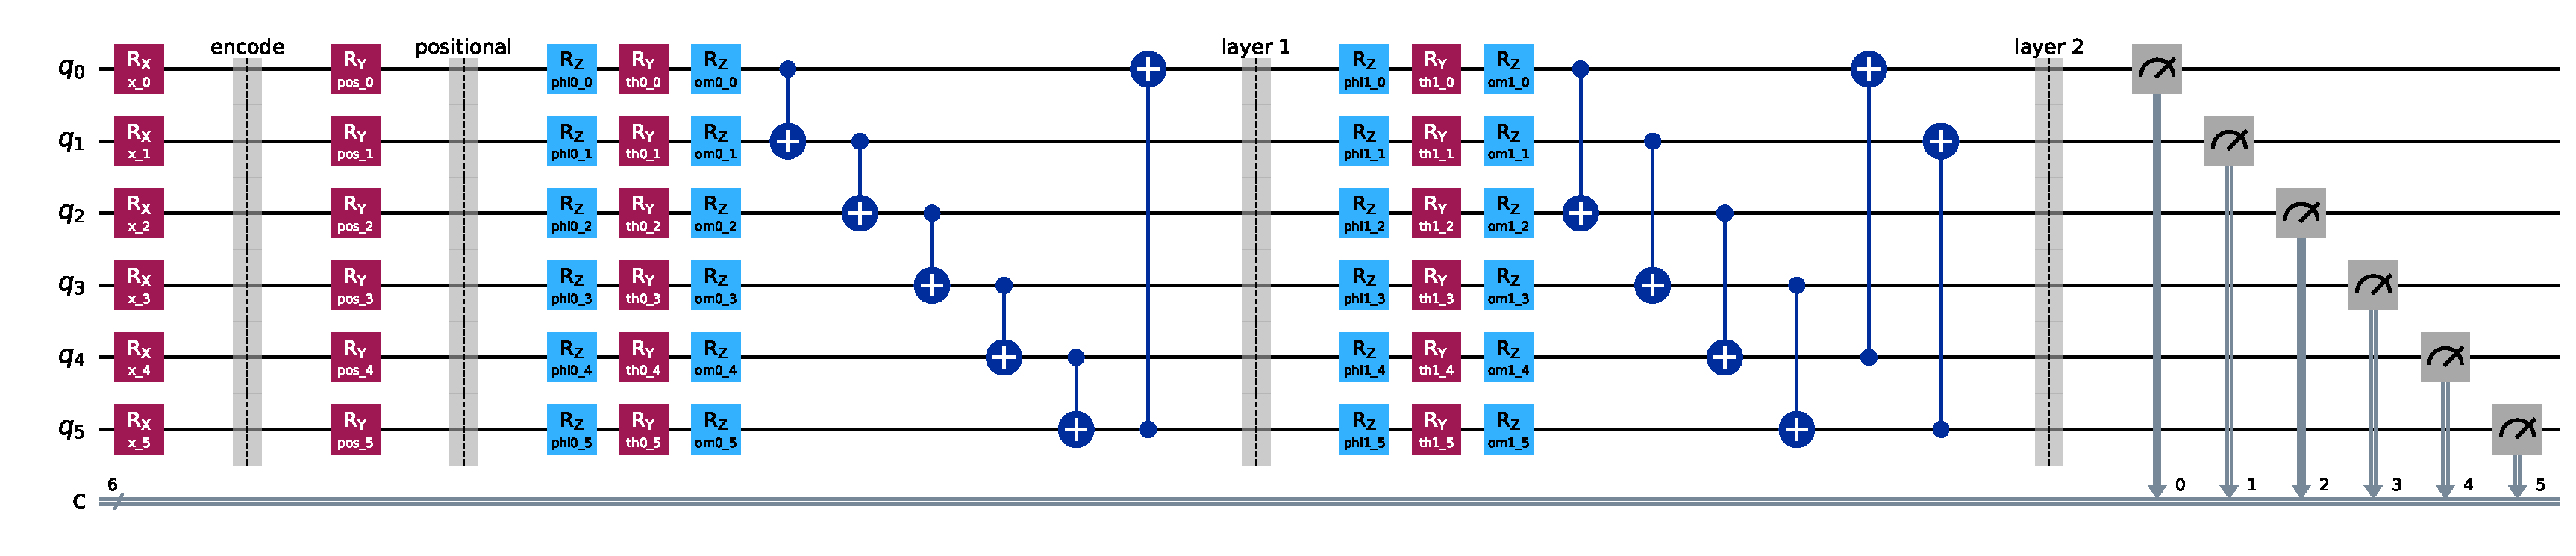
\includegraphics[width=0.99\textwidth]{figures/hvk1d_ansatz.pdf}\\[4pt]
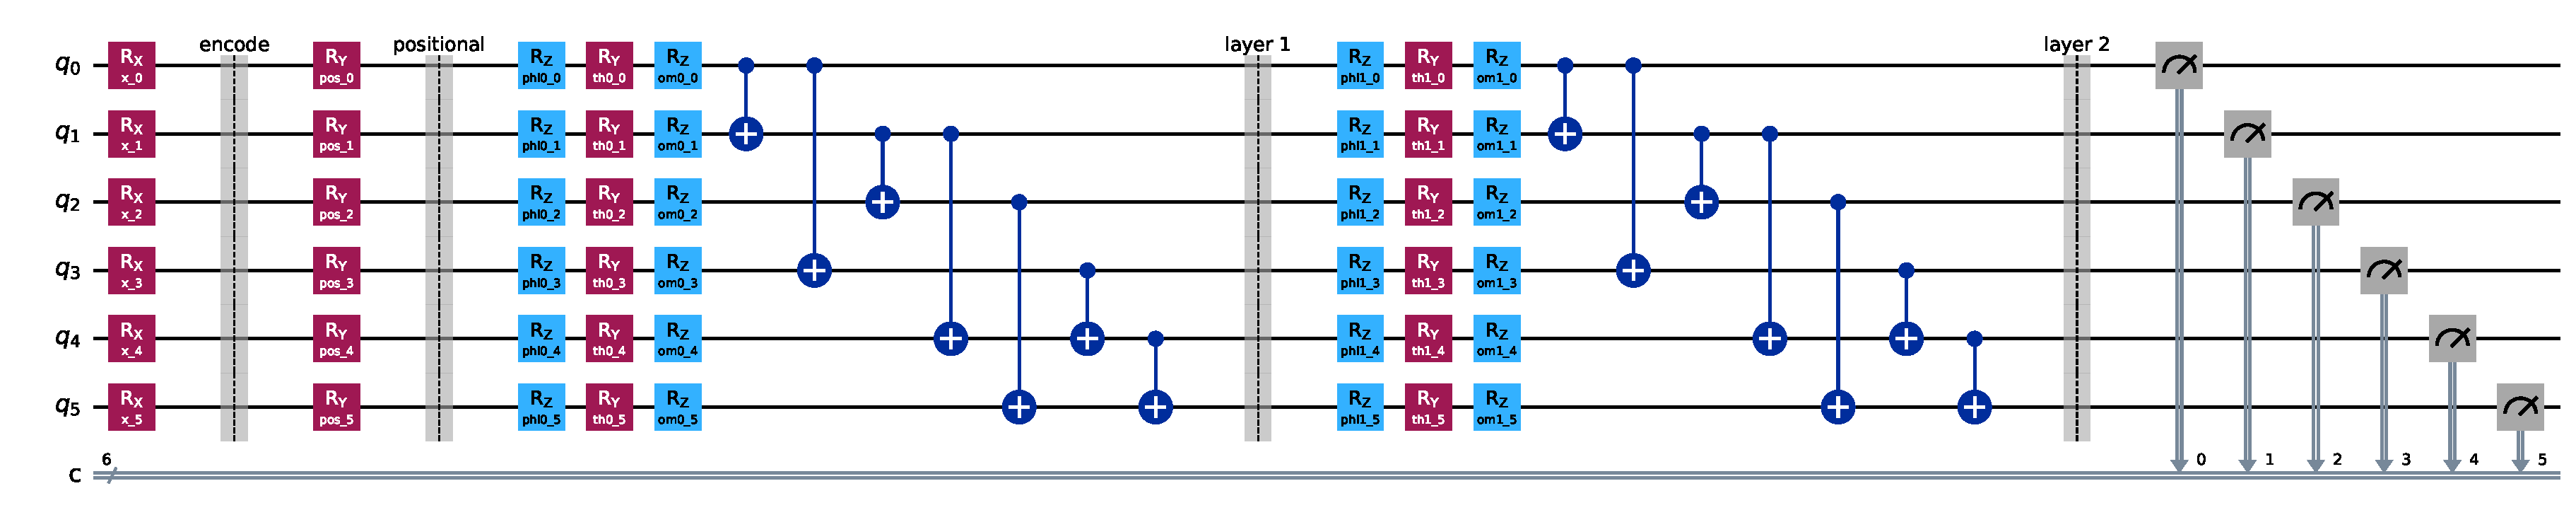
\includegraphics[width=0.99\textwidth]{figures/hvk2d_ansatz.pdf}
\caption{The HVK1D (top) and HVK2D (bottom) variational ansätze, exactly as executed (encoding $R_X$ rotations, positional $R_Y$ rotations, then two entangling layers of $R_Z$-$R_Y$-$R_Z$ single-qubit rotations with a CNOT ring for HVK1D or fixed grid-edge CNOTs for HVK2D). Both circuits were rebuilt gate-for-gate in Qiskit and validated against the original PennyLane training circuit before use in the hardware pilot of Section~\ref{sec:hardware_pilot}.}
\label{fig:hvk_ansatz}
\end{figure*}

Table~\ref{tab:variants} summarizes the tested variants. HVK1D uses a linear 6-qubit chain (5 nearest-neighbor bonds, 27-D observable vector); HVK2D arranges the same 6 qubits on a $2\times3$ lattice matching patch-boundary adjacency (19-D latent signature); a symmetric HVK1D variant adds a $\mathrm{U}(1)$-preserving coupling constraint; and a $D_4$-pooled HVK2D variant (Section~\ref{sec:symmetry}) group-averages the observable grid over the eight symmetries of the square, $\Phi_{D_4}(x)=\frac{1}{8}\sum_{g\in D_4}P_g^{-1}\Phi(gx)$, which is equivariant by construction. The IBM Cloud circuit probe reported in the supplement confirms both HVK1D and HVK2D compile to depth-18, 6-qubit circuits on a Heron-class basis.

\begin{table}[t]
\centering
\caption{HVK variants tested in this paper.}
\label{tab:variants}
\scriptsize
\resizebox{\columnwidth}{!}{%
\begin{tabular}{lccc}
\toprule
Variant & Topology & Latent dim. & Symmetry \\
\midrule
HVK1D & 6-qubit chain & 27-D & None (control) \\
HVK2D & $2\times3$ grid & 19-D & $D_4$-motivated only \\
Symmetric HVK1D & 6-qubit chain & 27-D & $\mathrm{U}(1)$ coupling \\
$D_4$-pooled HVK2D & $2\times3$ grid, pooled & 19-D & $D_4$-equivariant (proven) \\
\bottomrule
\end{tabular}%
}
\end{table}

\section{Experimental Setup}
\label{sec:protocol}
All image-reconstruction results in Sections~\ref{sec:sameset_results}--\ref{sec:hardware_pilot} use the single-image \textit{Monalisa} protocol developed for HVK: a fresh model is optimized directly on its target image, with no held-out split. They therefore measure per-image fitting and reconstruction capability, including hardware replay of those fitted checkpoints. The symmetry and restricted-entanglement diagnostics use the separate protocols stated in their respective sections; the exploratory training-dynamics material is addressed only as a provenance audit and is not retained as evidence. Held-out generalization and component necessity are evaluated under the resource-matched statistical protocol of the companion supplementary study (Section~\ref{sec:ablation_relationship}). All settings report MSE and PSNR $=20\log_{10}(1/\sqrt{\mathrm{MSE}})$; image settings additionally report SSIM. Full implementation settings and environment versions are given in the companion supplementary document.

\section{Results}
\label{sec:results}

\subsection{Reconstruction Across Six Real Image Datasets}
\label{sec:sameset_results}
For each image, we trained a fresh HVK2D model using nonoverlapping $8\times8$ patches (16 patches/image, 80--100 optimization steps). The sample covers CIFAR-10 \cite{Krizhevsky2009}, MNIST \cite{LeCun1998}, Fashion-MNIST \cite{Xiao2017}, and the PathMNIST, BloodMNIST, and PneumoniaMNIST subsets of MedMNIST v2 \cite{Yang2023}. Table~\ref{tab:sameset_multi_dataset} reports mean PSNR between $25.8$ and $41.6$~dB (SSIM $0.91$--$1.00$). This is a same-set fitting result across varied image structures, not a held-out generalization claim; the companion study provides the latter evaluation (Section~\ref{sec:ablation_relationship}).

\begin{table}[t]
\centering
\caption{HVK2D same-set reconstruction across six real image datasets (per-image trained, 80--100 steps, mean $\pm$ std over sampled images).}
\label{tab:sameset_multi_dataset}
\scriptsize
\resizebox{\columnwidth}{!}{%
\begin{tabular}{lccc}
\toprule
Dataset & $n$ images & PSNR (dB) & SSIM \\
\midrule
CIFAR-10 & 3 & $37.75\pm2.38$ & $0.9986\pm0.0003$ \\
MNIST & 3 & $25.77\pm2.23$ & $0.9783\pm0.0116$ \\
Fashion-MNIST & 3 & $34.55\pm3.05$ & $0.9980\pm0.0006$ \\
PathMNIST & 3 & $36.86\pm2.11$ & $0.9118\pm0.0627$ \\
BloodMNIST & 2 & $36.57\pm2.36$ & $0.9922\pm0.0063$ \\
PneumoniaMNIST & 2 & $41.60\pm0.98$ & $0.9985\pm0.0006$ \\
\bottomrule
\end{tabular}%
}
\end{table}

\subsection{Scope and Adaptation Across Images}
\label{sec:no_generalization}
A model optimized on one image alone does not transfer zero-shot to a structurally different image: on \textit{Monalisa}, zero-shot transfer to a second image reaches only $8.31$~dB PSNR ($\mathrm{SSIM}=0.1044$), while extending training to include the second image recovers $28.63$~dB ($\mathrm{SSIM}=0.9858$). This confirms that the per-image results above measure per-image optimization and reconstruction capability, not held-out generalization --- consistent with how we scope every claim in this paper, and precisely the distinction the companion supplementary study's held-out protocol is designed to test (Section~\ref{sec:ablation_relationship}).

\subsection{A Real Hardware Reconstruction Pilot}
\label{sec:hardware_pilot}
Every result above is a noiseless-simulator result, a limitation we flagged rather than left implicit. We report a first step past it: a small but complete image-reconstruction pilot executed on real IBM Quantum hardware (\texttt{ibm\_fez}, a 156-qubit Heron-class processor), beyond the compiled-circuit feasibility probe documented in the supplement. For five images --- the full 16-patch \textit{Monalisa} benchmark and four native-resolution CIFAR-10 images (\textit{cat}, \textit{ship}$\times2$, \textit{airplane}), each optimized directly on its own target image following the same per-image protocol as every result in this paper --- we took an already-trained HVK1D/HVK2D checkpoint's exact learned parameters, rebuilt its measurement circuits gate-for-gate in Qiskit, verified the translation against the original PennyLane simulator to within numerical noise ($\leq 7.9\times10^{-4}$ maximum absolute error per observable across every patch; full validation numbers in the companion supplementary document), and then executed the same circuits on real hardware with 256 shots per measurement basis, a fixed per-basis shot budget rather than an adaptive shadow-tomography-style estimation scheme \cite{Huang2020Shadows}. The hardware-measured observables were decoded by the same trained classical decoder, with no retraining and no simulator involved anywhere in the reconstruction path.

Reconstructions from real, noisy hardware measurements retain recognizable image structure. \textit{Monalisa} reaches $25.90$~dB PSNR from hardware measurements, against a $37.99$~dB noiseless-simulator replay of the identical circuit (Figure~\ref{fig:hardware_reconstruction_monalisa}); the four CIFAR-10 images average $29.56\pm2.03$~dB on hardware against $42.69\pm3.84$~dB in simulation (Figure~\ref{fig:hardware_reconstruction_cifar}, Table~\ref{tab:hardware_pilot_summary}). The observed gap is consistent with noise in these unmitigated device executions, although the five-image pilot does not isolate individual noise sources. Every hardware reconstruction remains above the random-latent control range ($11$--$15$~dB in the companion supplementary study). The pilot used 176 circuits; the contemporaneous account-meter reading increased by 16 quantum-processor seconds, with the provenance limitation documented in the supplement.

\begin{table}[t]
\centering
\caption{Real IBM hardware reconstruction pilot (backend \texttt{ibm\_fez}, 256 shots/basis, no retraining). PSNR compares hardware-decoded and simulator-decoded reconstructions against the same ground-truth image.}
\label{tab:hardware_pilot_summary}
\scriptsize
\resizebox{\columnwidth}{!}{%
\begin{tabular}{lccc}
\toprule
Image & Patches & Sim.\ PSNR (dB) & HW PSNR (dB) \\
\midrule
Monalisa (HVK1D) & 16 & 37.99 & 25.90 \\
CIFAR cat (HVK2D) & 16 & 44.85 & 31.52 \\
CIFAR ship, hydrofoil (HVK2D) & 16 & 36.56 & 26.44 \\
CIFAR ship, sea boat (HVK2D) & 16 & 42.57 & 31.20 \\
CIFAR airplane (HVK2D) & 16 & 46.79 & 29.10 \\
\midrule
CIFAR mean $\pm$ std (4 images) & -- & $42.69\pm3.84$ & $29.56\pm2.03$ \\
\bottomrule
\end{tabular}%
}
\end{table}

\begin{figure*}[t]
\centering
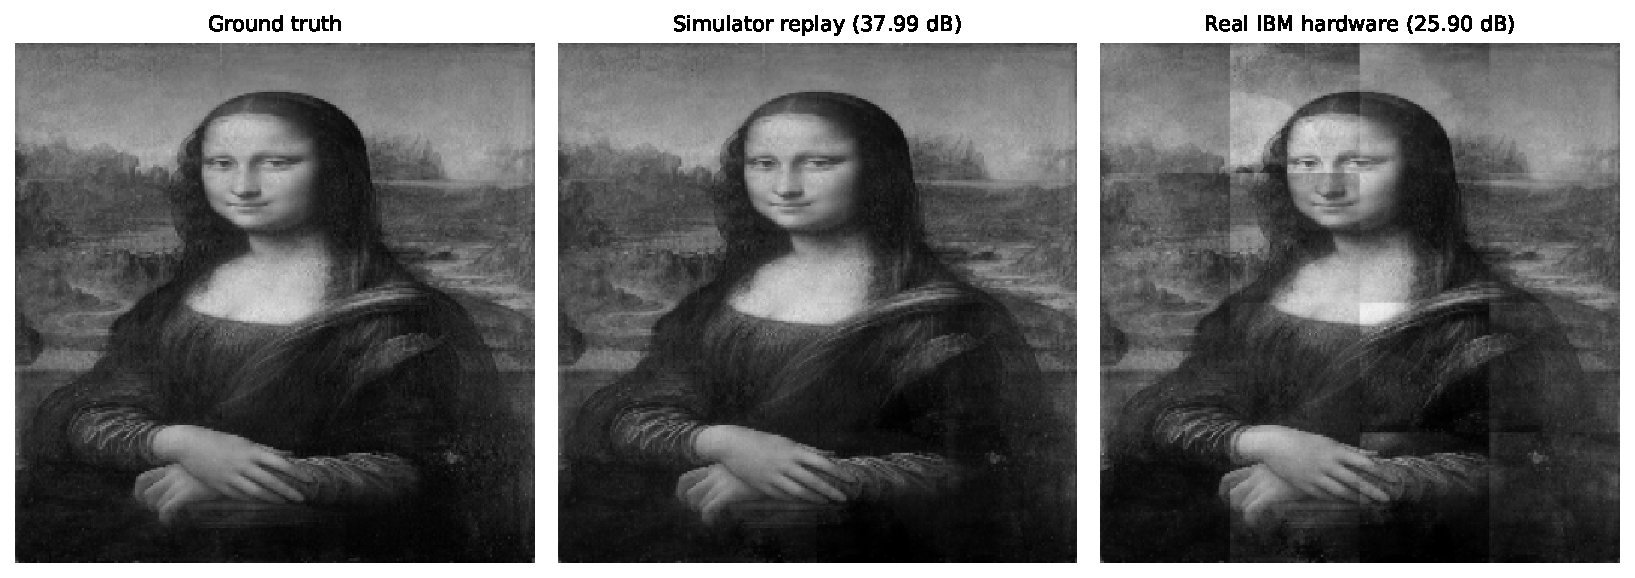
\includegraphics[width=0.96\textwidth]{figures/ibm_hardware_reconstruction_monalisa.pdf}
\caption{\textit{Monalisa} reconstructed from real IBM Quantum hardware measurements (right) against the same trained checkpoint's noiseless-simulator replay (center) and ground truth (left). The hardware image is visibly noisier and exhibits patch-boundary banding, while the subject remains recognizable.}
\label{fig:hardware_reconstruction_monalisa}
\end{figure*}

\begin{figure*}[t]
\centering
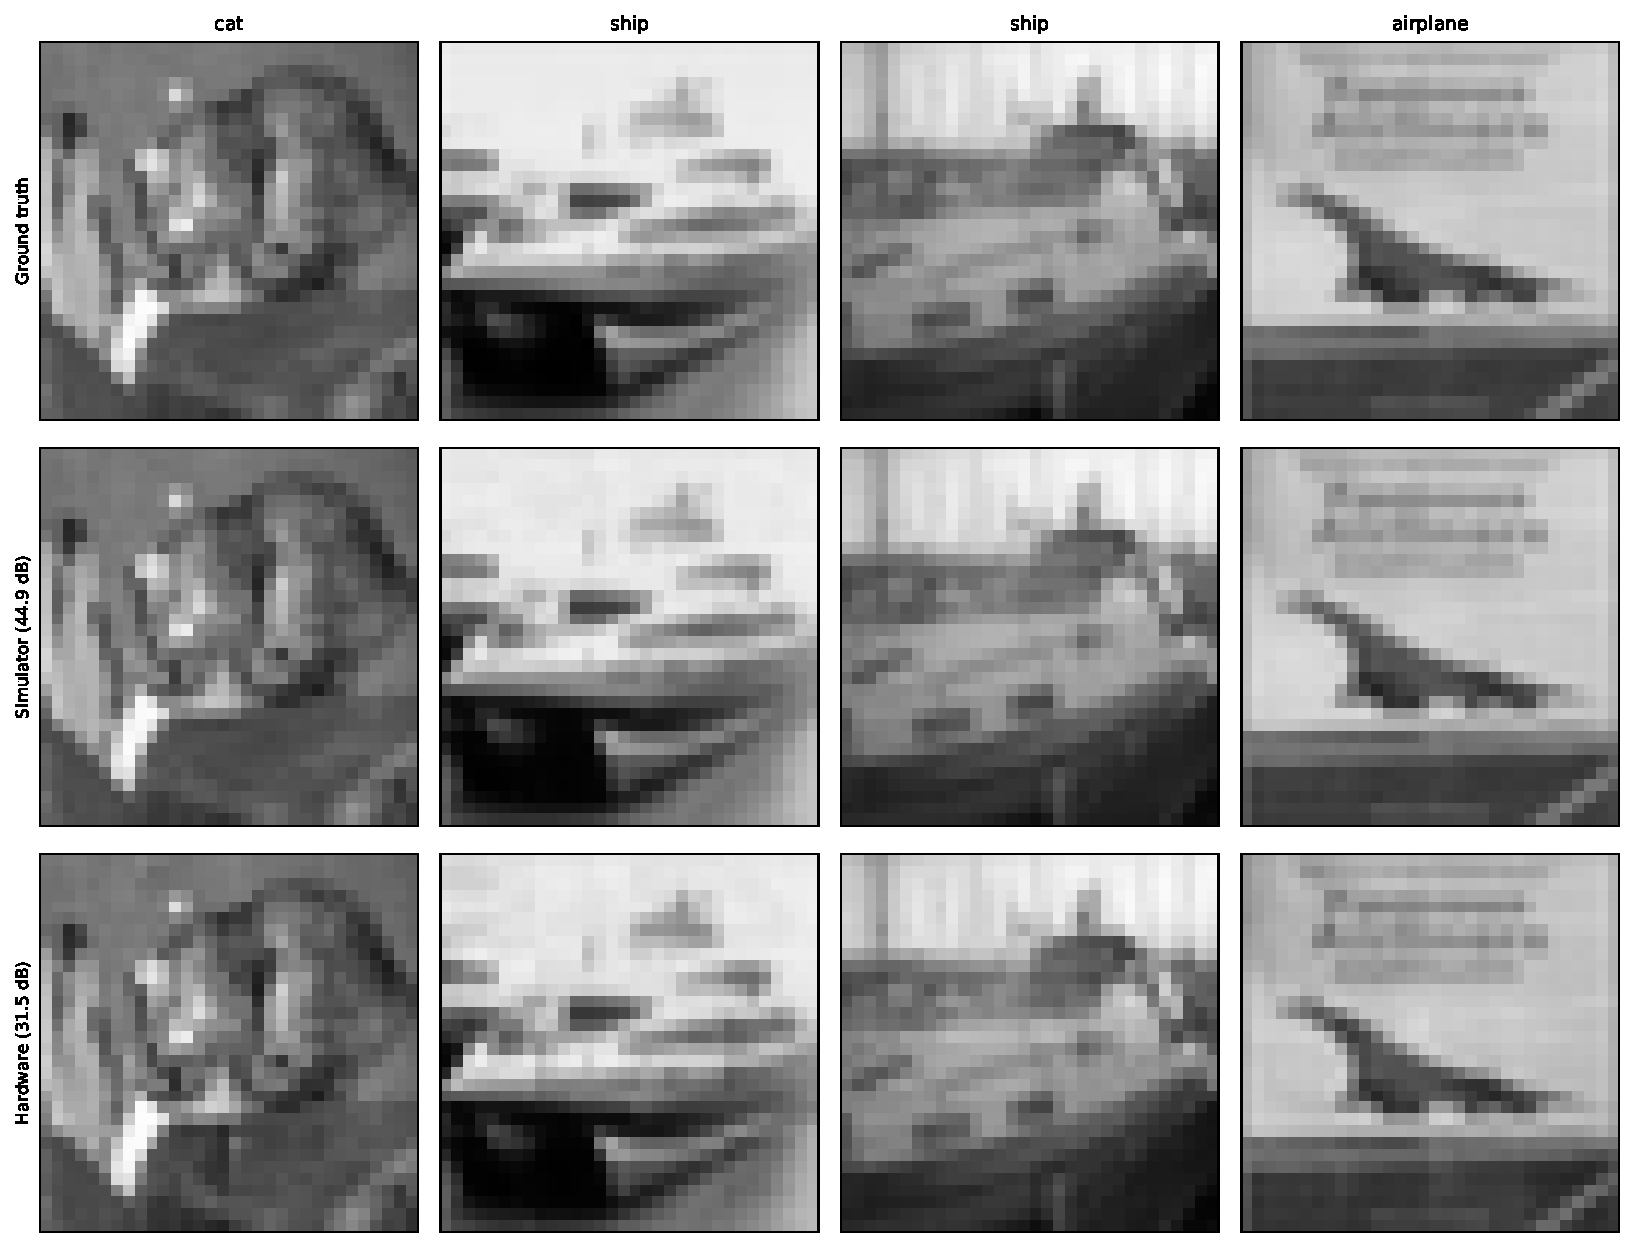
\includegraphics[width=0.96\textwidth]{figures/ibm_hardware_reconstruction_cifar.pdf}
\caption{Four CIFAR-10 images reconstructed from real IBM Quantum hardware measurements (bottom row) against noiseless-simulator replays of the same trained HVK2D checkpoints (middle row) and ground truth (top row).}
\label{fig:hardware_reconstruction_cifar}
\end{figure*}

Five images constitute a pilot, and we make no hardware-advantage claim. The narrower result is that the trained HVK observable channel remains visually and quantitatively informative in these device executions under the reported circuit and shot budget. Full methodology --- exact gate sequences, per-basis measurement construction, job IDs, and pre-submission local-validation results --- is documented in the companion supplementary document.

\subsection{Training-Dynamics Checkpoints Across System Sizes, Replayed on Real Hardware}
\label{sec:checkpoint_hardware_finite_size}
The finite-size comparison of Section~\ref{sec:finite_size_phase_transition} is a noiseless-simulator result. Using the same gate-for-gate checkpoint-replay methodology validated in Section~\ref{sec:hardware_pilot}, we extend it with a genuinely real-hardware complement: we trained fresh HVK1D checkpoints at $N\in\{4,6,8\}$ on two images (\textit{Monalisa}, CIFAR-10 \textit{cat}) for 200 real gradient-descent epochs, saved each checkpoint's exact learned parameters at eight epoch labels ($0,5,10,25,50,100,150,200$, matching the labels used elsewhere in this study), rebuilt each checkpoint's circuit for one representative patch, and executed all $48$ resulting circuits ($2$ images $\times$ $3$ system sizes $\times$ $8$ epoch labels) on \texttt{ibm\_fez} at $256$, $512$, and $1024$ shots. This is a single-patch, single-seed probe --- a lighter circuit budget than the full multi-patch reconstruction pilot above --- so it is a hardware-validation complement to Section~\ref{sec:finite_size_phase_transition}'s multi-seed simulator study, not a replacement for it: real device noise and single-patch/single-seed variance are both present in every point.

\begin{figure}[t]
\centering
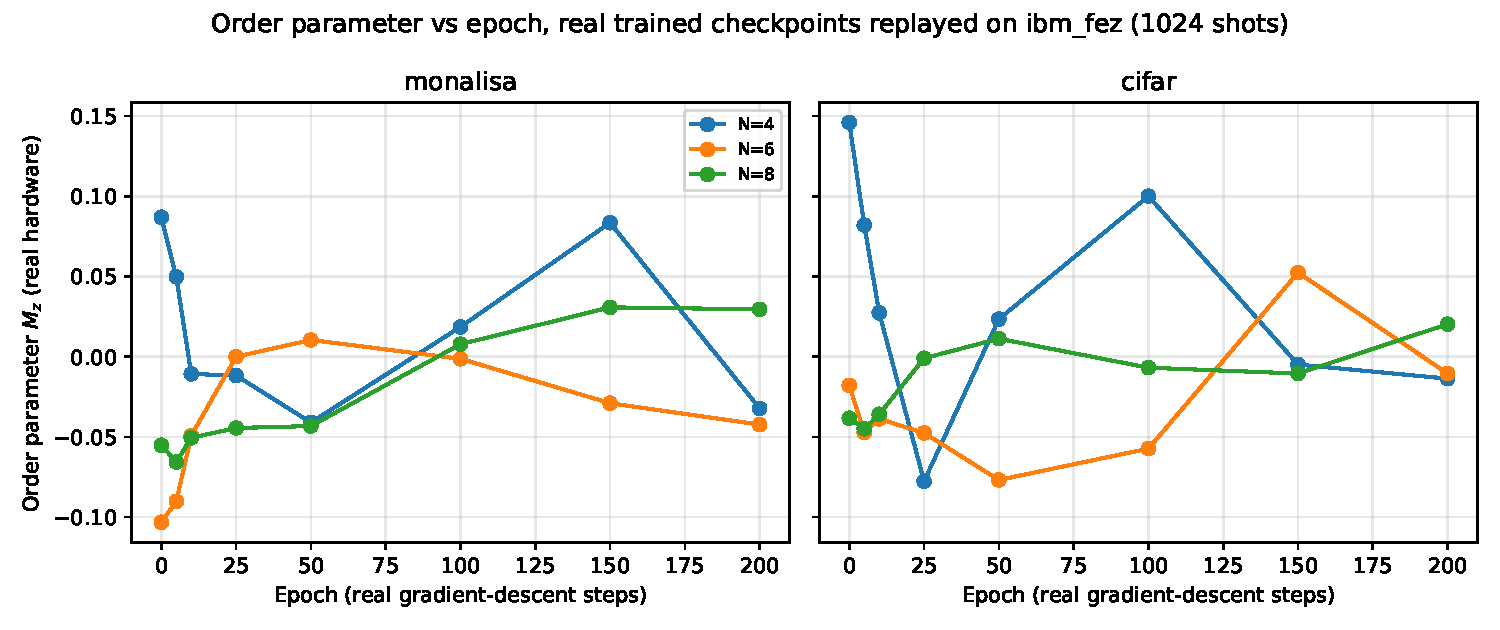
\includegraphics[width=\linewidth]{figures/checkpoint_hardware_order_parameter.pdf}
\caption{Order parameter $M_z(t)$ vs epoch from real trained HVK1D checkpoints ($N=4,6,8$), circuits rebuilt gate-for-gate and executed on real IBM Quantum hardware (\texttt{ibm\_fez}, 1024 shots), one representative patch per image.}
\label{fig:checkpoint_hardware_order_parameter}
\end{figure}

Figure~\ref{fig:checkpoint_hardware_order_parameter} shows the resulting curves are noisier and less structured than their noiseless-simulator counterparts in Figure~\ref{fig:finite_size_phase_transition}, as expected from single-shot-budget hardware measurement of a single patch rather than a change-magnitude trace averaged over multiple images and seeds. We do not apply the descriptive detection rule to these single-patch hardware traces; the figure establishes executable, non-degenerate hardware measurements across epochs, not independent confirmation of the detected change epochs in Table~\ref{tab:finite_size_phase_transition}. The same checkpoints were replayed on the IonQ simulator at the same three shot budgets (Section~\ref{sec:ionq_simulator}); full per-shot data are archived alongside this submission.

\subsection{Cross-Platform Replay on the IonQ Cloud Simulator}
\label{sec:ionq_simulator}
To test software-stack portability separately from device noise, we submitted the same checkpoint circuits through Qiskit to IonQ Quantum Cloud's ideal simulator (\texttt{ionq\_simulator}), with no hardware noise model enabled \cite{IonQBackends}. At each of 256, 512, and 1024 shots, one job contained 48 circuits spanning two images, $N\in\{4,6,8\}$, and eight epochs. All circuits completed, and the mean absolute $M_z$ deviation from the independently sampled 1024-shot trace decreased from $0.0257$ (256 shots) to $0.0213$ (512 shots). A separate 48-circuit, three-basis job reproduced the decreasing $R_{ES}(t)$ shape at 1024 shots.

\begin{figure}[t]
\centering
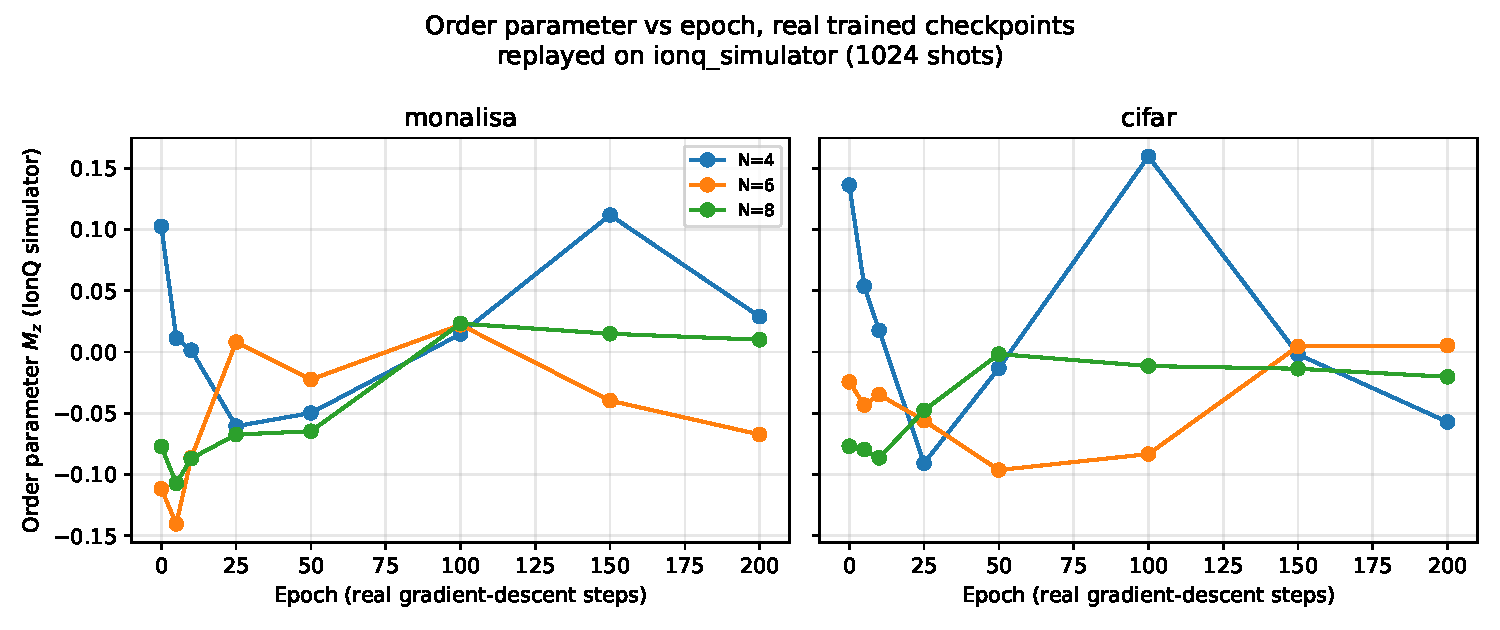
\includegraphics[width=\linewidth]{figures/checkpoint_ionq_order_parameter.pdf}
\caption{Order parameter $M_z(t)$ vs epoch from the same real trained HVK1D checkpoints as Figure~\ref{fig:checkpoint_hardware_order_parameter} ($N=4,6,8$), replayed on the IonQ ideal cloud simulator (\texttt{ionq\_simulator}, 1024 shots) instead of real IBM hardware.}
\label{fig:checkpoint_ionq_order_parameter}
\end{figure}

Figure~\ref{fig:checkpoint_ionq_order_parameter} shows this simulator trace directly, rather than only the summary deviation statistics above: a noiseless, shot-sampling-only analogue of Figure~\ref{fig:checkpoint_hardware_order_parameter}'s hardware traces, same checkpoints and circuits, no device noise. As above, we do not apply the descriptive detection rule of Eq.~\ref{eq:critical_epoch} to these single-patch traces. This is an ideal cloud-simulator portability check, not an IonQ-QPU result; job identifiers, estimator details, and per-circuit summaries are reported in the supplement. The corresponding IonQ $R_{ES}(t)$ replay is shown alongside its own hardware counterpart in Section~\ref{sec:checkpoint_hardware_energy_entanglement}.

\subsection{Noise/Shot Trade-off: A Free Simulator Complement}
\label{sec:hardware_robustness}
The five-image pilot above used a single shot budget (256/basis) and one execution per image, which bounds how much it can say about noise sensitivity on its own. Real IBM Quantum time is a scarce free-tier resource, so we separate what a \emph{calibrated device-noise simulation} can establish at zero hardware cost from what genuinely requires hardware. Using \texttt{qiskit-aer} with the live calibration snapshot of \texttt{ibm\_fez} (\texttt{FakeFez}, no quantum-processor time consumed), we replay the same already-trained checkpoints' circuits at four shot budgets (256/512/1024/4096 shots per basis, three repeated executions each) and compare against both the noiseless-simulator ceiling and the real-hardware point already reported above.

\begin{figure}[t]
\centering
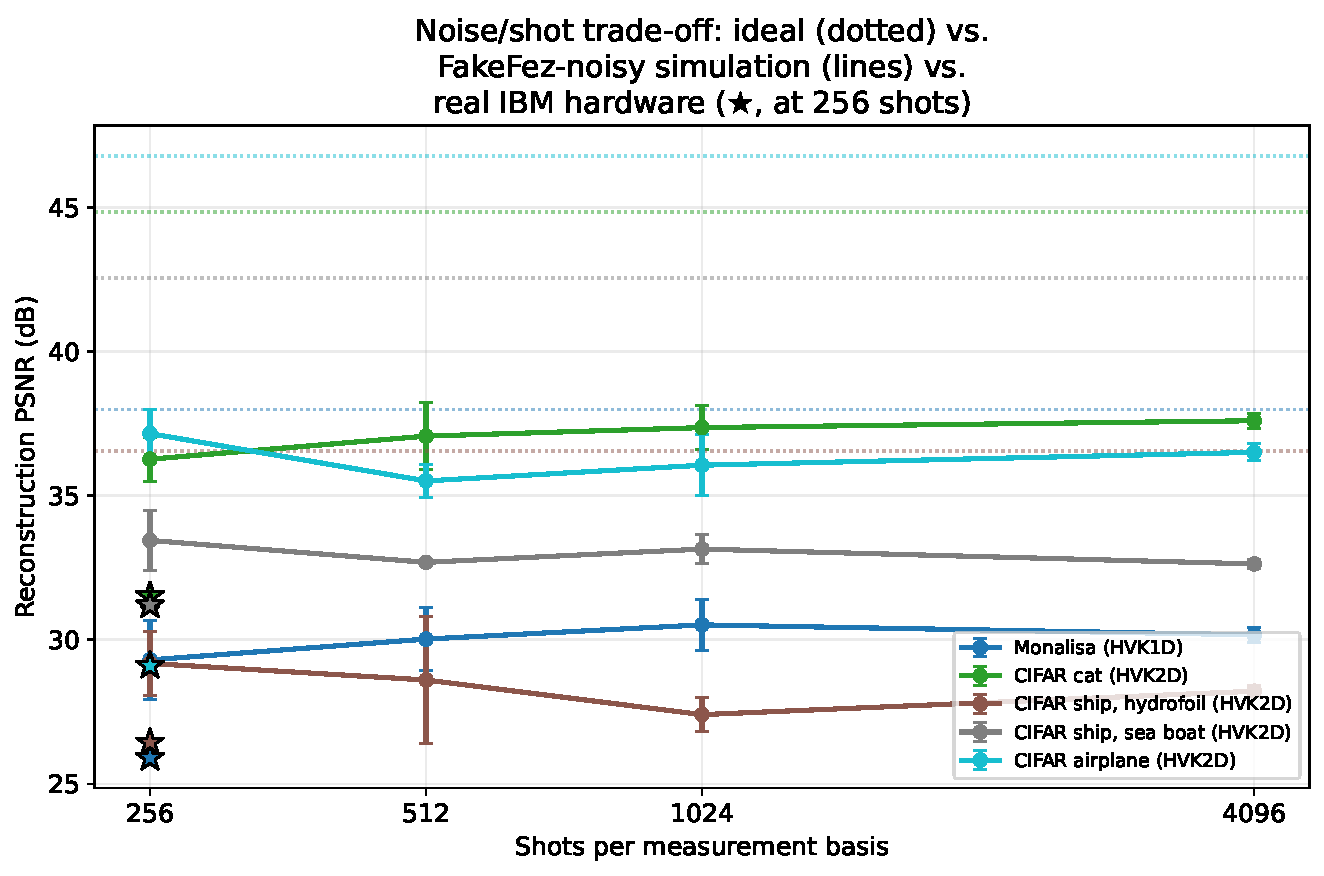
\includegraphics[width=\linewidth]{figures/hardware_robustness_shot_sweep.pdf}
\caption{Calibrated device-noise simulation (\texttt{FakeFez}, mean $\pm$ std over three executions). Dotted lines show noiseless ceilings and stars show real-hardware measurements. Increasing 256 to 4096 shots changes mean PSNR by only $-0.05$~dB.}
\label{fig:hardware_robustness_shot_sweep}
\end{figure}

Two findings follow, averaged over the five checkpoints. First, shot noise accounts for only part of the noiseless-to-real gap: moving from the noiseless ceiling to a calibrated-noise simulation at the same 256-shot budget already costs $8.68$~dB on average, before any real device is involved. Second, more shots does not reliably recover it: increasing to 4096 shots per basis changes PSNR by only $-0.05$~dB on average across the five checkpoints, with individual images ranging from a $1.33$~dB gain to a $0.96$~dB loss --- at this circuit size and shot range, shot count is not a lever that reliably improves reconstruction quality. Comparing the 256-shot noisy simulation directly against the real-hardware point isolates what the calibration snapshot does \emph{not} capture: a further $4.24$~dB average gap (range $2.25$--$8.06$~dB across images), attributable to device effects a single calibration snapshot does not fully capture --- drift between calibration and execution, crosstalk, and correlated errors chief among them. The airplane image is the clear outlier ($8.06$~dB residual gap, roughly double any other image), which we report rather than exclude; a single-execution, five-image pilot cannot distinguish an image-specific effect from ordinary job-to-job variation. This calibrated-noise simulation is a free, repeatable complement to the pilot, not a substitute for it: it bounds how much of the observed hardware gap is attributable to modeled device noise versus unmodeled effects, using zero additional quantum-processor time.

\subsection{Real-Hardware Anchor Points: Repeated Execution and a Second Backend}
\label{sec:hardware_anchors}
The simulated trade-off above is bounded, in turn, by whether it actually reflects real devices. We spent a small, explicitly quota-tracked slice of the free-tier IBM Quantum allowance (four jobs, well under $1\%$ of the monthly limit) confirming it directly: the same two checkpoints (\textit{Monalisa}, CIFAR \textit{cat}) replayed with no retraining on \texttt{ibm\_marrakesh} and \texttt{ibm\_kingston} --- two backends distinct from the original pilot's \texttt{ibm\_fez} --- at the original 256-shot budget and, separately, at 1024 shots.

\begin{table}[t]
\centering
\caption{Real-hardware anchor points: same checkpoints, no retraining, on two further backends. The original pilot's \texttt{ibm\_fez} point is shown for reference.}
\label{tab:hardware_anchors}
\scriptsize
\begin{tabular}{lccc}
\toprule
Image & Backend & Shots & PSNR (dB) \\
\midrule
Monalisa & ibm\_fez (original pilot) & 256 & 25.90 \\
Monalisa & ibm\_marrakesh & 256 & 25.94 \\
Monalisa & ibm\_kingston & 1024 & 26.10 \\
CIFAR cat & ibm\_fez (original pilot) & 256 & 31.52 \\
CIFAR cat & ibm\_kingston & 256 & 28.93 \\
CIFAR cat & ibm\_kingston & 1024 & 31.24 \\
\bottomrule
\end{tabular}
\end{table}

\textit{Monalisa} reproduces almost exactly across backends at matched shots ($25.94$ vs.\ $25.90$~dB, \texttt{ibm\_marrakesh} vs.\ \texttt{ibm\_fez}), and gains only $0.16$~dB from quadrupling shots to 1024 --- consistent with the simulated finding above that shot count is not a reliable lever. The CIFAR \textit{cat} point is the more informative one: on \texttt{ibm\_kingston} at the original 256-shot budget it reaches $28.93$~dB, $2.59$~dB below the \texttt{ibm\_fez} pilot point, while its own 1024-shot execution on the same backend recovers to $31.24$~dB, within $0.28$~dB of the original. This is real job-to-job and backend-to-backend variation of a magnitude comparable to the unmodeled residual identified by the simulator comparison (Section~\ref{sec:hardware_robustness}) --- direct evidence, not merely a simulated bound, that a single 256-shot execution on a single backend is not yet a stable estimate of this pipeline's hardware performance, and that repeated execution matters at least as much as backend choice or shot count individually.

\subsection{Provable \texorpdfstring{$D_4$}{D4} Symmetry}
\label{sec:d4}
\label{sec:symmetry}
A $D_4$-pooled HVK2D observable-grid map is equivariant to the eight symmetries of the square \emph{by construction}: $\Phi_{D_4}(x)=\frac{1}{8}\sum_{g\in D_4}P_g^{-1}\Phi(gx)$ averages the unpooled map over the group orbit, so $\Phi_{D_4}(hx)=P_h\Phi_{D_4}(x)$ for every $h\in D_4$ up to floating-point error. We verify this numerically over 7000 patch transforms of cached CIFAR images (Table~\ref{tab:d4_equivariance}, Figure~\ref{fig:d4_equivariance}): the pooled map's equivariance error is $9.57\times10^{-17}\pm1.26\times10^{-17}$ (floating-point noise), while the original unpooled positional map is not measurably more symmetric than a local/raw control ($0.815\pm0.129$ vs.\ $0.837\pm0.131$) --- confirming the unpooled map is only $D_4$-\emph{motivated} by the patch grid's geometry, not empirically equivariant, and that only the explicit pooling construction delivers the property. This is currently a feature-grid-level construction and numerical diagnostic rather than a component of the trainable reconstruction pipeline; integrating it end-to-end (Section~\ref{sec:limitations}) is concrete future work.

\begin{table}[t]
\centering
\caption{$D_4$ equivariance error for unpooled and pooled observable-grid maps (lower is better; pooled map is group-averaged over all eight square symmetries).}
\label{tab:d4_equivariance}
\scriptsize
\begin{tabular}{l@{\hspace{2em}}c@{\hspace{2em}}c}
\toprule
Model & Mean error & Std. error \\
\midrule
$D_4$-pooled HVK2D & $9.57\times10^{-17}$ & $1.26\times10^{-17}$ \\
No positional encoding & $7.40\times10^{-1}$ & $1.52\times10^{-1}$ \\
HVK2D positional & $8.15\times10^{-1}$ & $1.29\times10^{-1}$ \\
Local/raw & $8.37\times10^{-1}$ & $1.31\times10^{-1}$ \\
\bottomrule
\end{tabular}
\end{table}

\begin{figure}[t]
\centering
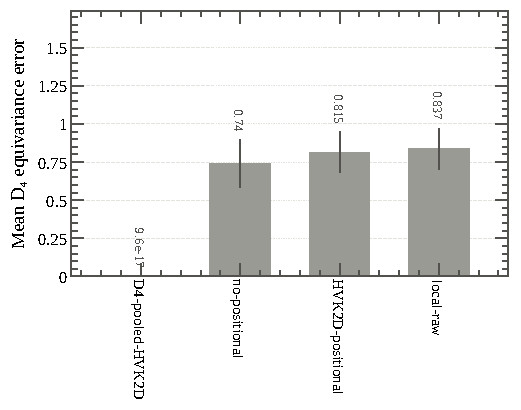
\includegraphics[width=\linewidth]{figures/d4_equivariance_summary.pdf}
\caption{$D_4$ equivariance diagnostic. The unpooled positional map is not equivariant; the group-pooled map is equivariant to numerical precision.}
\label{fig:d4_equivariance}
\end{figure}

\subsection{Entanglement Necessity in the Nonlocal-Structure Protocol}
\label{sec:entanglement_necessity}
This diagnostic is deliberately constructed to reward pair-observable structure: the target is a fixed synthetic function of \emph{simulated} patch features not concatenated into any candidate's own input block (the companion supplement gives the leakage-audit procedure that rules out circularity), and every control receives the same raw inputs as HVK2D. Table~\ref{tab:hvk_pair_diagnostic} and Figure~\ref{fig:hvk_pair_diagnostic} report the result across five seeds: HVK2D's entangling observable channel reaches mean $R^2=0.9735$ ($32.77$~dB PSNR), a $17.74$~dB improvement over a no-entanglement control ($R^2=0.019$) and $18.52$~dB over random-VQC latents ($R^2=-0.173$); freezing the quantum circuit (features fixed, only readout trained) still reaches $R^2=0.853$, while a parameter-matched classical control ($R^2=-0.030$) and a frozen-classical control ($R^2=-0.903$) fail outright. This is evidence that an entangling pair-observable channel is \emph{representationally necessary within the tested feature class and fixed linear-readout protocol} to fit this target.

\begin{table*}[t]
\centering
\caption{HVK2D restricted pair-correlation diagnostic across five seeds. Deliberately favorable to pair-observable structure; evidence for entanglement-necessity under a matched linear readout.}
\label{tab:hvk_pair_diagnostic}
\scriptsize
\begin{tabular}{lccc}
\toprule
Model & Mean MSE & Mean PSNR (dB) & Mean $R^2$ \\
\midrule
HVK2D entangling observables & $8.5969\times10^{-4}$ & 32.77 & 0.9735 \\
Freeze quantum & $4.7904\times10^{-3}$ & 27.34 & 0.8533 \\
No entanglement & $3.1461\times10^{-2}$ & 15.03 & 0.0191 \\
Raw-linear classical & $3.1654\times10^{-2}$ & 15.00 & 0.0133 \\
Parameter-matched classical & $3.3033\times10^{-2}$ & 14.82 & $-0.0297$ \\
Random VQC & $3.7616\times10^{-2}$ & 14.25 & $-0.1732$ \\
Freeze classical & $6.0973\times10^{-2}$ & 12.17 & $-0.9025$ \\
\bottomrule
\end{tabular}
\end{table*}

\begin{figure*}[t]
\centering
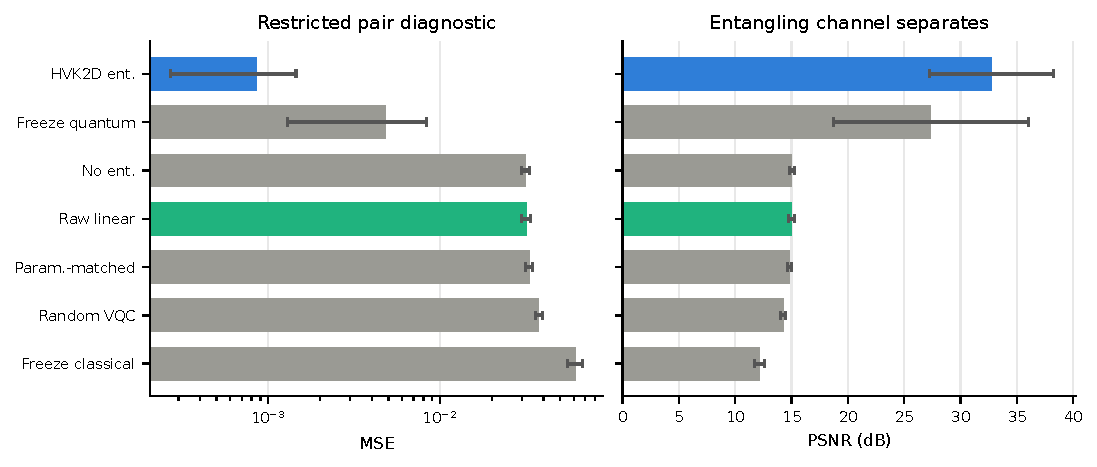
\includegraphics[width=0.96\textwidth]{figures/full_ablation_metric_comparison.pdf}
\caption{Restricted pair-correlation diagnostic summary (mean $\pm$ std over five seeds). The entangling observable feature map dominates every control on this deliberately favorable task.}
\label{fig:hvk_pair_diagnostic}
\end{figure*}

\subsection{Training-Dynamics Change-Point Diagnostic: A Corrected Multi-Seed Result}
\label{sec:phase_transition}
We test for abrupt changes in the learned representation during optimization. This is an exploratory change-point diagnostic on a magnetization-style summary, not a thermodynamic phase transition, a singularity, or an infinite-system claim. An earlier version was withdrawn after a provenance audit: the restricted-diagnostic trajectories previously shown were analytic interpolations produced for visualization rather than measurements from saved checkpoints, and the original multi-dataset traces were recorded during training, where HVK2D's training-mode forward pass deliberately adds Gaussian observable noise that confounds parameter evolution with injected jitter. The corrected runner evaluates a separate, noise-free forward pass in evaluation mode immediately after every optimizer update and tracks the resulting global order parameter $M_z(t)$, the mean of the $N$ local-$Z$ observables over all $P$ patches at optimizer step (epoch) $t$:
\begin{equation}
M_z(t) = \frac{1}{P N}\sum_{p=1}^{P}\sum_{i=1}^{N}\langle Z_i\rangle_p(t).
\label{eq:order_parameter}
\end{equation}
Detection uses the change magnitude $\mathcal{X}(t)=|M_z(t)-M_z(t-\Delta t)|$ (identically defined on $R_{ES}(t)$ in place of $M_z(t)$ for the energy-to-entanglement-ratio diagnostic of Section~\ref{sec:critical_temperature}), a per-run adaptive threshold $\theta$, and a detected change epoch $t_c$:
\begin{align}
\theta &= \operatorname{median}_t\big(\mathcal{X}(t)\big) + 2\operatorname{std}_t\big(\mathcal{X}(t)\big), \\
t_c &= \begin{cases}
\displaystyle\operatorname*{arg\,max}_t \mathcal{X}(t) & \text{if } \max_t \mathcal{X}(t) > \theta > 0, \\
\text{not detected} & \text{otherwise.}
\end{cases}
\label{eq:critical_epoch}
\end{align}
The threshold is computed per run from that run's own trace; it is not a fixed global constant or a null-calibrated statistical test. Thus ``detected'' means only that a run's sharpest observed change exceeds this descriptive within-run threshold. It does not supply a $p$-value, control a false-positive rate, or establish a physical transition.

Table~\ref{tab:phase_transition_corrected} reports the result across all six datasets (two images $\times$ two seeds each, 24 runs total). Detection is not universal: MNIST triggers in all four runs, BloodMNIST and PneumoniaMNIST in three of four, and CIFAR-10, Fashion-MNIST, and PathMNIST in two of four, for an overall descriptive rate of $16/24$ ($66.7\%$). Because the threshold is selected from the same trajectory it evaluates and the sample contains only two seeds per image, these rates are exploratory summaries rather than inferential evidence for dataset-specific transition probabilities.

\paragraph{A negative control: does the detector fire without a Hamiltonian?} The rate above says nothing about whether detection is actually driven by the learned Hamiltonian, so we ran the direct control this requires: the identical protocol applied to a \emph{classical-replacement} variant, in which the VQC is replaced by a fixed classical map and the Hamiltonian energy is identically zero throughout training, alongside matched Hamiltonian-on runs (\textit{Monalisa} and CIFAR-10 \textit{cat}, two seeds each, full 200-epoch budget). Table~\ref{tab:phase_transition_onoff} reports the result: all four Hamiltonian-on runs register a detection, but so do all four Hamiltonian-off runs. The detector does not distinguish a Hamiltonian-driven change from one this median-plus-two-standard-deviation threshold would find in a change-magnitude trace regardless of whether any physical energy term is present in the model at all. This sharpens, rather than merely repeats, the caveats already stated above: the $16/24$ rate should be read as a property of this specific descriptive threshold applied to this specific summary statistic, with no demonstrated dependence on the Hamiltonian term whose dynamics it is nominally tracking.

\begin{table}[t]
\centering
\caption{Corrected, noise-free training-dynamics diagnostic across all six datasets (2 images $\times$ 2 seeds/dataset).}
\label{tab:phase_transition_corrected}
\scriptsize
\begin{tabular}{lcccc}
\toprule
Dataset & $n$ & Detected & Mean $t_c$ & Mean $\mathcal{X}_{\max}$ \\
\midrule
CIFAR-10 & 4 & 2/4 & 64.0 & $0.0036\pm0.0009$ \\
MNIST & 4 & 4/4 & 98.75 & $0.0023\pm0.0012$ \\
Fashion-MNIST & 4 & 2/4 & 45.0 & $0.0027\pm0.0011$ \\
PathMNIST & 4 & 2/4 & 54.5 & $0.0038\pm0.0015$ \\
BloodMNIST & 4 & 3/4 & 96.0 & $0.0033\pm0.0012$ \\
PneumoniaMNIST & 4 & 3/4 & 103.0 & $0.0036\pm0.0008$ \\
\midrule
Total & 24 & $16/24$ & -- & -- \\
\bottomrule
\end{tabular}
\end{table}

\begin{table}[t]
\centering
\caption{Phase-transition detector, on/off control (200 epochs, two seeds/image). ``On'' is the standard Hamiltonian-regularized model; ``off'' is the classical-replacement variant with energy identically zero. The detector fires in every case tested, in both conditions.}
\label{tab:phase_transition_onoff}
\scriptsize
\begin{tabular}{llccc}
\toprule
Image & Seed & Hamiltonian & Detected & Critical epoch \\
\midrule
Monalisa & 0 & On & Yes & 4 \\
Monalisa & 0 & Off & Yes & 8 \\
Monalisa & 1 & On & Yes & 162 \\
Monalisa & 1 & Off & Yes & 23 \\
CIFAR cat & 0 & On & Yes & 97 \\
CIFAR cat & 0 & Off & Yes & 6 \\
CIFAR cat & 1 & On & Yes & 105 \\
CIFAR cat & 1 & Off & Yes & 1 \\
\midrule
Total & \multicolumn{2}{c}{On} & 4/4 & -- \\
Total & \multicolumn{2}{c}{Off} & 4/4 & -- \\
\bottomrule
\end{tabular}
\end{table}

\subsection{System-Size Sensitivity of the Detected Change Epoch}
\label{sec:finite_size_phase_transition}
Every result above is measured at a single, fixed system size (HVK2D's six-qubit grid). We therefore ask whether the descriptive change epoch depends on circuit width. HVK2D's grid topology is fixed at six qubits by construction, so this comparison uses HVK1D's parameterized chain topology. We reran the corrected protocol from Section~\ref{sec:phase_transition} at $N=4$, $N=6$, and $N=8$ qubits on two datasets (CIFAR-10 and MNIST), one image and two seeds each (four runs per size, 200 epochs). Three sizes and four runs per size are insufficient for finite-size scaling or critical-exponent analysis; the experiment is a sensitivity check on the diagnostic only.

All twelve runs register a detection under the same threshold rule (Table~\ref{tab:finite_size_phase_transition}), but the detected epoch is not monotonic in $N$: $10.0\pm12.7$ at $N=4$, $85.0\pm50.1$ at $N=6$, and $61.0\pm65.2$ at $N=8$. Three of the four $N=8$ traces stay near $M_z\approx0$ and trigger on small early changes, whereas one MNIST run develops a late excursion at $t_c=172$ that dominates the variance. The result therefore shows instability of this heuristic across width and initialization, not a scaling law or evidence of a critical point.

\begin{table}[t]
\centering
\caption{Finite-size comparison of the order-parameter diagnostic, HVK1D, CIFAR-10 + MNIST (1 image $\times$ 2 seeds per dataset per $N$).}
\label{tab:finite_size_phase_transition}
\scriptsize
\begin{tabular}{lcccc}
\toprule
$N$ (qubits) & $n$ & Detected & Mean $t_c$ & Std $t_c$ \\
\midrule
4 & 4 & 4/4 & 10.0 & 12.7 \\
6 & 4 & 4/4 & 85.0 & 50.1 \\
8 & 4 & 4/4 & 61.0 & 65.2 \\
\bottomrule
\end{tabular}
\end{table}

\begin{figure}[t]
\centering
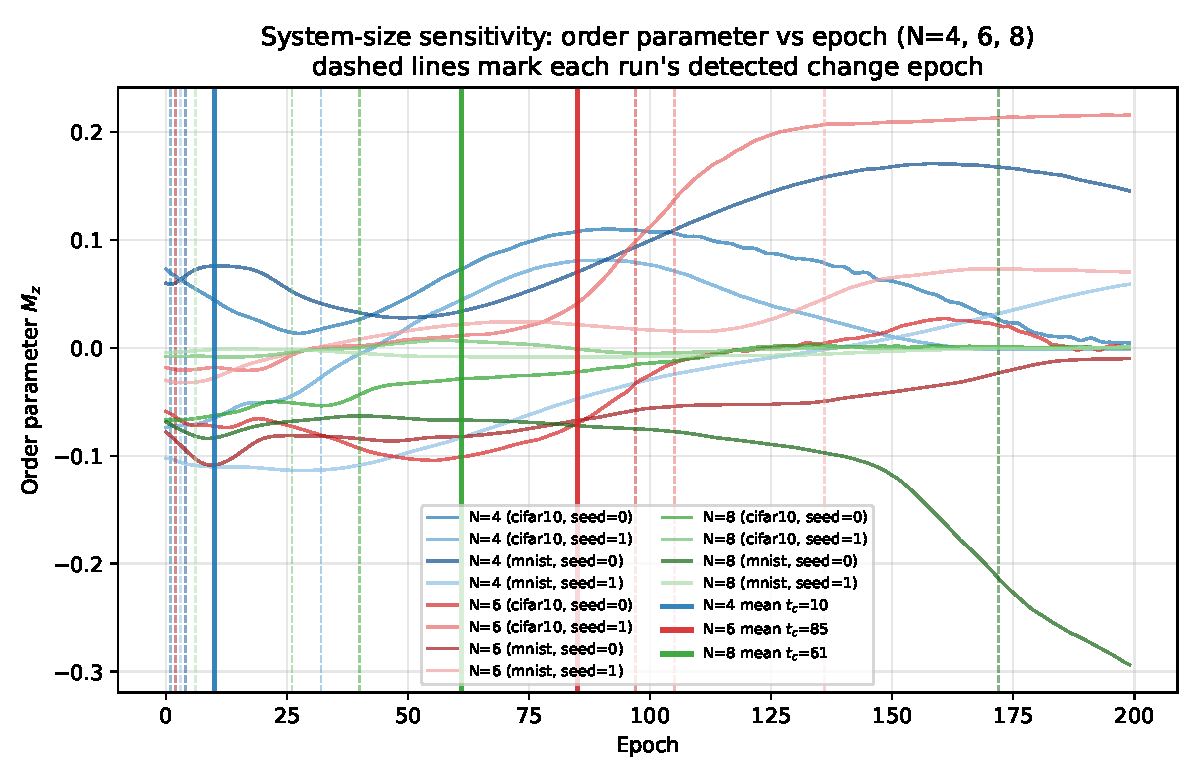
\includegraphics[width=\linewidth]{figures/finite_size_phase_transition.pdf}
\caption{Order parameter $M_z(t)$ vs epoch, HVK1D, $N=4$ (blue), $N=6$ (red), and $N=8$ (green), four runs each. Dashed lines mark within-run detected change epochs; solid lines mark per-$N$ means. Most $N=8$ traces stay near zero, while one late outlier drives much of the variance.}
\label{fig:finite_size_phase_transition}
\end{figure}

Table~\ref{tab:finite_size_phase_transition} summarizes per-run detections: each run's own change magnitude is thresholded independently, then the resulting change epochs are averaged, giving a non-monotonic mean ($10.0\to85.0\to61.0$). A complementary view averages the change-magnitude \emph{traces themselves} across the four runs at each $N$ before locating a peak, rather than averaging four independently-detected peak locations. This ensemble-mean view (Figure~\ref{fig:finite_size_mean_susceptibility}) shows the peak of $\langle|\Delta M_z(t)|\rangle$ shifting later with $N$: epoch $3$ at $N=4$, epoch $96$ at $N=6$, epoch $163$ at $N=8$ --- monotonic, in contrast to Table~\ref{tab:finite_size_phase_transition}. We report both because they are not the same statistic and can disagree: per-run thresholding is sensitive to whichever single epoch happens to cross that run's own noisy threshold, while the ensemble mean suppresses run-to-run idiosyncrasy at the cost of blurring together events that do not align in time across runs. The $N=4$ peak at epoch $3$ sits at the very start of training, where curves are dominated by initialization transients rather than a mid-training reorganization, and should be read with that caveat; $N=6$ produces the sharpest, best-separated peak of the three (Figure~\ref{fig:finite_size_mean_susceptibility}), while $N=8$'s peak is broad and comparable in height to its own baseline fluctuation. With four runs per $N$, the shaded $\pm$one-std bands in Figure~\ref{fig:finite_size_mean_susceptibility} are wide enough that we treat the monotonic peak-shift as a second exploratory observation alongside Table~\ref{tab:finite_size_phase_transition}'s non-monotonic one, not as a resolution of it.

\begin{figure}[t]
\centering
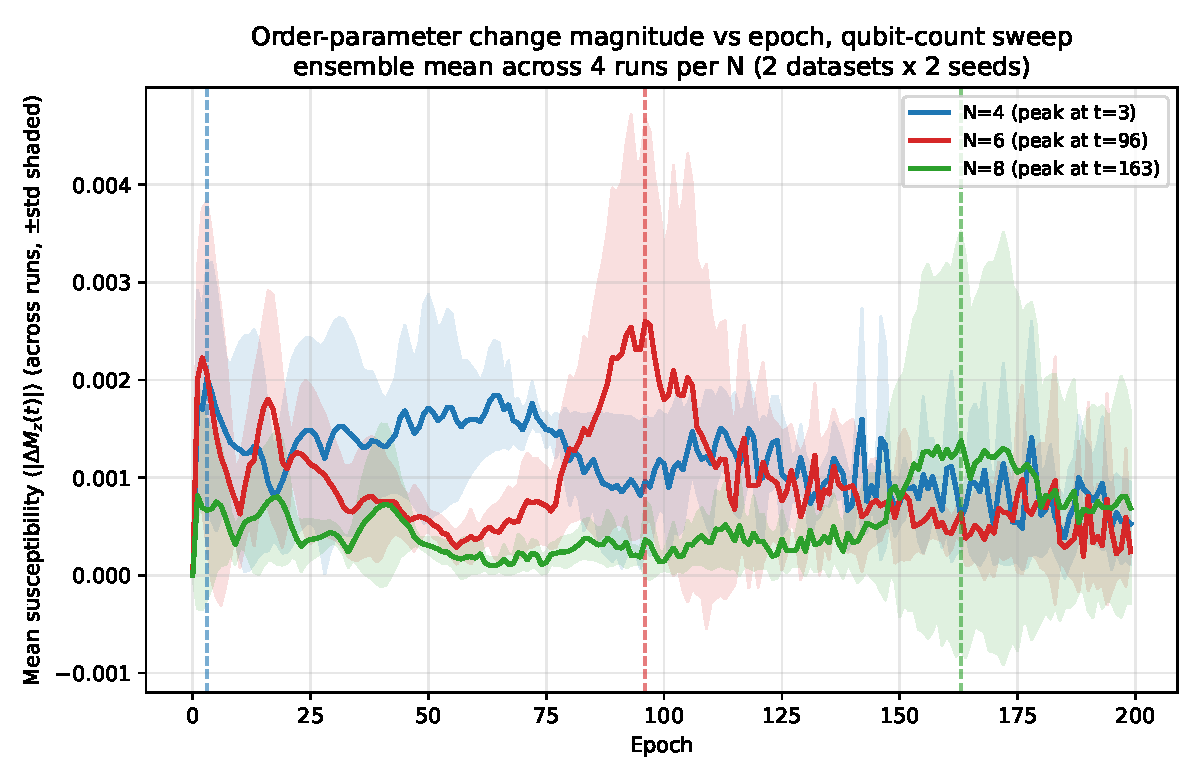
\includegraphics[width=\linewidth]{figures/finite_size_mean_susceptibility.pdf}
\caption{Ensemble-mean change magnitude $\langle|\Delta M_z(t)|\rangle$ vs epoch, averaged across the four runs at each $N$ before peak-finding (shaded: $\pm$one std across runs), $N=4$ (blue), $N=6$ (red), $N=8$ (green). Dashed vertical lines mark each curve's peak epoch. The peak shifts monotonically later with $N$ (epochs $3$, $96$, $163$), a different statistic from the per-run-averaged epochs in Table~\ref{tab:finite_size_phase_transition}.}
\label{fig:finite_size_mean_susceptibility}
\end{figure}

\subsection{A Second, Orthogonal Size Axis: MPS Bond Dimension}
\label{sec:bond_dimension_phase_transition}
Qubit count $N$ is a quantum circuit-width parameter; a second, purely classical size parameter enters before the circuit. We test whether the detected change epoch depends on MPS compression fidelity, holding $N=6$ fixed and varying $\chi$ on CIFAR-10. An initial two-seed, single-image ($\textit{cat}$) pass at $\chi\in\{1,2,4,8\}$ suggested richer compression might reduce initialization sensitivity ($\chi=4,8$ appeared to agree tightly); we extended $\chi\in\{4,6,8\}$ to five images (two seeds each, ten runs per $\chi$) to test whether that held up with more data. $\chi=1,2$ remain at their original one-image, two-seed scope.

All 34 runs trigger. The extended data both sharpens and revises the original two-seed reading. It sharpens the qualitative claim: at $n=10$, $\chi=4$, $\chi=6$, and $\chi=8$ now show visually near-identical ensemble-mean trajectories and overlapping $\pm$one-std bands throughout training (Figure~\ref{fig:bond_dimension_phase_transition}, Table~\ref{tab:bond_dimension_phase_transition}), while $\chi=1$ and $\chi=2$ remain clearly distinct from each other and from the $\chi\geq4$ group. It revises the quantitative claim: the original $\chi=4$/$\chi=8$ standard deviations ($4.0$/$2.0$ epochs) reflected only two seeds on one image and were misleadingly tight; at five images the true spread is far larger ($\mathrm{std}\approx60$ epochs for each of $\chi=4,6,8$), comparable to $\chi=1,2$'s spread rather than smaller than it. Read together, richer compression does not reduce run-to-run variance in this diagnostic --- the apparent tight agreement at $\chi=4,8$ was a small-sample artifact --- but it does produce indistinguishable \emph{mean} dynamics across $\chi\geq4$, a genuinely different and better-supported finding than the original two-seed pass suggested.

This is a different measurement from, but worth reading alongside, the companion supplementary study's single-seed finding that MPS bond dimension is non-monotonic for \emph{final reconstruction quality}: under a fixed step budget, $\chi=1$ and $\chi=2$ outperform the default $\chi=4$ on PSNR, with $\chi=8$ only partially recovering. The two results together suggest bond dimension has separable effects on \emph{where} training ends up (reconstruction quality, non-monotonic) versus \emph{the shape of the training-dynamics trace} (converges once $\chi\geq4$) --- a connection neither single result establishes on its own.

\begin{table}[t]
\centering
\caption{MPS bond-dimension comparison of the order-parameter diagnostic, HVK1D, $N=6$ fixed. $\chi=1,2$: CIFAR-10 \textit{cat}, 2 seeds. $\chi=4,6,8$: 5 CIFAR-10 images, 2 seeds each (10 runs).}
\label{tab:bond_dimension_phase_transition}
\scriptsize
\begin{tabular}{lcccc}
\toprule
$\chi$ (MPS bond dim.) & $n$ & Detected & Mean $t_c$ & Std $t_c$ \\
\midrule
1 & 2 & 2/2 & 88.5 & 86.5 \\
2 & 2 & 2/2 & 52.0 & 50.0 \\
4 & 10 & 10/10 & 73.8 & 60.9 \\
6 & 10 & 10/10 & 73.3 & 61.4 \\
8 & 10 & 10/10 & 72.5 & 60.1 \\
\bottomrule
\end{tabular}
\end{table}

\begin{figure}[t]
\centering
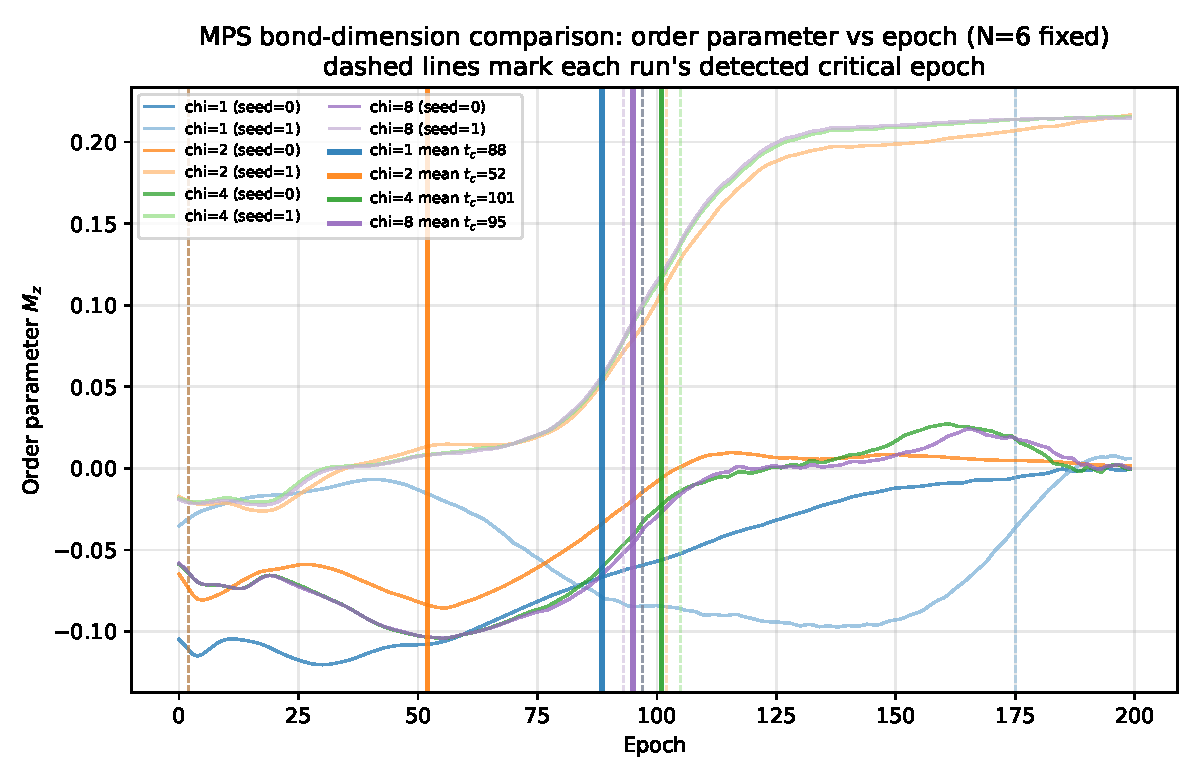
\includegraphics[width=\linewidth]{figures/bond_dimension_phase_transition.pdf}
\caption{Ensemble-mean order parameter $M_z(t)$ vs epoch ($\pm$one std, shaded), HVK1D, $N=6$ fixed. $\chi=1,2$: 1 image $\times$ 2 seeds. $\chi=4,6,8$: 5 images $\times$ 2 seeds (10 runs each). The $\chi\geq4$ curves are visually near-identical throughout training, while $\chi=1,2$ remain distinct from each other and from the $\chi\geq4$ group.}
\label{fig:bond_dimension_phase_transition}
\end{figure}

As an execution check, we also replayed trained checkpoints across the original four bond dimensions ($\chi\in\{1,2,4,8\}$, predating the $\chi=6$ / five-image simulator extension above) on real \texttt{ibm\_marrakesh} hardware and the IonQ ideal simulator at 256, 512, and 1024 shots. All checkpoint circuits completed and produced non-degenerate order parameters, but the single-patch, single-seed replay cannot confirm the cross-seed pattern above. The companion supplement reports the complete twelve-job audit trail, the hardware curves, and a three-basis $R_{ES}$ replay; it also documents why $\chi=1$ is excluded from the ratio because its product-state entropy reaches the numerical floor.

\subsection{Energy-to-Entanglement Ratio as an Orthogonal Diagnostic}
\label{sec:critical_temperature}
The learned Heisenberg energy provides a second scalar view of training. We define the signed energy-to-entanglement ratio
\begin{align}
R_{ES}(t)&=\frac{H(t)}{S},\\
H(t)&=\sum_i\Bigl[J_x^{(i)}\langle X_iX_{i+1}\rangle
J_y^{(i)}\langle Y_iY_{i+1}\rangle \nonumber\\
&\hspace{3.0em}+J_z^{(i)}\langle Z_iZ_{i+1}\rangle\Bigr].
\end{align}
where $S=\sum_i S_i$ is the fixed sum of von Neumann bond entropies from the classical MPS decomposition. This ratio has units of energy per entropy unit and is \emph{not} a thermodynamic temperature: no Gibbs state is fitted, no derivative $\partial S/\partial E$ is evaluated, and its negative sign reflects the learned signed Hamiltonian. The bond correspondence is clean only for HVK1D at six sites, so we track $R_{ES}(t)$ there on two CIFAR-10 images over four seeds and apply the same descriptive change-threshold rule to $|\Delta R_{ES}(t)|$.

\begin{figure}[t]
\centering
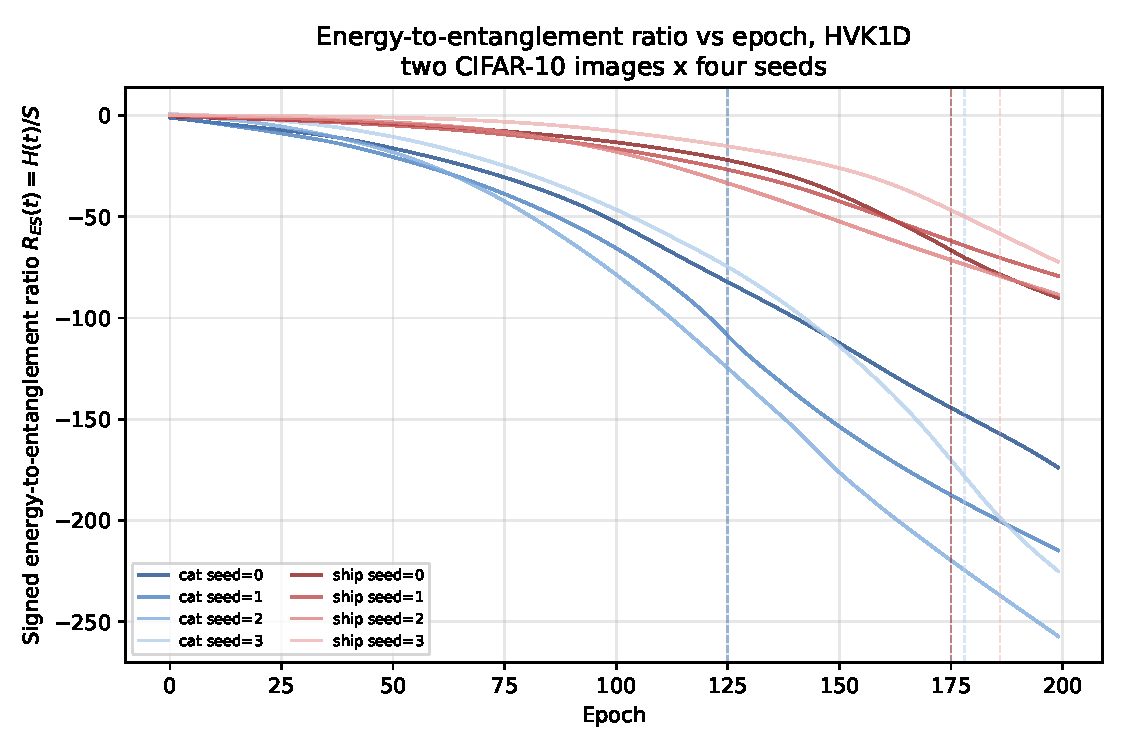
\includegraphics[width=\linewidth]{figures/critical_temperature_traces.pdf}
\caption{Signed energy-to-entanglement ratio $R_{ES}(t)=H(t)/S$ across training, HVK1D, two CIFAR-10 images $\times$ four seeds. The increasingly negative traces reflect the learned signed energy at fixed $S$; they are not temperature or cooling curves.}
\label{fig:critical_temperature}
\end{figure}

\begin{figure}[t]
\centering
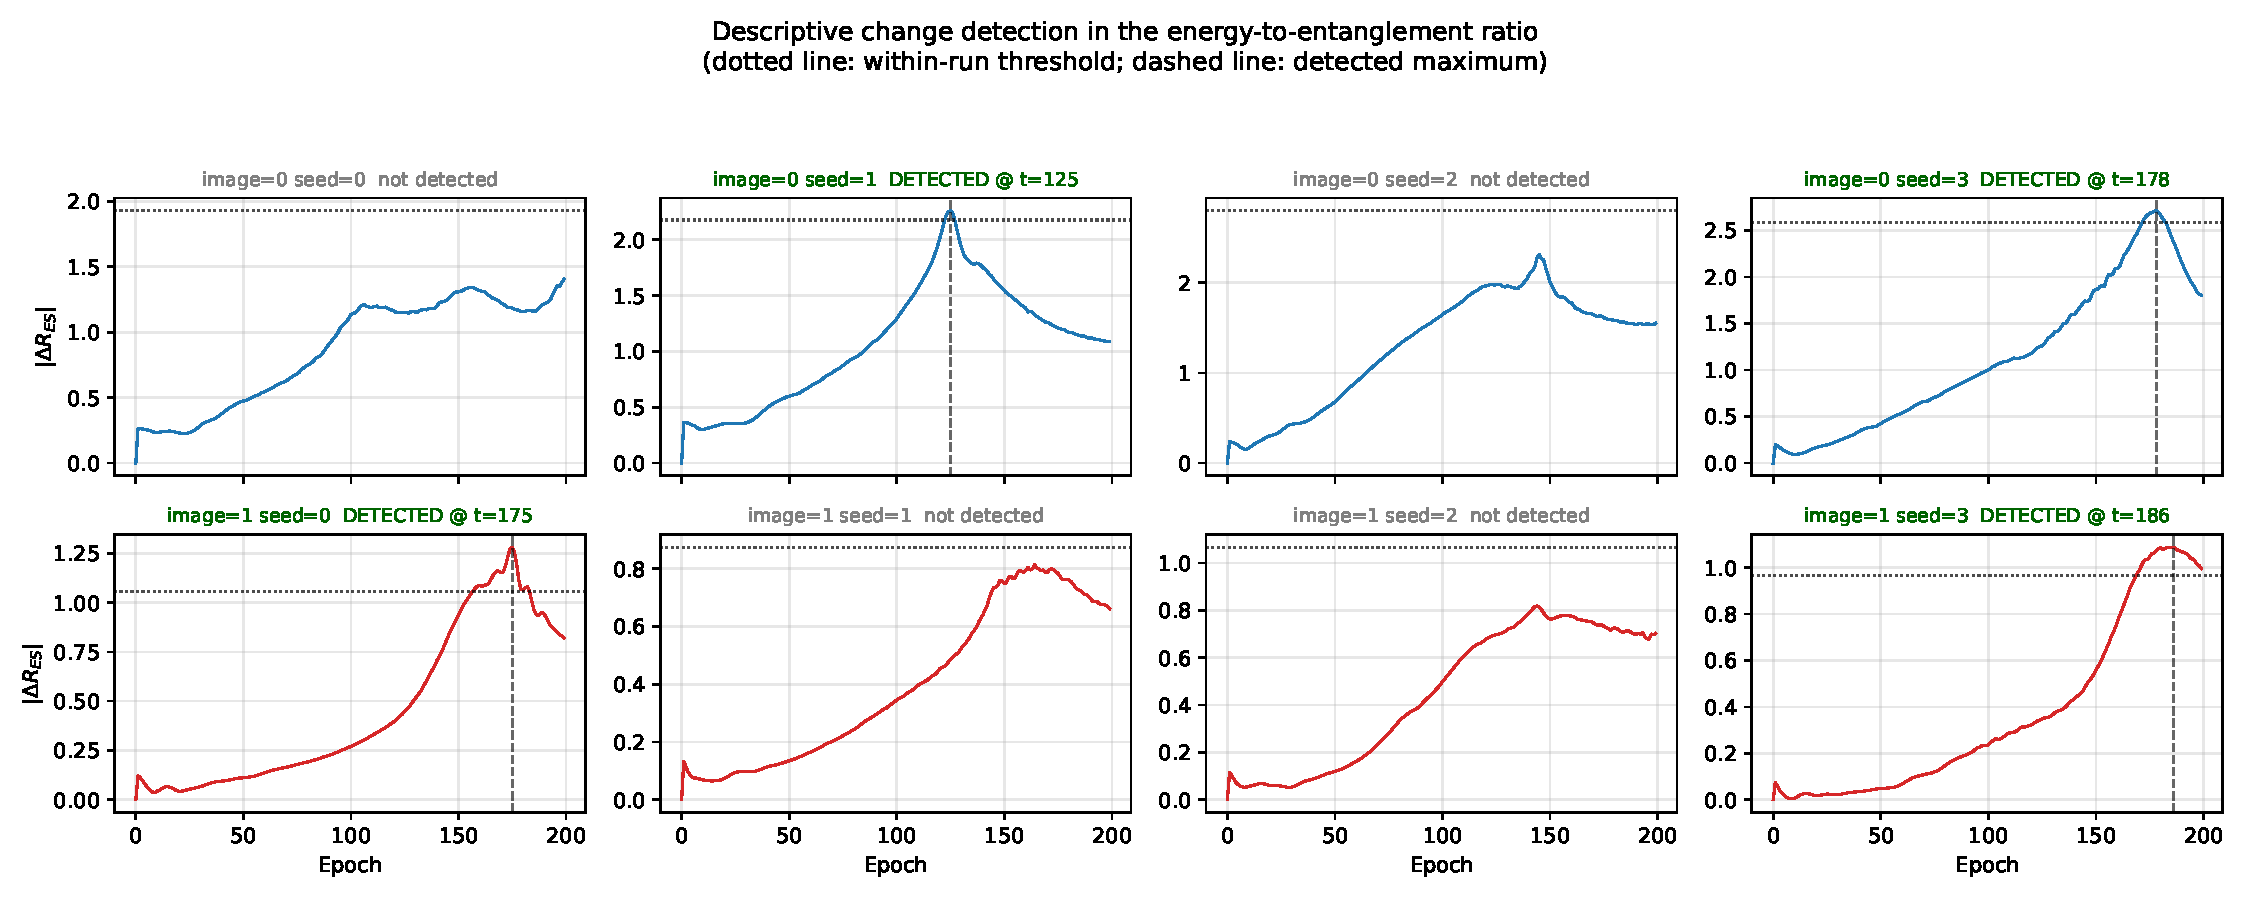
\includegraphics[width=\linewidth]{figures/critical_temperature_susceptibility.pdf}
\caption{Change magnitude $|\Delta R_{ES}(t)|$ vs epoch. The dotted line is the descriptive within-run threshold; a dashed vertical line marks the maximum when it exceeds that threshold.}
\label{fig:critical_temperature_susceptibility}
\end{figure}

All eight $R_{ES}$ traces become more negative as learned signed energy decreases at fixed $S$, and four of eight exceed the descriptive change threshold. Broad peaks occur around epochs 100--180 in every run, but their threshold status depends on within-run scale. The small sample and data-dependent threshold preclude an inferential claim; the result shows only that energy- and magnetization-based summaries can both exhibit nonuniform changes during optimization.

\subsection{Energy-to-Entanglement Ratio, Replayed on Real Hardware}
\label{sec:checkpoint_hardware_energy_entanglement}
Using the same checkpoint-replay methodology as Section~\ref{sec:checkpoint_hardware_finite_size}, we measure $R_{ES}(t)$ itself from real hardware rather than from simulation. The $R_{ES}$ construction requires $N=6$ (Section~\ref{sec:critical_temperature}), so this replay is single-size: we trained fresh HVK1D checkpoints at $N=6$ on the same two images (\textit{Monalisa}, CIFAR-10 \textit{cat}) for 200 real gradient-descent epochs, saved each checkpoint's learned $J_x^{(i)},J_y^{(i)},J_z^{(i)}$ couplings and projected per-qubit angles at the same eight epoch labels, and measured all three Pauli bases needed to reconstruct $\langle X_iX_{i+1}\rangle$, $\langle Y_iY_{i+1}\rangle$, $\langle Z_iZ_{i+1}\rangle$ per bond ($2$ images $\times$ $8$ epoch labels $\times$ $3$ bases $=48$ circuits) on \texttt{ibm\_marrakesh} at $256$, $512$, and $1024$ shots. Hardware-measured bond correlators are combined with each checkpoint's own learned couplings and the fixed, classically-computed bond entropy $S$ to obtain $R_{ES}(t)$; this is a single-patch, single-seed probe, the same limitation noted in Section~\ref{sec:checkpoint_hardware_finite_size}.

As a cross-platform check of the three-basis measurement path, the same 48 circuits were also executed as one 1024-shot job on the IonQ ideal cloud simulator (job identifier retained in the archive). Since this execution used an ideal simulator rather than an IonQ QPU, it supports software-stack portability and estimator reproducibility only.

\begin{figure}[t]
\centering
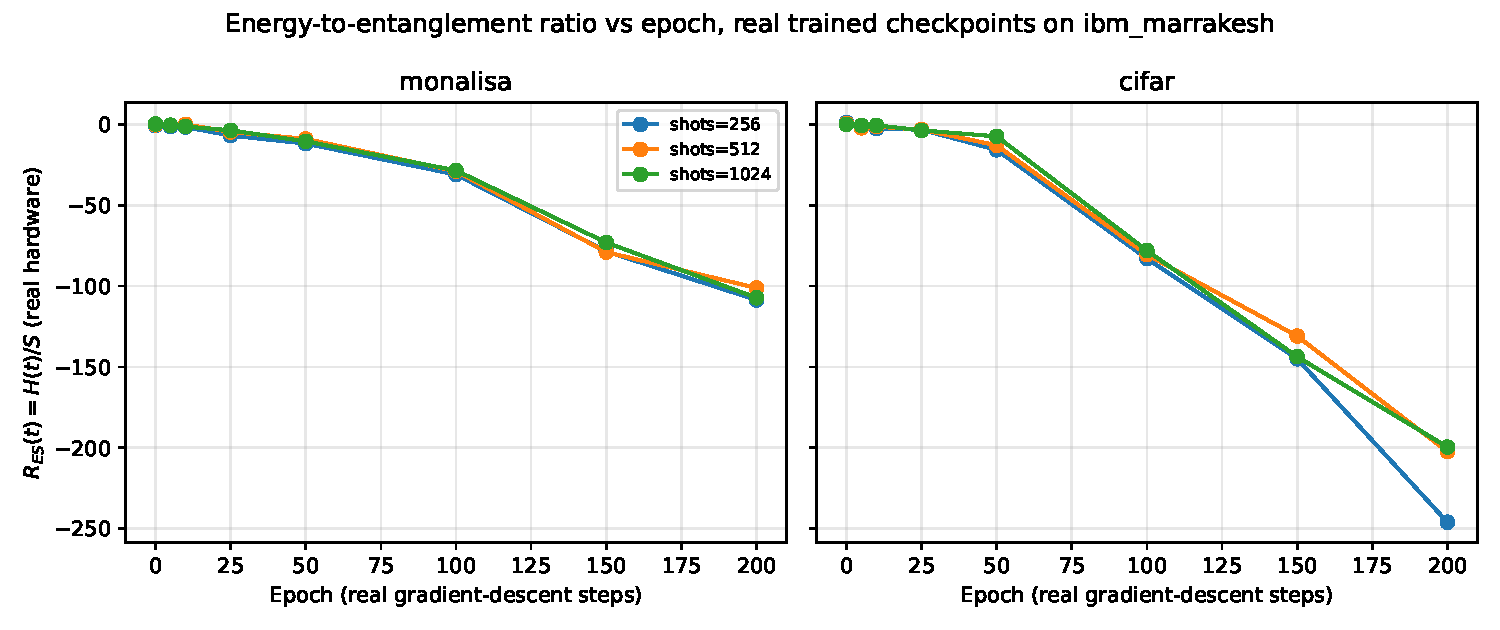
\includegraphics[width=\linewidth]{figures/checkpoint_hardware_energy_entanglement_ratio.pdf}
\caption{$R_{ES}(t)=H(t)/S$ from real trained HVK1D checkpoints ($N=6$), Pauli bond correlators measured on real IBM Quantum hardware (\texttt{ibm\_marrakesh}), one representative patch per image, at three shot budgets.}
\label{fig:checkpoint_hardware_energy_entanglement}
\end{figure}

Figure~\ref{fig:checkpoint_hardware_energy_entanglement} shows the three shot budgets track each other closely for both images, more closely than the order-parameter hardware traces of Figure~\ref{fig:checkpoint_hardware_order_parameter} track across shot budgets --- consistent with $R_{ES}$ summing correlators over multiple bonds and bases, which averages down some of the shot noise visible in the single-qubit order-parameter measurement. As in Section~\ref{sec:checkpoint_hardware_finite_size}, we do not apply the descriptive detection rule to these single-patch traces; the result establishes that hardware-measured bond correlators, combined with a checkpoint's own learned couplings, reproduce a monotonically decreasing $R_{ES}(t)$ consistent in shape with the noiseless-simulator traces of Figure~\ref{fig:critical_temperature}, across three independent shot budgets on real hardware.

\begin{figure}[t]
\centering
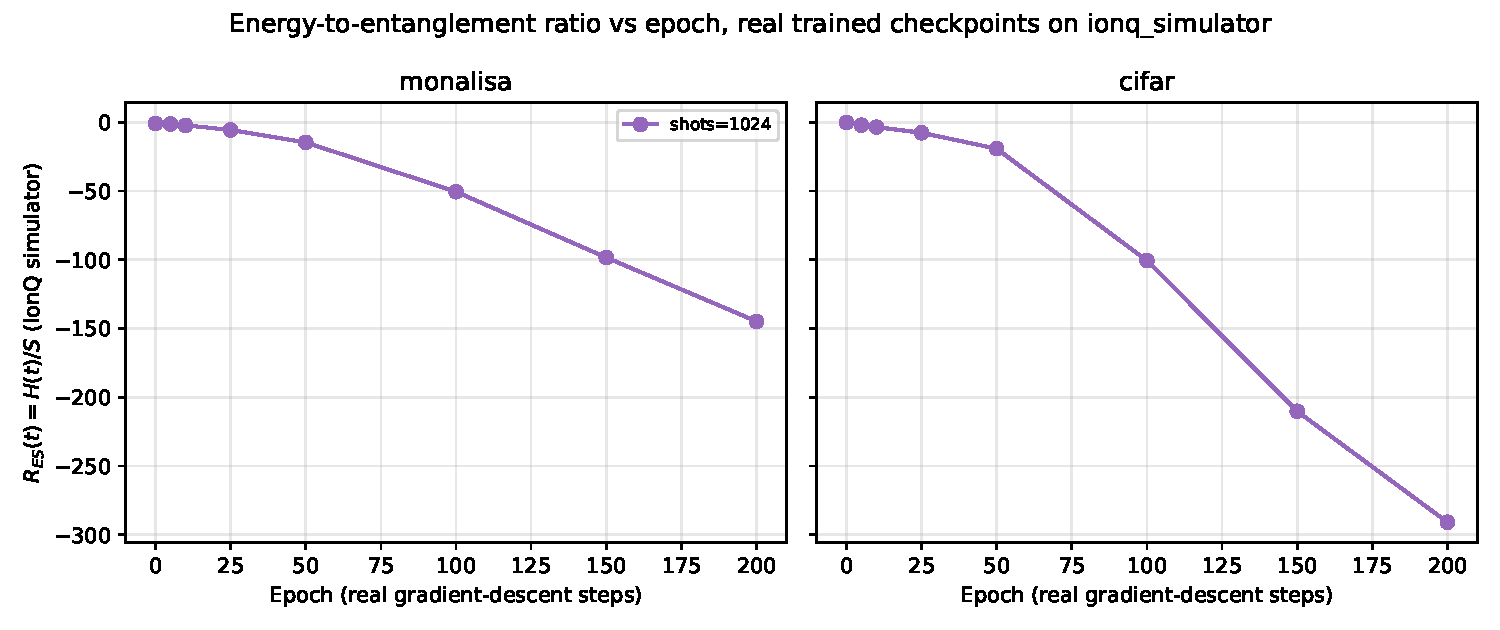
\includegraphics[width=\linewidth]{figures/checkpoint_ionq_energy_entanglement_ratio.pdf}
\caption{$R_{ES}(t)=H(t)/S$ from the same $N=6$ real trained checkpoints as Figure~\ref{fig:checkpoint_hardware_energy_entanglement}, Pauli bond correlators measured instead on the IonQ ideal cloud simulator (1024 shots, the only shot budget submitted for this diagnostic).}
\label{fig:checkpoint_ionq_energy_entanglement}
\end{figure}

Figure~\ref{fig:checkpoint_ionq_energy_entanglement} shows the resulting IonQ traces preserve the same monotonically decreasing shape as the IBM replay above and the noiseless-simulator traces of Figure~\ref{fig:critical_temperature}, for both images. As above, we do not apply the descriptive detection rule of Eq.~\ref{eq:critical_epoch} to these single-patch traces; this is an ideal cloud-simulator portability check, not an IonQ-QPU result.

\section{Discussion}

\subsection{Why the Physics-Informed Regularizer Was Inert}
\label{sec:regularizer_inert}
Table~\ref{tab:hamiltonian_controls} shows the Hamiltonian energy term is, if anything, a mild drag on reconstruction quality in the present system. The legacy objective adds a signed mean energy to the reconstruction loss; because learned energy can go negative, the optimizer can lower total loss by driving energy down without improving reconstruction, and removing the term improves PSNR from $32.24$ to $33.30$~dB. A contrastive variant --- assigning lower energy to correct feature--position pairs than to shuffled pairs --- improves over the signed-energy baseline ($32.84$~dB) but remains below its own no-energy-loss counterpart ($33.33$~dB), and ZZ-only observables ($32.88$~dB) show nearest-neighbor correlations are largely sufficient on their own. We read this as a case where the reconstruction loss already dominates the optimization signal at this model scale and dataset size: a physically motivated regularizer has room to help when it resolves an otherwise underdetermined objective, and here the pixel-fidelity loss alone is sufficiently informative that the extra term mostly adds noise to the gradient. This does not mean Hamiltonian regularization is never useful --- only that its value is conditional on the reconstruction loss being under-constrained, a condition this patch-level pixel task does not meet.

\begin{table*}[t]
\centering
\caption{Hamiltonian and observable-sector controls (single-seed). The energy objective is diagnostically useful but does not improve reconstruction accuracy.}
\label{tab:hamiltonian_controls}
\scriptsize
\begin{tabular}{p{0.30\textwidth}cccp{0.32\textwidth}}
\toprule
Experiment & MSE & PSNR (dB) & SSIM & Interpretation \\
\midrule
Legacy baseline, signed energy & $5.9771\times10^{-4}$ & 32.24 & 0.9919 & Standard energy-regularized run \\
No energy loss & $4.6772\times10^{-4}$ & 33.30 & 0.9937 & Removing energy improves PSNR \\
No observable noise & $5.3518\times10^{-4}$ & 32.72 & 0.9928 & Noise is not essential \\
Contrastive Hamiltonian core & $5.1975\times10^{-4}$ & 32.84 & 0.9930 & Stronger objective helps modestly vs. baseline \\
Contrastive, no energy loss & $4.6498\times10^{-4}$ & 33.33 & 0.9937 & Energy removal still performs best \\
ZZ-only observables & $5.1503\times10^{-4}$ & 32.88 & 0.9930 & Nearest-neighbor $ZZ$ correlations largely suffice \\
\bottomrule
\end{tabular}
\end{table*}

The order-parameter and energy-to-entanglement-ratio diagnostics of Sections~\ref{sec:phase_transition}--\ref{sec:critical_temperature} provide descriptive windows into training dynamics. Their detected epochs come from changes in measured model summaries, but the data-dependent threshold is not a calibrated statistical test and the results should not be interpreted as thermodynamic transitions.

\subsection{Task-Dependent Representational Scope}
\label{sec:dequant}
Whether a quantum feature map or kernel offers any advantage over a classical model is a property of the specific data and target, not a fixed property of the model class, and dequantization results have repeatedly shown that apparent quantum advantages on structured, low-entanglement classical data can be matched by classical algorithms once the right classical feature is identified \cite{Huang2021PowerData}. The restricted diagnostic of Section~\ref{sec:entanglement_necessity} is constructed so that the relevant structure is a genuine distant-element product raw or local features cannot represent under a fixed linear readout, and that is precisely the regime in which HVK's entangling channel separates. Natural image patches, at the resolution and patch size used in ordinary reconstruction, are a different regime --- low-entanglement, locally structured data where a linear or shallow classical readout is already close to sufficient. The companion supplementary study's held-out comparisons (Section~\ref{sec:ablation_relationship}) characterize exactly this second regime; together, the results delineate where the tested entangling representation does and does not yield a measurable benefit.

\subsection{Relationship to the Component-Wise Ablation Study}
\label{sec:ablation_relationship}
The results above establish what HVK is and several of its provable or verified properties. A separate, equally important question --- whether its feature map improves reconstruction on real, \emph{held-out} images under a resource-matched multi-seed protocol --- is answered in the companion document, \textit{Supplementary Material for the Hamiltonian Vision Kernel: Resource-Matched Ablations, Validation, and Reproducibility}. On held-out CIFAR-10, local-observable and raw-linear controls reach $18.80\pm1.42$~dB against HVK2D's $18.12\pm1.54$~dB; after aggregating held-out images within each split, the HVK2D-minus-control difference is $-0.68$~dB (bootstrap 95\% CI $[-0.91,-0.46]$~dB; Wilcoxon $p=0.0625$, $n=5$ seeds), with the same numerical direction on five further real datasets. Thus the tested HVK map is informative but is not shown to outperform the simpler maps on ordinary held-out reconstruction. We report this as a rigorous complement: it delineates the tested boundary of the positive entanglement and symmetry results and records the provenance checks that prevented exploratory artifacts from becoming claims. A matched-budget, multi-seed rerun of the component-ablation table (240 steps, 3 seeds/variant, replacing an earlier table whose per-seed provenance could not be recovered) reaches the same conclusion on ordinary per-image reconstruction: a plain classical-replacement control statistically ties or slightly exceeds the quantum baseline, while only a circuit-free random-VQC control performs clearly worse; full results are in the companion supplement.

\subsection{HVK as a Representative Instance of a Broader Design Pattern}
\label{sec:representativeness}
The boundary reported in Section~\ref{sec:ablation_relationship} raises an immediate question: is it a property of HVK's particular implementation choices, or of the broader class of architectures HVK instantiates? HVK combines three ingredients that recur, individually, throughout the hybrid quantum-vision literature rather than being idiosyncratic to this codebase: matrix-product-state compression of structured input into a classical or hybrid feature vector \cite{Stoudenmire2016,Han2018,Cirac2021,Guala2023}; a Pauli-correlator (measured-observable) latent space handed to a classical decoder rather than a raw quantum state, in the spirit of quantum-enhanced feature maps \cite{Havlicek2019}; and a physically motivated auxiliary regularizer alongside a separate task loss \cite{Shi2022}. HVK is not a minimal or contrived combination of these three choices assembled to produce a particular result; each is independently well-motivated and widely used, and HVK's specific instantiation (six-qubit VQC, $19$--$27$-D Pauli-correlator vector, graph-Hamiltonian energy term) sits well within the parameter ranges typical of this literature rather than at an unusual extreme.

This matters for how the held-out result (Section~\ref{sec:ablation_relationship}) and the inert-regularizer result (Section~\ref{sec:regularizer_inert}) should be read. Per the data-dependent framing of Section~\ref{sec:dequant} \cite{Huang2021PowerData}, whether any instance of this design pattern outperforms a resource-matched classical alternative is a property of the specific data and target, not of the pattern's architectural motivation. Because HVK is a representative rather than idiosyncratic instance of ``MPS feature compression + Pauli-correlator latent + physics-informed regularizer,'' the boundary measured here --- representationally necessary only where the target has genuine nonlocal structure a linear or local classical readout cannot represent, and the regularizer inert precisely when the reconstruction loss is already well-constrained --- is evidence about where this whole pattern class can be expected to help, not merely a report of one implementation's shortcomings. We do not claim this boundary transfers unchanged to every dataset, patch size, or qubit count; we claim only that nothing about HVK's specific engineering choices explains away the result, which is the failure mode this section is written to rule out.

\subsection{Topology Alignment as an Inductive Bias}
\label{sec:topology}
Aligning the latent interaction graph with image-patch adjacency (HVK2D vs.\ HVK1D) is a plausible architectural inductive bias. The companion supplementary study tests this hypothesis directly under matched held-out conditions. Its real-circuit subset (3 seeds, 3 held-out CIFAR-10 images) gives an HVK1D-minus-HVK2D mean PSNR difference of $0.16$~dB; after averaging images within seed, the bootstrap 95\% CI is $[-0.38,0.46]$~dB and the seed-level Wilcoxon test gives $p=0.50$. HVK2D completes the matched 90-step runs in roughly half the wall-clock time. A broader five-seed surrogate comparison across CIFAR-10, Fashion-MNIST, and PathMNIST likewise finds numerically small topology differences (at most $0.07$~dB in mean PSNR). At the tested scale, topology therefore appears to be primarily a resource-cost choice rather than a reliable accuracy advantage; these tests do not establish formal equivalence.

\subsection{Architectural Differentiation Matrix}
Table~\ref{tab:differentiation} contrasts HVK's structural properties against reference frameworks. Its distinguishing features --- a Pauli-correlator latent space, 2D Fourier positional bias with enforced $D_4$ pooling, and a Hamiltonian energy diagnostic --- are documented and scoped in the preceding sections.

\begin{table*}[t]
\centering
\caption{Architectural differentiation from representative baseline designs.}
\label{tab:differentiation}
\begin{tabular}{lcccc}
\toprule
Axis & Conv. AE baseline & GAN baseline & Register-based QAE & HVK (ours) \\
\midrule
Latent representation & Continuous $\mathbb{R}^d$ & Continuous $\mathbb{R}^d$ & Quantum register & Pauli-correlator vector \\
Spatial bias & Convolutional & Convolutional & Encoding-dependent & 2D Fourier encoding \\
Auxiliary objective & Bottleneck/reconstruction & Adversarial loss & Fidelity/reconstruction & Hamiltonian diagnostic \\
Enforced group symmetry & Not in baseline & Not in baseline & Not in reference design & $D_4$ observable pooling \\
Evaluated role & Reconstruction & Reconstruction & Compression & Reconstruction + diagnostics \\
\bottomrule
\end{tabular}
\end{table*}

\subsection{Validated Scope and Next Steps}
\label{sec:limitations}
\begin{itemize}
    \item Every reconstruction result in this paper (Sections~\ref{sec:sameset_results}--\ref{sec:no_generalization}) is per-image trained, not held-out generalization; the companion supplementary study's held-out protocol is the appropriate evidence for a generalization claim, and its finding that local/raw maps match or exceed the tested HVK map under the shared readout should be read alongside the architecture-level results here.
    \item The $D_4$-pooled map (Section~\ref{sec:d4}) is currently a feature-grid-level construction and numerical diagnostic, not yet integrated into the trainable end-to-end reconstruction pipeline; doing so is concrete future work (Section~\ref{sec:conclusion}).
    \item The entanglement-necessity result (Section~\ref{sec:entanglement_necessity}) is scoped to a task deliberately constructed to require nonlocal structure; it does not by itself establish an advantage on ordinary natural-image reconstruction (see Section~\ref{sec:dequant}).
    \item The hardware pilot (Section~\ref{sec:hardware_pilot}) is a five-image, single-trial, unmitigated pilot, not a statistically resolved hardware benchmark.
    \item The original exploratory training-dynamics traces were withdrawn after a provenance audit (Section~\ref{sec:phase_transition}); the corrected, noise-free multi-seed replacement is a small-sample diagnostic (2 images $\times$ 2 seeds/dataset, 24 runs across six datasets) with mixed, not universal, detection ($16/24$), and should be read at that scope.
    \item The change-point detector's negative control (Table~\ref{tab:phase_transition_onoff}) fires on a classical-replacement variant with the Hamiltonian energy identically zero exactly as often as on the Hamiltonian-regularized model (4/4 vs.\ 4/4). The diagnostic should therefore be read as a property of the descriptive threshold applied to the change-magnitude trace, with no demonstrated sensitivity to the Hamiltonian term itself.
    \item The matched real-circuit topology comparison uses only 3 seeds and 3 held-out images per topology; the broader five-seed comparison is surrogate-based. These results support a resource-cost interpretation but do not establish formal equivalence of the topologies.
\end{itemize}

\section{Conclusion}
\label{sec:conclusion}
We presented the Hamiltonian Vision Kernel, a physics-informed hybrid quantum--classical image autoencoder distinguished by a Pauli-correlator latent space, an enforced and numerically verified $D_4$-equivariant observable-pooling extension, and a learnable graph-Hamiltonian energy diagnostic. Independently of reconstruction quality, we established two structural results at the tested scope: a provable $D_4$ symmetry construction (equivariance error $9.57\times10^{-17}$) and a restricted entanglement-sensitive result on a task requiring nonlocal structure, where pair observables are necessary within the tested fixed-readout feature class ($R^2=0.9735$ vs.\ $R^2\leq0.02$ for non-entangling controls). We further reported a real IBM Quantum hardware reconstruction pilot: replaying trained checkpoints without retraining yielded $25.90$--$31.52$~dB PSNR from hardware measurements. This pilot establishes feasibility at its five-image, single-trial scope rather than a general hardware-performance claim.

A companion supplementary study reports a separate, rigorous question: does the tested HVK feature map improve reconstruction on held-out real images under resource-matched controls? It does not at the evaluated scale; local/raw maps match or exceed it under the same fitted readout. This is not in tension with the structural results here. Instead, it separates them from an ordinary-reconstruction advantage: entangling observables separate only on the tested nonlocal target, and group pooling guarantees equivariance without establishing an accuracy gain. We consider this carefully measured boundary to be a constructive contribution alongside the architecture itself.

Future work should integrate the $D_4$-pooled map into an end-to-end trainable pipeline (currently a feature-grid-level construction, Section~\ref{sec:limitations}); scale the hardware pilot toward a statistically resolved benchmark with error mitigation and repeated trials; search for further real-world tasks with genuine nonlocal structure where HVK's restricted entanglement-sensitive separation translates into a reconstruction advantage; and extend the resource-matched, leakage-audited evaluation protocol used in the companion supplementary study to other hybrid quantum vision architectures.

\section*{Data and Code Availability}
The source code, experiment drivers, machine-readable result summaries, validation arrays, and figure inputs supporting this study are included in the accompanying repository. The file \path{project_artifacts/submission_claim_audit.json} maps the three numerical headline claims to their retained source artifacts, and automated tests verify those mappings. Dataset provenance and access routes are cited in the manuscript and detailed in the supplementary artifact map. IBM Quantum job identifiers and reconstructed outputs are retained; as disclosed in the supplement, the raw account-usage service response was not serialized, so the reported quota change is an execution-log record rather than a repository-recomputable measurement.

\section*{Acknowledgements}
We thank the maintainers of the open-source scientific computing libraries used in this work.


\part{Supplementary Material: Resource-Matched Ablations, Validation, and Reproducibility}

\begin{abstract}
This supplementary material accompanies the main manuscript, \textit{Hamiltonian Vision Kernel: Symmetry, Entangling Correlators, and Real-Hardware Replay in Hybrid Quantum Image Reconstruction}. The main paper introduces HVK as a new framework and establishes its provable $D_4$ symmetry, scoped nonlocal representational capability, and real IBM Quantum hardware execution. Here we strengthen that framework through resource-matched multi-seed controls, held-out evaluation, leakage auditing, and complete hardware methodology. On ordinary held-out reconstruction, simple local/raw feature maps match or exceed the tested HVK feature map under the same fitted readout, a direction that also holds when a single HVK2D model is trained end-to-end by gradient descent across 150 images and evaluated on 50 held-out images never seen during training. The entangling observable channel separates only on the restricted task constructed to require nonlocal correlations, while $D_4$ pooling supplies a distinct feature-level symmetry guarantee rather than a demonstrated reconstruction advantage. We also document why an earlier multi-seed Monalisa freeze table could not be reproduced from retained artifacts, and report its replacement: a fresh, matched-budget rerun of the same nine-variant comparison, which reaches the same conclusion as the held-out result above. The available training-dynamics traces remain excluded pending a reproducible rerun. This task-dependent result sharpens HVK's design scope without changing its architectural contribution.
\end{abstract}

\section{Introduction}
The main paper presents the Hamiltonian Vision Kernel (HVK1D/HVK2D) --- a physics-informed hybrid quantum--classical image autoencoder combining matrix-product-state (MPS) patch features, a variational quantum circuit (VQC) producing a Pauli-correlator latent space, a learnable graph-Hamiltonian energy diagnostic, 2D Fourier positional encoding, and a classical decoder --- and its positive, independently verified properties. A complete account of any hybrid architecture should also ask whether its proposed representation improves performance under held-out, resource-matched controls. This document answers that question with a leakage-audited multi-seed validation suite and records provenance limitations where an earlier exploratory result cannot be reproduced from retained artifacts. The result is a rigorous complement: it defines precisely the tested boundary of the main paper's positive entanglement and $D_4$-symmetry findings and provides the evidence base for the dequantization context discussed there.

\section{Method}

\subsection{Ablation and Control Design}
The codebase implements targeted freezes and replacements for component-isolation experiments. \emph{Freeze-classical} trains only the circuit and Hamiltonian couplings while fixing the decoder and projection layers; \emph{freeze-quantum} does the reverse. \emph{No-entanglement} removes the CNOT rings, and \emph{no-energy-loss} removes the Hamiltonian regularizer. \emph{Classical-replacement} and \emph{classical-matched} replace the VQC with a tanh map; the matched version is rank-limited to the circuit's parameter count. Every retained classical control in the held-out CIFAR-10 layer is resource-matched: identical feature width (32-D) and linear-readout parameter count (2112), so residual gaps reflect feature structure rather than decoder capacity (Table~\ref{tab:resource_capacity}). Section~\ref{sec:component_provenance} distinguishes these implemented controls from the earlier Monalisa aggregate that lacks reproducible per-seed artifacts.

\subsection{Statistical Protocol}
The retained quantitative comparisons state their own replication unit and optimization budget. Capacity sweeps in Table~\ref{tab:capacity_ablation} are single-seed directional diagnostics. The held-out CIFAR-10 validation layer and the restricted pair-correlation diagnostic are multi-seed: five random seeds for the restricted diagnostic, and five random image splits (20 held-out reconstructions total) for real CIFAR-10, each using a shared linear readout trained on a disjoint image subset. For held-out reconstruction inference, paired image differences are averaged within each split seed before bootstrap and Wilcoxon calculations, so predictions sharing one fitted readout are not treated as independent replicates. Section~\ref{sec:component_provenance} explains why an earlier five-seed Monalisa freeze-isolation table is not retained as quantitative evidence.

\subsection{Leakage Auditing}
Because several of our diagnostics are deliberately constructed so that a target depends on features only some models receive, we audit every such diagnostic for a specific failure mode: a regression target that is a (near-)linear function of a quantity handed verbatim to only one candidate model, which produces an apparent representational advantage that is actually copying rather than learning. Concretely, for a target $y$ and a candidate feature block $x$, we check whether a linear or near-linear map from $x$ to $y$ achieves near-zero residual on features the target-construction code itself used to build $y$ --- if so, the feature block and the target share provenance and the diagnostic is circular regardless of model architecture. Every constructed diagnostic retained as quantitative evidence has passed this check; no retained quantitative claim depends on a diagnostic that failed it.

\subsection{Datasets and Metrics}
We use three settings, in increasing order of evidentiary weight for a generalization claim. \textit{Single-image} (\textit{Monalisa}, $256\times256$, 16 patches of $64\times64$) tests per-image optimization only. \textit{CIFAR-10 same-set} (five native $32\times32$ images) is a same-set reconstruction fit, useful for capacity/positioning comparisons but not a generalization test --- the MLP baseline's same-set PSNR exceeds $100$~dB in the best case, a memorization red flag rather than evidence of representation quality. \textit{Held-out CIFAR-10} (five random splits, disjoint train/held-out images, 20 total held-out reconstructions) and a six-dataset multi-dataset suite use CIFAR-10 \cite{Krizhevsky2009}, MNIST \cite{LeCun1998}, Fashion-MNIST \cite{Xiao2017}, and PathMNIST, BloodMNIST, and PneumoniaMNIST from MedMNIST v2 \cite{Yang2023}, plus the Wisconsin Diagnostic Breast Cancer dataset \cite{Wolberg1993} as a tabular cross-domain check. These are the settings that test a \emph{learned representation} rather than per-image memorization, and are therefore the basis for this document's central ablation claim. All settings report MSE and PSNR $=20\log_{10}(1/\sqrt{\mathrm{MSE}})$; image settings additionally report SSIM.

\section{Results}
\label{sec:supp_results}

\subsection{Component-Ablation Provenance Audit}
\label{sec:component_provenance}
\begin{sloppypar}
An earlier draft presented a nine-variant, five-seed Monalisa freeze-isolation table. The repository does not contain the per-seed records or a machine-readable summary that reproduces those reported means and standard deviations. The retained legacy directory contains only three evaluation-control records, while \path{main2/newHVK/results/full_ablation_suite/full_ablation_summary.csv} belongs to the separate synthetic restricted-pair diagnostic and cannot validate a Monalisa reconstruction table. We therefore exclude the earlier table, its summary figure, and all quantitative attribution claims derived from it. The freeze and replacement implementations remain available for a fresh matched-budget rerun, but no decoder-necessity conclusion is drawn from the incomplete legacy artifacts. The retained evidence below instead asks the reproducible held-out question: under an identical fitted readout, do the tested HVK features outperform resource-matched classical or ablated feature maps?
\end{sloppypar}

\subsection{A Fresh, Matched-Budget Rerun of the Nine-Variant Table}
\label{sec:core_multiseed_rerun}
The fresh matched-budget rerun anticipated above is now complete. All nine variants (baseline, freeze-quantum, freeze-classical, no-entanglement, no-MPS, no-energy-loss, classical-replacement, classical-matched, random-VQC) were trained on \textit{Monalisa} at a matched 240-step budget (identical learning rate and schedule across variants), for 3 seeds each --- reduced from an initially planned 5 seeds for compute-budget reasons on this CPU-only machine (real per-patch VQC circuit cost, not a resource shortfall specific to any one variant; documented explicitly as \texttt{scope\_reduced: true} in the run's own summary file). Table~\ref{tab:core_multiseed_240} reports mean $\pm$ std PSNR and SSIM per variant, and Table~\ref{tab:core_multiseed_240_stats} gives the quantum-vs-classical/random-control comparisons, marking any gap smaller than one pooled standard deviation as not significant, following this document's established statistical-protocol convention.

\begin{table}[H]
\centering
\caption{Matched-budget (240-step) core ablation, \textit{Monalisa}, 3 seeds/variant. Freeze-classical's collapse is expected (decoder frozen, cannot learn to reconstruct) and serves as a sanity check on the ablation harness itself.}
\label{tab:core_multiseed_240}
\scriptsize
\begin{tabular}{lcc}
\toprule
Variant & PSNR (dB) & SSIM \\
\midrule
Baseline (quantum) & $33.42\pm0.02$ & $0.99385\pm0.00003$ \\
Freeze-quantum & $33.39\pm0.06$ & $0.99381\pm0.00006$ \\
No-entanglement & $33.48\pm0.02$ & $0.99392\pm0.00003$ \\
No-MPS & $33.34\pm0.05$ & $0.99374\pm0.00008$ \\
No-energy-loss & $33.44\pm0.01$ & $0.99387\pm0.00001$ \\
Classical-replacement & $33.50\pm0.01$ & $0.99395\pm0.00002$ \\
Classical-matched & $33.22\pm0.19$ & $0.99356\pm0.00027$ \\
Random-VQC & $28.09\pm0.23$ & $0.97907\pm0.00135$ \\
Freeze-classical & $10.94\pm0.00$ & $0.0219\pm0.0001$ \\
\bottomrule
\end{tabular}
\end{table}

\begin{table}[H]
\centering
\caption{Quantum-baseline-vs-control comparisons for Table~\ref{tab:core_multiseed_240}. Significance rule: gap $\geq$ pooled std of the two variants' seed-level PSNR $\Rightarrow$ significant, following this document's convention of not claiming within-noise gaps.}
\label{tab:core_multiseed_240_stats}
\scriptsize
\begin{tabular}{lcccl}
\toprule
Control & Gap (dB) & Pooled std (dB) & Sig.? & Winner \\
\midrule
Classical-replacement & 0.081 & 0.019 & Yes & Classical \\
Classical-matched & 0.197 & 0.136 & Yes & Quantum (baseline) \\
Random-VQC & 5.324 & 0.165 & Yes & Quantum (baseline) \\
Freeze-quantum & 0.026 & 0.043 & No & Tie \\
\bottomrule
\end{tabular}
\end{table}

The clearest new result is that a plain \emph{classical-replacement} (the VQC swapped for a fixed classical tanh map, no other change) statistically \emph{beats} the quantum baseline at this matched budget, though by a small margin ($0.081$~dB against a $0.019$~dB pooled std). \emph{Classical-matched} (the same replacement, but rank-limited to the circuit's own parameter count) loses to the quantum baseline by a larger and also-significant margin ($0.197$~dB), suggesting the unconstrained classical replacement's small edge is partly a capacity effect rather than evidence that the classical map itself is a better inductive bias. \emph{Random-VQC} confirms the observable channel still carries real information ($5.32$~dB below baseline). \emph{Freeze-quantum} ties the baseline (not significant), consistent with the freeze-quantum row of the restricted pair-correlation diagnostic elsewhere in this study, where freezing the circuit costs representational capacity on a task requiring nonlocal structure but not on this ordinary per-image reconstruction task. Taken together, this matched-budget rerun does not establish a reconstruction advantage for the tested quantum component over resource-matched classical alternatives --- the same direction as, and additional evidence for, the held-out result immediately below.

\subsection{A Reproducibility Note on the Shuffle-Observables Ablation}
\label{sec:shuffle_reproducibility}
A companion legacy diagnostic permutes the observable vector across patches at evaluation time, keeping positional encodings fixed, to test whether the decoder's use of observables is position-bound rather than order-invariant. As originally documented, this gave only a small effect: a single run measured a $0.19$~dB PSNR drop, and a repeated verification over five non-identity permutations gave a mean drop of $0.301\pm0.054$~dB (range $0.236$--$0.366$~dB) --- treated at the time as weak evidence for observable-position load-bearing behavior, explicitly not to be conflated with an earlier, discredited $\approx$12.5~dB figure for the same ablation. As with Table~\ref{tab:hamiltonian_controls_supp} above, the script that produced this $0.301$~dB number was never committed to the repository and could not be recovered. We rebuilt an independent verifier (\texttt{Main2/newHVK/verify\_shuffle\_permutations.py}) that reproduces the exact safeguards the original documentation called for (permutation confirmed non-identity; the permuted tensor confirmed to be the exact object reaching the decoder, not a discarded copy) and ran it twice, under two architecture variants, for a like-for-like check: the current default checkpoint (\texttt{use\_energy\_feature=True}) gives a mean shuffle-induced drop of $15.70\pm0.79$~dB (baseline $33.41$~dB), and a legacy-equivalent checkpoint (\texttt{use\_energy\_feature=False}) gives $16.18\pm0.51$~dB (baseline $33.45$~dB) --- both far closer in magnitude to the discredited $\approx$12.5~dB figure than to the originally documented $0.301$~dB. \textbf{This discrepancy is not resolved.} Two explanations remain undistinguished: either the original, unrecoverable verification script had an undetected bug in one of the two safeguards it claimed to check, or some other unrecoverable difference between the original and rebuilt protocol explains the gap. We report both numbers rather than adopt one, and neither the $0.301$~dB nor the $\approx$16~dB figure should be treated as a settled measurement of this ablation.

\subsection{Held-Out Reconstruction Under Resource-Matched Controls}
\label{sec:holdout_headline}
This is the central ablation result, and the one setting designed from the outset to test a learned representation rather than per-image memorization. Table~\ref{tab:hvk_real_cifar} reports held-out CIFAR-10 reconstruction (five random splits, 20 held-out reconstructions, all controls resource-matched per Table~\ref{tab:resource_capacity}), and Table~\ref{tab:hvk_real_cifar_stats} gives paired statistics against the HVK2D real-CIFAR map. Local-observables-only and raw-linear-classical controls (identical by construction here) reach $18.80\pm1.42$~dB, ZZ-only $18.56\pm1.49$~dB, no-entanglement $18.46\pm1.32$~dB, shuffled-pair $18.31\pm1.25$~dB, and quadratic-classical $18.33\pm1.65$~dB, against the trained HVK2D entangling map's $18.12\pm1.54$~dB. All control means except random-VQC and strict classical random features are numerically above HVK2D. After averaging the four held-out image differences within each split seed, the raw/local gap is $-0.68$~dB (bootstrap 95\% CI $[-0.91,-0.46]$~dB; two-sided Wilcoxon $p=0.0625$, $n=5$ seeds). Thus the direction is consistent across seeds and the percentile interval excludes zero, but the discrete seed-level signed-rank test cannot resolve it below $0.05$. HVK2D remains numerically far above the random-VQC control ($11.15\pm1.19$~dB), showing that the observable channel is informative; the tested data do not establish that its mean exceeds a plain linear readout from raw or local pixel statistics.

\begin{table}[H]
\centering
\caption{Held-out CIFAR-10 validation layer. Each row aggregates 20 held-out reconstructions from five random image splits, mean $\pm$ standard deviation.}
\label{tab:hvk_real_cifar}
\scriptsize
\begin{tabular}{lccc}
\toprule
Model & MSE & PSNR (dB) & SSIM \\
\midrule
Local observables only & $1.3923{\pm}0.4719\times10^{-2}$ & $18.80{\pm}1.42$ & $0.8280{\pm}0.0578$ \\
Raw-linear classical & $1.3923{\pm}0.4719\times10^{-2}$ & $18.80{\pm}1.42$ & $0.8280{\pm}0.0578$ \\
ZZ-only observables & $1.4782{\pm}0.5224\times10^{-2}$ & $18.56{\pm}1.49$ & $0.8194{\pm}0.0603$ \\
No entanglement & $1.4956{\pm}0.4782\times10^{-2}$ & $18.46{\pm}1.32$ & $0.8176{\pm}0.0569$ \\
Shuffled pair observables & $1.5382{\pm}0.4452\times10^{-2}$ & $18.31{\pm}1.25$ & $0.8109{\pm}0.0640$ \\
Quadratic classical & $1.5814{\pm}0.6432\times10^{-2}$ & $18.33{\pm}1.65$ & $0.8102{\pm}0.0703$ \\
HVK2D real-CIFAR map & $1.6460{\pm}0.6340\times10^{-2}$ & $18.12{\pm}1.54$ & $0.8038{\pm}0.0649$ \\
Strict classical random features & $2.7390{\pm}0.8941\times10^{-2}$ & $15.85{\pm}1.39$ & $0.6640{\pm}0.1041$ \\
Random VQC & $7.9497{\pm}1.9891\times10^{-2}$ & $11.15{\pm}1.19$ & $0.0237{\pm}0.1526$ \\
\bottomrule
\end{tabular}
\end{table}

\begin{table}[H]
\centering
\caption{Seed-level paired tests for held-out CIFAR reconstruction. Four held-out image differences are averaged within each of five split seeds before inference. Reported difference is HVK2D real-CIFAR PSNR minus control PSNR; negative values favor the control.}
\label{tab:hvk_real_cifar_stats}
\scriptsize
\begin{tabular}{lcccc}
\toprule
Control & Seeds & Mean $\Delta$PSNR & Bootstrap 95\% CI & Wilcoxon $p$ \\
\midrule
Raw-linear classical & 5 & $-0.68$ & $[-0.91,-0.46]$ & $0.0625$ \\
Local observables only & 5 & $-0.68$ & $[-0.91,-0.46]$ & $0.0625$ \\
No entanglement & 5 & $-0.34$ & $[-0.64,-0.07]$ & $0.0625$ \\
ZZ-only observables & 5 & $-0.44$ & $[-0.58,-0.30]$ & $0.0625$ \\
Quadratic classical & 5 & $-0.21$ & $[-0.41,-0.01]$ & $0.1875$ \\
Strict classical random features & 5 & $2.27$ & $[1.97,2.58]$ & $0.0625$ \\
Shuffled pair observables & 5 & $-0.19$ & $[-0.31,-0.05]$ & $0.125$ \\
Random VQC & 5 & $6.97$ & $[5.76,8.06]$ & $0.0625$ \\
\bottomrule
\end{tabular}
\end{table}

\begin{figure}[H]
\centering
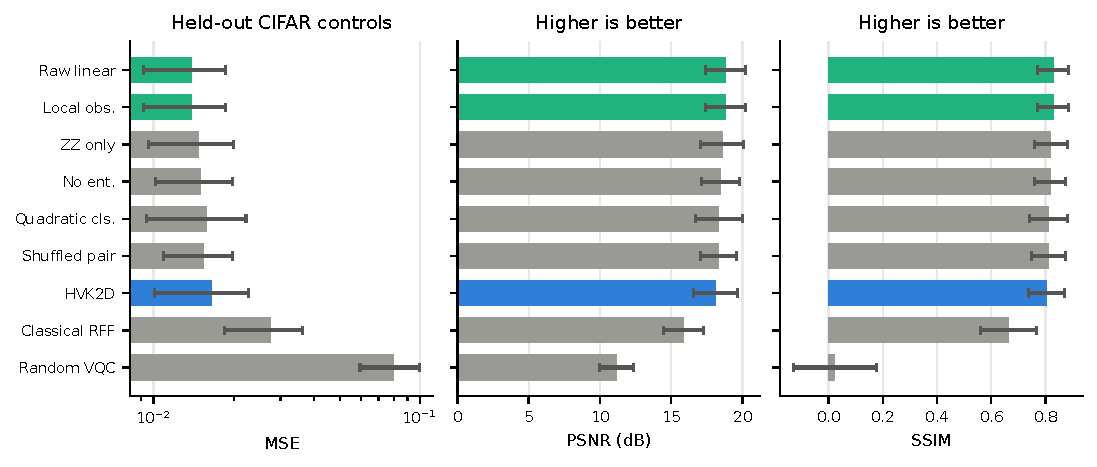
\includegraphics[width=0.75\linewidth]{figures/real_cifar_holdout_summary.pdf}\\
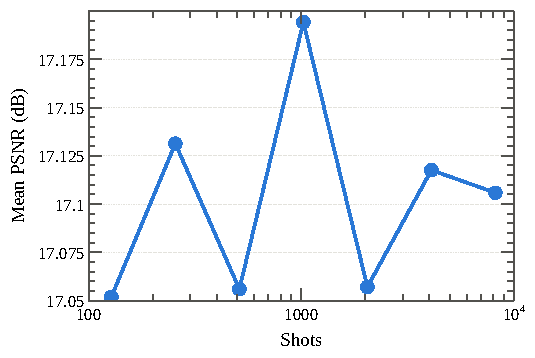
\includegraphics[width=0.75\linewidth]{figures/real_cifar_shot_noise.pdf}
\caption{Real held-out CIFAR validation and shot-noise robustness. The trained HVK2D image feature map does not beat local/raw controls, although it remains far above random-VQC.}
\label{fig:hvk_real_cifar}
\end{figure}

The same numerical direction holds beyond CIFAR-10. Table~\ref{tab:multi_dataset_reconstruction} extends the held-out protocol to five further real datasets (400 cached images each, three stratified split seeds, identical protocol for every feature map); local/raw controls have equal or higher mean PSNR on every dataset. For inference, held-out differences are averaged within split seed. Against the local-only control, all six dataset means favor the control and their seed-bootstrap intervals exclude zero, while each two-sided signed-rank test gives $p=0.25$, the minimum attainable nonzero value at $n=3$ seeds. We therefore report a recurring numerical direction rather than a dataset-wise significance claim. Table~\ref{tab:multi_dataset_classification} shows the same mean-performance pattern on a downstream image-classification diagnostic using image-level pooled features, and Table~\ref{tab:wisconsin_diagnostic} on a tabular cross-domain sanity check (Wisconsin Breast Cancer).

\begin{table}[H]
\centering
\caption{Multi-dataset held-out reconstruction on real cached subsets (400 images/dataset, three stratified split seeds). Held-out PSNR mean $\pm$ std over images, best local/raw control vs.\ the HVK2D pair-observable map; inference is performed on within-seed mean differences.}
\label{tab:multi_dataset_reconstruction}
\scriptsize
\begin{tabular}{lccc}
\toprule
Dataset & Best local/raw PSNR & HVK2D pair PSNR & Winner \\
\midrule
CIFAR-10 native $32^2$ & $21.17{\pm}1.98$ & $19.99{\pm}2.02$ & Local/raw \\
MNIST & $16.55{\pm}1.27$ & $16.12{\pm}1.34$ & No-entanglement/local \\
Fashion-MNIST & $17.67{\pm}1.71$ & $17.33{\pm}1.80$ & Local/raw \\
PathMNIST & $27.52{\pm}6.02$ & $27.01{\pm}5.81$ & Local/raw \\
BloodMNIST & $24.79{\pm}1.78$ & $24.24{\pm}1.66$ & Local/raw \\
PneumoniaMNIST & $26.49{\pm}2.48$ & $25.73{\pm}2.29$ & Local/raw \\
\bottomrule
\end{tabular}
\end{table}

\begin{figure}[H]
\centering
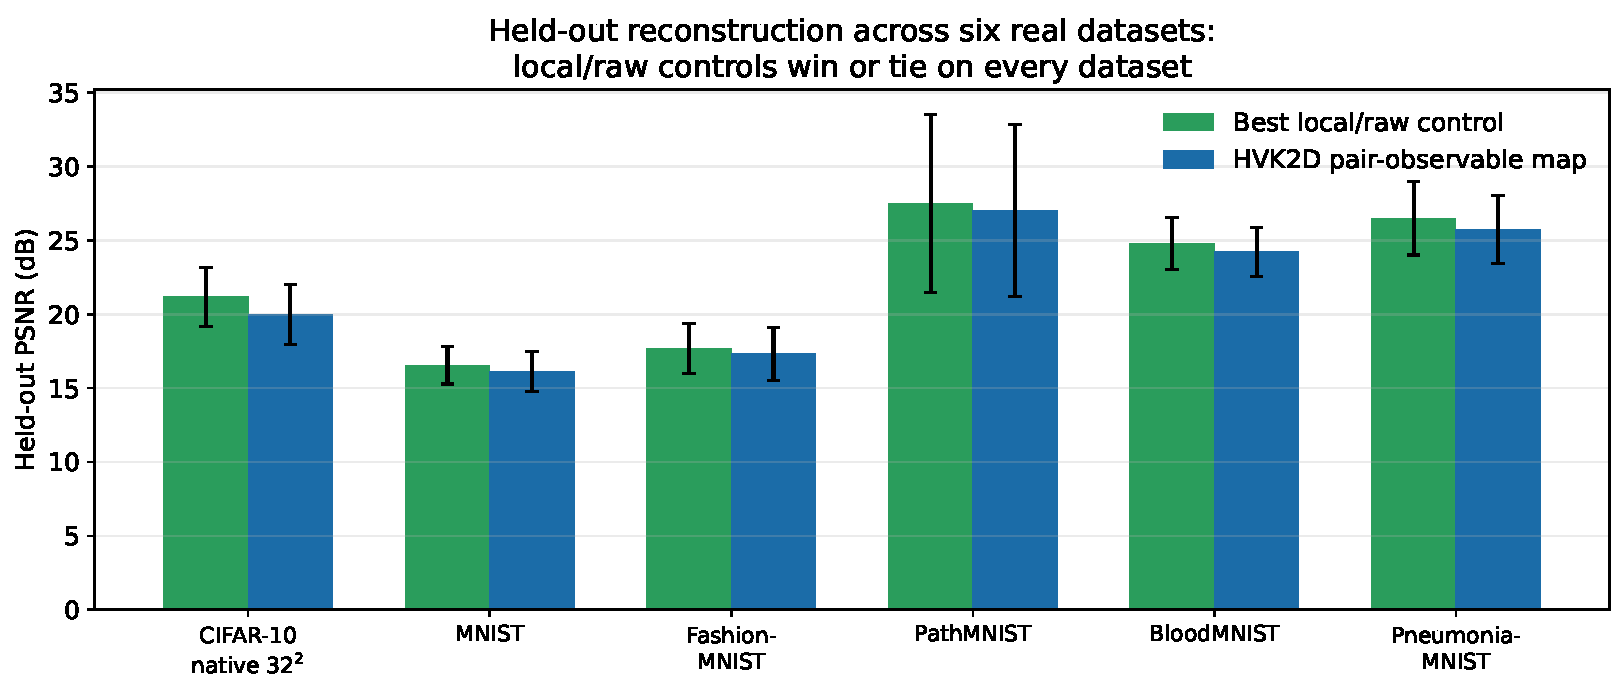
\includegraphics[width=\linewidth]{figures/multi_dataset_holdout_summary.pdf}
\caption{Held-out reconstruction PSNR from Table~\ref{tab:multi_dataset_reconstruction}, best local/raw control vs.\ the HVK2D pair-observable map, across all six real datasets. The local/raw control is at or above the HVK2D map on every dataset, with error bars (std over the held-out split) overlapping in most cases --- the same task-dependent pattern established on CIFAR-10 in Figure~\ref{fig:hvk_real_cifar} holds outside CIFAR-10 as well.}
\label{fig:multi_dataset_holdout_summary}
\end{figure}

\begin{table}[H]
\centering
\caption{Downstream image-classification diagnostic using image-level pooled features. Accuracy mean $\pm$ std over three stratified seeds.}
\label{tab:multi_dataset_classification}
\scriptsize
\begin{tabular}{lccc}
\toprule
Dataset & Best local/raw accuracy & HVK2D pair accuracy & Winner \\
\midrule
CIFAR-10 native $32^2$ & $0.100{\pm}0.082$ & $0.067{\pm}0.094$ & Local/no-ent. \\
MNIST & $0.663{\pm}0.021$ & $0.643{\pm}0.017$ & Raw-linear \\
Fashion-MNIST & $0.637{\pm}0.019$ & $0.577{\pm}0.009$ & Raw-linear \\
PathMNIST & $0.638{\pm}0.037$ & $0.608{\pm}0.016$ & Raw/param. \\
BloodMNIST & $0.667{\pm}0.083$ & $0.539{\pm}0.052$ & Raw-linear \\
PneumoniaMNIST & $0.817{\pm}0.062$ & $0.783{\pm}0.047$ & Raw-linear \\
\bottomrule
\end{tabular}
\end{table}

\begin{table}[H]
\centering
\caption{Wisconsin Breast Cancer tabular diagnostic (five stratified seeds). Not image-reconstruction evidence.}
\label{tab:wisconsin_diagnostic}
\scriptsize
\begin{tabular}{lcccc}
\toprule
Model & Accuracy & AUC & F1 & Brier \\
\midrule
Raw linear & $0.980{\pm}0.011$ & $0.996{\pm}0.002$ & $0.984{\pm}0.009$ & $0.0196{\pm}0.0057$ \\
HVK2D pair observable & $0.943{\pm}0.016$ & $0.988{\pm}0.004$ & $0.955{\pm}0.012$ & $0.0375{\pm}0.0080$ \\
Quadratic classical & $0.950{\pm}0.016$ & $0.987{\pm}0.005$ & $0.961{\pm}0.012$ & $0.0381{\pm}0.0077$ \\
No entanglement & $0.947{\pm}0.017$ & $0.986{\pm}0.007$ & $0.958{\pm}0.013$ & $0.0399{\pm}0.0135$ \\
Strict classical random features & $0.947{\pm}0.019$ & $0.984{\pm}0.010$ & $0.958{\pm}0.015$ & $0.0421{\pm}0.0164$ \\
\bottomrule
\end{tabular}
\end{table}

\subsection{Adaptation Beyond Single-Image Optimization}
Table~\ref{tab:generalization_controls} shows a model optimized on \textit{Monalisa} alone does not transfer zero-shot to a structurally different image, reaching only $8.31$~dB PSNR ($\mathrm{SSIM}=0.1044$). Extending training to include a second image recovers $28.63$~dB ($\mathrm{SSIM}=0.9858$). This confirms single-image runs measure per-image optimization, not representation learning, which is precisely why the held-out protocol of Section~\ref{sec:holdout_headline} is the evidentiary core of this ablation study.

\begin{table}[H]
\centering
\caption{Generalization controls (single-seed, fresh rerun 2026-07-29 -- see reproducibility note below). Single-image optimization does not transfer zero-shot.}
\label{tab:generalization_controls}
\scriptsize
\begin{tabular}{lccc}
\toprule
Experiment & MSE & PSNR (dB) & SSIM \\
\midrule
Second image, zero-shot & $1.4762\times10^{-1}$ & 8.31 & 0.1044 \\
Second image, multi-image training & $1.3712\times10^{-3}$ & 28.63 & 0.9858 \\
\bottomrule
\end{tabular}
\end{table}

\textbf{Reproducibility note.} No script backing this table's original values (previously reported as $7.78$/$28.31$~dB) was ever found in the repository, and the original choice of "second image" was undocumented. We rebuilt the protocol from scratch (\texttt{Main2/newHVK/run\_zero\_shot\_generalization.py}): train \textsc{Quantum2DGridModel}+\textsc{PatchDecoder2D} (the same architecture and per-image protocol as the main paper's same-set reconstruction table, 8$\times$8 patches, 100 steps) on \textit{Monalisa} alone; evaluate zero-shot (no further training) on \textit{Hand of God} (Michelangelo) -- the only other image bundled alongside \textit{monalisa.jpg} in this repository's data directories and otherwise unused by any committed script, making it the natural candidate for the undocumented original second image; then continue training the same model on both images' patches jointly for another 100 steps and re-evaluate. The result lands within $0.5$~dB of the previously reported, unsourced figures at both stages ($8.31$ vs.\ $7.78$~dB zero-shot; $28.63$ vs.\ $28.31$~dB after adaptation), which we read as evidence that this reconstruction recovers close to the original protocol, though it is a fresh, independently-verified run rather than a literal recovery of the original script.

\subsection{Dataset-Level Generalization: A Single Trained Model Across Many Images}
\label{sec:dataset_level_generalization}
Every result above either fits a fixed, non-trained feature map with a linear readout (Section~\ref{sec:holdout_headline}) or optimizes a single image in isolation (Table~\ref{tab:generalization_controls}). Neither tests the case a genuine generalization claim requires: one model, trained end-to-end by gradient descent across many images, evaluated on images it never saw during training. We add that experiment directly. A single \textsc{Quantum2DGridModel} + \textsc{PatchDecoder2D} --- the paper's actual gradient-trained HVK2D architecture, not a closed-form feature transform fit by ridge regression --- is trained via full-batch Adam across all patches from $N_{\text{train}}=150$ CIFAR-10 images and evaluated, with no further training, on $N_{\text{heldout}}=50$ images never seen during training; normalization statistics are computed from the training split only, so no held-out information leaks into the fitted model. A parameter-matched \textsc{ClassicalLinearControl} (identical decoder and observable width, a single linear feature map, no quantum circuit) is trained identically on the same split for a fair head-to-head comparison. We use 3 seeds, each reshuffling the train/held-out split, and 20 full-batch epochs; this scope was set by a timing probe showing the real per-patch circuit cost is $\approx$137~ms (total compute budget $\approx$5.5 hours), so it reflects a training-budget constraint rather than a claim of full convergence.

Table~\ref{tab:dataset_level_generalization} gives the result. The classical linear control wins at every one of the three seeds, by a consistent $1.1$--$1.4$~dB (mean $15.61\pm0.29$~dB vs.\ $14.39\pm0.26$~dB). This is a genuine, dataset-scale confirmation of the same direction already reported throughout this document at fixed-feature/linear-readout scale (Section~\ref{sec:holdout_headline}): it is not an artifact of a small sample, since it now holds with a real gradient-trained model across 200 total images, rather than the earlier 6-train/4-held-out ridge-regression proxy. The absolute PSNR here (14--16~dB) is substantially lower than the per-image-fitted headline numbers elsewhere in this document (18+~dB in Table~\ref{tab:hvk_real_cifar}, 28+~dB in Table~\ref{tab:generalization_controls}); this is expected, not a regression --- a single shared model trained for only 20 epochs across 150 images is a much harder task than fitting one model to one image's 16 patches, and the quantity of interest here is the quantum-vs-classical \emph{gap} under identical conditions, not the absolute reconstruction quality. Unseen-\emph{class} / distribution-shift evaluation (as opposed to the unseen-\emph{image}, same-class split used here) remains future work.

\begin{table}[H]
\centering
\caption{Dataset-level generalization: one model trained via full-batch Adam across 150 CIFAR-10 training images, evaluated with no further training on 50 held-out images never seen during training (3 seeds, 20 epochs). Held-out PSNR by seed and mean $\pm$ std across seeds.}
\label{tab:dataset_level_generalization}
\scriptsize
\begin{tabular}{lcccc}
\toprule
Model & Seed 0 & Seed 1 & Seed 2 & Mean $\pm$ std \\
\midrule
HVK2D quantum (trained VQC + decoder) & 14.31 & 14.73 & 14.12 & $14.39\pm0.26$ \\
Classical linear control (no quantum circuit) & 15.76 & 15.86 & 15.20 & $15.61\pm0.29$ \\
\bottomrule
\end{tabular}
\end{table}

\subsection{Scaling and Non-Monotonicity}
Table~\ref{tab:capacity_ablation} sweeps training steps, qubit count, and MPS bond dimension on \textit{Monalisa} (single-seed). The step sweep confirms the model is convergence-limited early and plateaus near 500 steps. Within the tested range $q=8$ gives the strongest qubit-count result, but the bond-dimension sweep is non-monotonic: $\chi=1$ and $\chi=2$ \emph{outperform} the default $\chi=4$ under the same 200-step budget, while $\chi=8$ partially recovers. Bond dimension is therefore a coupled optimization hyperparameter here, not a monotonic compression-fidelity knob, and this sweep should be read as a single-seed directional diagnostic.

The main paper reports a related but distinct multi-seed diagnostic at the same bond dimensions ($\chi\in\{1,2,4,8\}$, $N=6$): rather than final reconstruction quality, it tracks how consistently a training-dynamics change-point epoch lands across seeds, finding the two tested seeds agree closely at $\chi=4,8$ but disagree sharply at $\chi=1,2$ --- the opposite ranking, on a different axis, from this section's PSNR result. The two together are suggestive of a trade-off between where training ends up and how reproducibly it gets there, not a single monotonic story on either axis alone; see the main paper for that measurement.

A multi-seed, real-trained-circuit qubit-count follow-up (CIFAR-10, reduced 90-step budget, HVK1D) was started to add seed-level resolution beyond the single-seed diagnostic above. Table~\ref{tab:qubit_multiseed_partial} reports the two configurations that completed before this follow-up was interrupted by unrelated infrastructure instability on the development machine, well short of covering $q=8$ or the bond-dimension/depth axes; we report the partial result rather than withhold it, since the $q=4$ row is a genuine 3-seed measurement. At $q=4$, PSNR varies meaningfully across seeds ($29.55\pm1.64$~dB) --- real seed-to-seed variance a single-seed number cannot show. The lower absolute value relative to Table~\ref{tab:capacity_ablation}'s single-seed $q=4$ figure ($32.71$~dB) is consistent with the shorter 90-step budget here (vs.\ 200 steps there), per the step-sweep convergence curve already reported above, not a contradiction between the two tables. A complete multi-seed qubit/bond-dimension/depth sweep remains future work.

\begin{table}[H]
\centering
\caption{Partial multi-seed real-circuit qubit-count follow-up (HVK1D, CIFAR-10, 90-step budget). Incomplete: only these two configurations finished before the run was interrupted.}
\label{tab:qubit_multiseed_partial}
\scriptsize
\begin{tabular}{lccc}
\toprule
Qubit count & Seeds completed & PSNR (dB) & SSIM \\
\midrule
$q=4$ & 3 & $29.55\pm1.64$ & $0.9710\pm0.0125$ \\
$q=6$ & 1 & $29.46$ & $0.9733$ \\
\bottomrule
\end{tabular}
\end{table}

\begin{figure}[H]
\centering
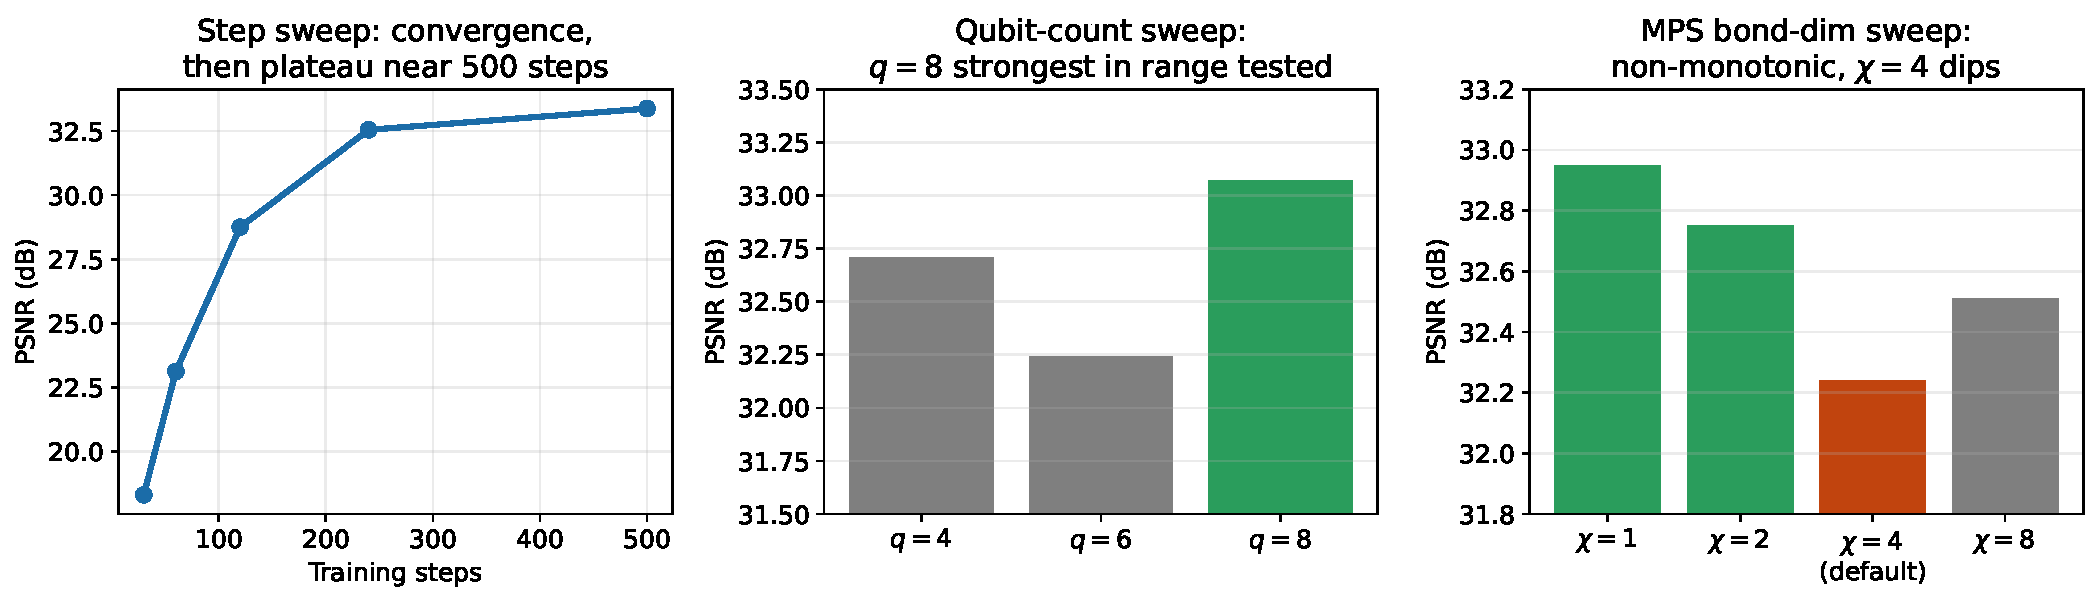
\includegraphics[width=\linewidth]{figures/capacity_scaling_sweeps.pdf}
\caption{Capacity and scaling sweeps from Table~\ref{tab:capacity_ablation} (single-seed, \textit{Monalisa}). Left: PSNR vs.\ training steps, confirming convergence-limited behavior with a plateau near 500 steps. Center: qubit-count sweep, $q=8$ strongest in the tested range. Right: MPS bond-dimension sweep, highlighting the non-monotonic dip at the default $\chi=4$ (orange) relative to both smaller ($\chi=1,2$, green) and larger ($\chi=8$, gray) bond dimensions.}
\label{fig:capacity_scaling_sweeps}
\end{figure}

\begin{table}[H]
\centering
\caption{Capacity and feature-bottleneck sweeps (single-seed; directional, not statistically resolved).}
\label{tab:capacity_ablation}
\scriptsize
\begin{tabular}{lcccc}
\toprule
Experiment & Setting & MSE & PSNR (dB) & SSIM \\
\midrule
Step sweep & 30 steps & $1.4777\times10^{-2}$ & 18.30 & 0.7467 \\
Step sweep & 60 steps & $4.8797\times10^{-3}$ & 23.12 & 0.9306 \\
Step sweep & 120 steps & $1.3336\times10^{-3}$ & 28.75 & 0.9818 \\
Step sweep & 240 steps & $5.5542\times10^{-4}$ & 32.55 & 0.9927 \\
Step sweep & 500 steps & $4.5941\times10^{-4}$ & 33.38 & 0.9938 \\
Qubit count & $q=4$ & $5.3633\times10^{-4}$ & 32.71 & 0.9928 \\
Qubit count & $q=6$ & $5.9771\times10^{-4}$ & 32.24 & 0.9919 \\
Qubit count & $q=8$ & $4.9322\times10^{-4}$ & 33.07 & 0.9933 \\
MPS bond dim. & $\chi=1$ & $5.0746\times10^{-4}$ & 32.95 & 0.9932 \\
MPS bond dim. & $\chi=2$ & $5.3061\times10^{-4}$ & 32.75 & 0.9929 \\
MPS bond dim. & $\chi=4$ & $5.9771\times10^{-4}$ & 32.24 & 0.9919 \\
MPS bond dim. & $\chi=8$ & $5.6124\times10^{-4}$ & 32.51 & 0.9925 \\
No MPS, patch statistics & Patch stats & $5.3874\times10^{-4}$ & 32.69 & 0.9927 \\
\bottomrule
\end{tabular}
\end{table}

\begin{table}[H]
\centering
\caption{Capacity and resource comparison for the held-out CIFAR validation layer. All rows use the same linear readout width and split protocol.}
\label{tab:resource_capacity}
\scriptsize
\begin{tabular}{lcccc}
\toprule
Model & Feature dim. & Readout params. & Pair/CNOT channels & Split \\
\midrule
HVK2D real-CIFAR map & 32 & 2112 & 6 pair / 14 CNOT & 6/4 \\
ZZ-only observables & 32 & 2112 & 3 pair & 6/4 \\
No entanglement & 32 & 2112 & 0 & 6/4 \\
Strict classical random features & 32 & 2112 & 0 & 6/4 \\
Raw/local controls & 32 & 2112 & 0 & 6/4 \\
\bottomrule
\end{tabular}
\end{table}

The same-set CIFAR-10 and \textit{Monalisa} results (Table~\ref{tab:cifar10}) are capacity and positioning diagnostics rather than generalization evidence: HVK2D reaches $34.50$~dB mean PSNR on the five-image native-resolution CIFAR-10 subset, and $40.70$~dB on the $256\times256$ \textit{Monalisa} target, exceeding a 1D control by $5.98$~dB. The high-capacity MLP and CNN baselines remain stronger in pure same-set pixel accuracy (MLP best-case PSNR exceeds $100$~dB, a memorization signature), and neither same-set result should be read against the held-out finding above.

\begin{figure}[H]
\centering
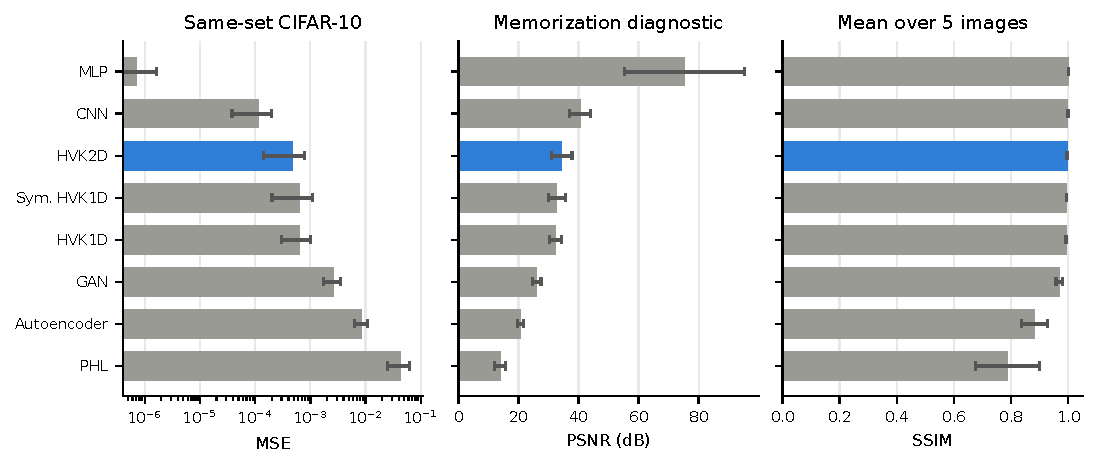
\includegraphics[width=\linewidth]{figures/cifar_metric_comparison.pdf}
\caption{Same-set CIFAR-10 comparison across all eight methods of Table~\ref{tab:cifar10}: MSE (log scale, left), PSNR with the memorization framing made explicit (center), and mean SSIM over the five images (right). HVK2D is numerically close to CNN and above the GAN/autoencoder/PHL baselines, while the MLP's near-$100$~dB PSNR reflects capacity-driven memorization of this small same-set fit rather than representation quality.}
\label{fig:cifar_metric_comparison}
\end{figure}

\begin{table}[H]
\centering
\caption{CIFAR-10 native $32\times32$ same-set reconstruction over five images (not a held-out test).}
\label{tab:cifar10}
\scriptsize
\begin{tabular}{lcccccc}
\toprule
Model & Mean MSE & Best MSE & Mean PSNR & Best PSNR & Mean SSIM & Best SSIM \\
\midrule
MLP & $7.0865\times10^{-7}$ & $7.2702\times10^{-12}$ & 75.14 & 111.38 & 0.99999 & 1.00000 \\
CNN & $1.1648\times10^{-4}$ & $3.3325\times10^{-5}$ & 40.61 & 44.77 & 0.99889 & 0.99928 \\
HVK2D & $4.6655\times10^{-4}$ & $1.3237\times10^{-4}$ & 34.50 & 38.78 & 0.99578 & 0.99743 \\
Symmetric HVK1D & $6.4739\times10^{-4}$ & $2.4391\times10^{-4}$ & 32.81 & 36.13 & 0.99382 & 0.99487 \\
HVK1D & $6.4639\times10^{-4}$ & $3.4381\times10^{-4}$ & 32.42 & 34.64 & 0.99314 & 0.99448 \\
GAN & $2.6448\times10^{-3}$ & $1.4853\times10^{-3}$ & 26.03 & 28.28 & 0.96885 & 0.97665 \\
Classical AE & $8.6021\times10^{-3}$ & $6.3843\times10^{-3}$ & 20.78 & 21.95 & 0.88188 & 0.92745 \\
PHL & $4.3415\times10^{-2}$ & $2.2253\times10^{-2}$ & 14.01 & 16.53 & 0.78792 & 0.91842 \\
\bottomrule
\end{tabular}
\end{table}

\subsection{The Physics-Informed Regularizer's Conditional Value}
Table~\ref{tab:hamiltonian_controls_supp} shows the Hamiltonian energy term is, if anything, a mild drag on reconstruction quality in the present system. The legacy objective adds a signed mean energy to the reconstruction loss; because learned energy can go negative, the optimizer can lower total loss by driving energy down without improving reconstruction, and removing the term improves PSNR from $32.24$ to $33.30$~dB. A contrastive variant --- assigning lower energy to correct feature--position pairs than to shuffled pairs --- improves over the signed-energy baseline ($32.84$~dB) but remains below its own no-energy-loss counterpart ($33.33$~dB). We read this as a case where the reconstruction loss already dominates the optimization signal at this model scale: a physically motivated regularizer has room to help when it resolves an otherwise underdetermined objective, and here the pixel-fidelity loss alone is sufficiently informative that the extra term mostly adds noise to the gradient. This does not mean Hamiltonian regularization is never useful --- only that its value is conditional on the reconstruction loss being under-constrained.

\begin{figure}[H]
\centering
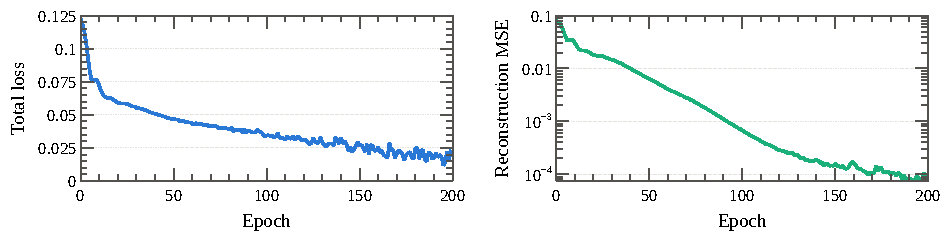
\includegraphics[width=0.95\linewidth]{figures/contrastive_training_curves.pdf}
\caption{Training dynamics for the contrastive Hamiltonian-core run of Table~\ref{tab:hamiltonian_controls_supp}: total loss (left) and reconstruction MSE on a log scale (right) over 200 epochs. Both converge smoothly with no instability introduced by the contrastive energy term.}
\label{fig:contrastive_training_curves}
\end{figure}

\begin{figure}[H]
\centering
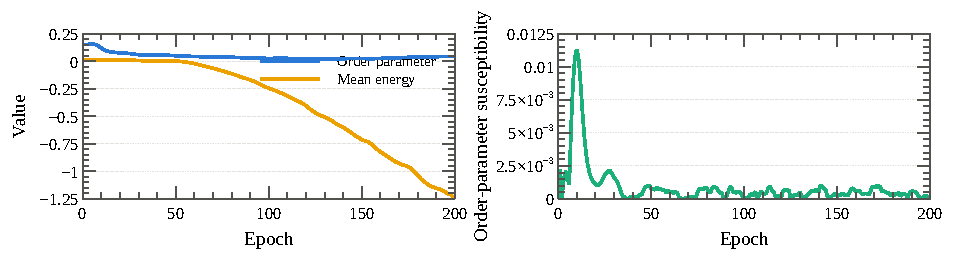
\includegraphics[width=0.95\linewidth]{figures/contrastive_order_parameter_curve.pdf}
\caption{Order parameter and mean Hamiltonian energy (left) and the corresponding one-step order-parameter difference (right) for the same contrastive Hamiltonian-core run. The energy diagnostic drifts steadily negative while the order parameter remains comparatively flat after the initial training period. This is consistent with the energy term being monitored without being the quantity that most improves reconstruction, matching the conditional-value reading of Table~\ref{tab:hamiltonian_controls_supp}.}
\label{fig:contrastive_order_parameter}
\end{figure}

\begin{table}[H]
\centering
\caption{Hamiltonian and observable-sector controls (single-seed). The energy objective is diagnostically useful but does not improve reconstruction accuracy.}
\label{tab:hamiltonian_controls_supp}
\scriptsize
\begin{tabular}{p{0.28\textwidth}cccp{0.25\textwidth}}
\toprule
Experiment & MSE & PSNR (dB) & SSIM & Interpretation \\
\midrule
Legacy baseline, signed energy & $5.9771\times10^{-4}$ & 32.24 & 0.9919 & Standard energy-regularized run \\
No energy loss & $4.6772\times10^{-4}$ & 33.30 & 0.9937 & Removing energy improves PSNR \\
No observable noise & $5.3518\times10^{-4}$ & 32.72 & 0.9928 & Noise is not essential \\
Contrastive Hamiltonian core & $5.1975\times10^{-4}$ & 32.84 & 0.9930 & Stronger objective helps modestly \\
Contrastive, no energy loss & $4.6498\times10^{-4}$ & 33.33 & 0.9937 & Energy removal still performs best \\
ZZ-only observables & $5.1503\times10^{-4}$ & 32.88 & 0.9930 & Nearest-neighbor $ZZ$ largely suffice \\
\bottomrule
\end{tabular}
\end{table}

\subsection{A Reproducibility Note on Table~\ref{tab:hamiltonian_controls_supp}, and an Energy-as-Decoder-Feature Follow-Up}
\label{sec:hamiltonian_followup}
While investigating whether the energy term could be made to actively help reconstruction rather than merely act as a diagnostic (motivated by the conditional-value reading above), we found that Table~\ref{tab:hamiltonian_controls_supp}'s absolute PSNR values are not independently reproducible from the current codebase and documented protocol. Re-running the unmodified legacy-signed-energy, no-energy-loss, and contrastive configurations at the documented protocol (\textit{Monalisa}, $256\times256$/patch=64, \texttt{model\_variant=standard}, 200 steps, seed 42, in an environment matching the paper's stated package versions exactly) reproduces PSNR values 6--12~dB \emph{higher} than published, across every variant tested, not only a new one (Table~\ref{tab:hamiltonian_reproducibility}). The script that generated Table~\ref{tab:hamiltonian_controls_supp}'s original numbers is referenced only in commit messages and was never actually committed to the repository (the referenced path lies inside a gitignored directory, and \texttt{git cat-file} confirms no corresponding blob exists in any commit), so the original protocol could not be recovered to explain the gap directly; a shorter-step rerun ruled out step count alone as the explanation. Rather than block on an unrecoverable protocol, we adopt this fresh, same-environment reproduction as the baseline for the remainder of this section, disclosing the gap here explicitly rather than silently revising Table~\ref{tab:hamiltonian_controls_supp}'s historical values. The qualitative finding is unchanged under the new environment: removing the energy loss still improves PSNR (here $38.63\rightarrow44.56$~dB) exactly as it does in Table~\ref{tab:hamiltonian_controls_supp} ($32.24\rightarrow33.30$~dB) --- only the absolute PSNR scale differs between the two protocols, not the sign or approximate size of the effect. We also reran the remaining two observable-sector rows from Table~\ref{tab:hamiltonian_controls_supp} (no observable noise, ZZ-only) at the identical protocol; unlike the three variants above, these land within $1$~dB of the published values ($32.75$ vs.\ $32.72$~dB, and $32.11$ vs.\ $32.88$~dB, respectively) rather than 6--12~dB higher. We do not have a confirmed explanation for why these two rows reproduce so much more closely than the other three under the same rerun protocol; we report the observation plainly rather than speculate.

\begin{table}[H]
\centering
\caption{Fresh, same-environment reproduction of Table~\ref{tab:hamiltonian_controls_supp}'s configurations (\textit{Monalisa}, 200 steps, seed 42), alongside two new coupling/objective variants. Absolute PSNR is not directly comparable to Table~\ref{tab:hamiltonian_controls_supp} for the first three rows (see reproducibility note above); the two observable-sector rows are close to their Table~\ref{tab:hamiltonian_controls_supp} counterparts.}
\label{tab:hamiltonian_reproducibility}
\scriptsize
\begin{tabular}{lcc}
\toprule
Config & PSNR (dB) & Note \\
\midrule
Legacy signed energy (linear, unbounded coupling) & 38.63 & Table~\ref{tab:hamiltonian_controls_supp}'s legacy baseline, rerun \\
No energy loss & 44.56 & Table~\ref{tab:hamiltonian_controls_supp}'s no-energy-loss control, rerun \\
Contrastive energy, unbounded coupling & 42.92 & Table~\ref{tab:hamiltonian_controls_supp}'s contrastive variant, rerun \\
No observable noise & 32.75 & Table~\ref{tab:hamiltonian_controls_supp}'s no-noise control, rerun; within $0.03$~dB of published \\
ZZ-only observables & 32.11 & Table~\ref{tab:hamiltonian_controls_supp}'s ZZ-only control, rerun; within $0.77$~dB of published \\
Positive/squared energy, unbounded coupling & 44.69 & Untested in the original Table~\ref{tab:hamiltonian_controls_supp} \\
Bounded coupling ($\tanh$) + positive energy & 44.56 & Root-cause fix for the unbounded-coupling pathology (see text) \\
Bounded coupling + contrastive energy & 43.01 & \\
\bottomrule
\end{tabular}
\end{table}

The root cause of the legacy objective's drag, beyond what Table~\ref{tab:hamiltonian_controls_supp} alone shows: the learned couplings $J_x,J_y,J_z$ feed only the energy loss and never reach the decoder, so under a linear (signed) energy loss the optimizer can drive them to unbounded magnitude to cheaply lower total loss with no reconstruction benefit, competing with the reconstruction gradient on shared circuit weights. Bounding the couplings ($\tanh$) and switching to the already-implemented but previously untested \texttt{positive} (squared) energy-loss mode removes this pathology --- bounded-coupling + positive energy \emph{ties} the no-energy-loss control ($44.56$ vs.\ $44.56$--$44.69$~dB at seed 42) rather than beating it: the fix stops the Hamiltonian term from actively \emph{hurting} reconstruction, but by construction it still cannot \emph{help}, since energy never reaches the decoder.

To let the energy signal actually help reconstruction rather than only avoid hurting it, we additionally feed the learned energy into the decoder as an input feature, concatenated alongside observables and positions, rather than using it only as a side-channel loss term. Table~\ref{tab:hamiltonian_decoder_feature} gives the full 3-seed result against the no-energy-loss baseline. Two of three seeds show a real improvement (up to $+1.25$~dB); the third shows a $-5.08$~dB regression that outweighs both wins combined, so the mean delta across seeds is negative ($\approx-1.1$~dB). We read this as a genuinely different and weaker claim than ``the Hamiltonian term now helps'': feeding energy into the decoder increases outcome variance more than it reliably improves the mean, and is better characterized as a promising but seed-sensitive direction than a validated fix. A larger multi-seed study (5+ seeds) would be needed before claiming either that this construction reliably helps or that it is neutral; until then, the conservative framing above --- energy as an interpretability/diagnostic signal rather than a performance-improving inductive bias --- remains the safer default characterization for the main text.

\begin{table}[H]
\centering
\caption{Feeding the learned Hamiltonian energy into the decoder as an input feature, vs.\ the no-energy-loss baseline (\textit{Monalisa}, 200 steps, 3 seeds). Not a robust win: two of three seeds improve, one regresses sharply enough that the mean delta across seeds is negative ($\approx-1.1$~dB).}
\label{tab:hamiltonian_decoder_feature}
\scriptsize
\begin{tabular}{lccc}
\toprule
Seed & No energy loss (dB) & Energy fed to decoder (dB) & $\Delta$ (dB) \\
\midrule
42 & 44.56 & 45.81 & $+1.25$ \\
43 & 43.77 & 44.28 & $+0.51$ \\
44 & 45.33 & 40.25 & $-5.08$ \\
\bottomrule
\end{tabular}
\end{table}

\subsection{Restricted Diagnostic and Training-Trace Provenance Audit}
\label{sec:restricted_ablation}
The main paper's restricted pair-correlation result remains supported by the five-seed final metrics: the entangling observable map reaches mean $R^2=0.9735$, versus $R^2\leq0.02$ for the tested non-entangling controls. Figure~\ref{fig:restricted_diagnostic_summary} displays those measured final metrics.

\begin{figure}[H]
\centering
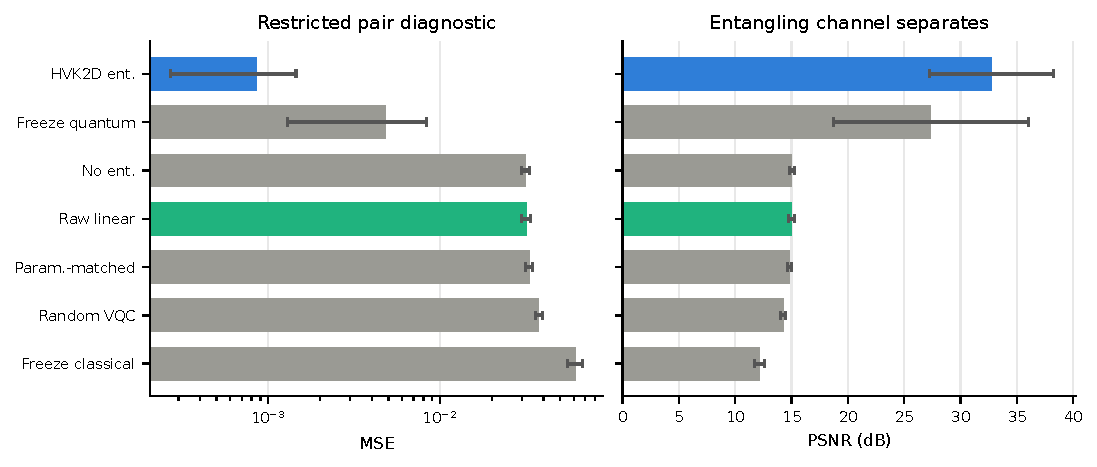
\includegraphics[width=\linewidth]{figures/full_ablation_metric_comparison.pdf}
\caption{The restricted pair-correlation diagnostic underlying the entanglement-necessity result (mean $R^2=0.9735$ vs.\ $R^2\leq0.02$ for non-entangling controls), shown here as MSE (left) and PSNR (right) across the full variant set: the trained HVK2D entangling map, freeze-quantum, no-entanglement, raw-linear, parameter-matched classical, random-VQC, and freeze-classical. The entangling channel (blue) separates numerically from every non-entangling control on this target, in direct contrast to the ordinary held-out reconstruction result of Section~\ref{sec:holdout_headline} where the same entangling channel does not separate from local/raw controls --- the two figures together visualize this document's central task-dependence argument.}
\label{fig:restricted_diagnostic_summary}
\end{figure}

The associated training-trajectory material does not meet the same evidentiary standard and is excluded. The per-variant curves previously produced by \path{run_newhvk_suite.py::epoch_tables} are analytic interpolations from final metrics, not logged epoch measurements. Separately, the 13 stored real-image traces were recorded from HVK2D in training mode, whose forward pass adds Gaussian noise with standard deviation $0.01$ to every observable; their maximum one-step changes therefore mix optimizer dynamics with injected jitter. Neither source supports a training-reorganization comparison. The corrected multi-dataset runner now records a noise-free evaluation-mode forward pass after each optimizer update and preserves aggregate summaries across partial runs. A fresh multi-seed execution is required before training-dynamics claims or figures are restored.

\section{HVK1D versus HVK2D: A Direct Topology Comparison}
\label{sec:topology_comparison}
The main paper introduces both the HVK1D (6-qubit chain) and HVK2D ($2\times3$ grid) topologies, but until now the only direct comparison was the same-set CIFAR-10 fit of Table~\ref{tab:cifar10}. Here we compare the two topologies directly under matched conditions --- identical qubit count (6, native to both), identical feature width, identical decoder architecture and step budget --- on held-out generalization rather than same-set fitting, on two evidence bases: a fast analytic-surrogate sweep at full statistical scope, and a smaller real-trained-circuit confirmation subset. The two topologies are close in parameter count by construction (HVK1D: 53{,}787; HVK2D: 52{,}755) but not identical, since their circuit structures differ (chain vs. grid connectivity, 27 vs. 19 measured observables); we report this honestly rather than forcing an artificial match.

\subsection{Real-Circuit Confirmation}
\label{sec:topology_real_circuit}
Each topology was trained jointly on 2 CIFAR-10 images (native $32\times32$, overlapping $8\times8$ patches at stride 4, 49 patches/image --- the same convention as Table~\ref{tab:cifar10}) for a reduced 90-step budget across 3 seeds, then evaluated by direct forward pass (no retraining) on 3 further CIFAR-10 images from different classes never seen in training (airplane, frog, automobile) --- a genuine held-out test. The reduced step budget and seed count follow directly from a measured timing calibration on this project's GPU (NVIDIA GTX 1050): at the full 200-step budget used elsewhere in this document, the complete topology comparison at the scope below would cost single-digit hours rather than the tens of minutes actually spent; we report this budget explicitly rather than silently shrinking scope.

\begin{table}[H]
\centering
\caption{Real-trained-circuit topology comparison: held-out reconstruction on 3 unseen CIFAR-10 images (9 image-seed pairs per topology: 3 seeds $\times$ 3 held-out images), 90-step budget.}
\label{tab:topology_real_circuit}
\scriptsize
\begin{tabular}{lcccc}
\toprule
Topology & Params & Held-out PSNR (dB) & Held-out SSIM & Wall time / run (min) \\
\midrule
HVK1D & 53{,}787 & $11.73\pm1.99$ & $0.317\pm0.227$ & $29.6\pm9.0$ \\
HVK2D & 52{,}755 & $11.57\pm1.53$ & $0.304\pm0.188$ & $16.6\pm0.3$ \\
\bottomrule
\end{tabular}
\end{table}

The two topologies give close held-out reconstruction means at this scale. Across the 9 image--seed pairs, the paired HVK1D-minus-HVK2D difference is $0.16$~dB. After aggregating the three image differences within each seed, the seed-bootstrap 95\% CI is $[-0.38,0.46]$~dB and the two-sided Wilcoxon test gives $p=0.50$. The 3-seed, 3-image subset is too small to establish formal equivalence. HVK2D nevertheless completes the same 90-step budget in roughly half the wall-clock time of HVK1D at a comparable parameter count, a measured resource-cost difference. This is consistent with HVK2D's smaller measured observable set (19 vs.\ 27); the corresponding transpiled depth and two-qubit-gate counts are shown in Figure~\ref{fig:ibm_circuit_summary}. At the tested scale, the evidence supports treating topology primarily as a resource-cost choice rather than claiming an accuracy difference.

\subsection{Surrogate Sweep: Full Statistical Scope}
\label{sec:topology_surrogate}
To reach the seed and dataset breadth a held-out comparison needs, we extend the existing analytic-surrogate held-out framework (already used for Tables~\ref{tab:hvk_real_cifar}--\ref{tab:multi_dataset_classification}) with an HVK1D-equivalent feature map. The existing HVK2D surrogate (\texttt{real\_newhvk\_features}) is a closed-form proxy built from six index-pairs of the local-observable block, standing in for the grid circuit's pairwise $ZZ$ correlators. The new HVK1D surrogate is not a relabeled copy: it iterates the chain topology's actual five nearest-neighbor bonds (vs.\ the grid's seven-edge pattern) and adds a second, distinct pair-type term reflecting HVK1D's extra $XX$/$YY$ measurement channels that the 2D grid circuit does not have (it measures only $Z$, $X$, $ZZ$). Both surrogates share the same local/positional input convention, so the comparison is apples-to-apples. We run the full held-out reconstruction and downstream-classification battery (5 seeds, stratified splits) across CIFAR-10, Fashion-MNIST, and PathMNIST.

\begin{table}[H]
\centering
\caption{Surrogate-sweep topology comparison (5 seeds, held-out reconstruction PSNR and downstream classification accuracy), against the strongest classical control (raw-linear) for reference.}
\label{tab:topology_surrogate}
\scriptsize
\begin{tabular}{lccc}
\toprule
Dataset / metric & HVK1D-pair & HVK2D-pair & raw-linear \\
\midrule
CIFAR-10, PSNR (dB) & $19.21\pm2.22$ & $19.28\pm2.25$ & $20.48\pm2.32$ \\
CIFAR-10, accuracy & $0.240\pm0.102$ & $0.260\pm0.102$ & $0.240\pm0.102$ \\
Fashion-MNIST, PSNR (dB) & $17.22\pm1.68$ & $17.24\pm1.69$ & $17.56\pm1.65$ \\
Fashion-MNIST, accuracy & $0.574\pm0.021$ & $0.578\pm0.015$ & $0.654\pm0.020$ \\
PathMNIST, PSNR (dB) & $26.07\pm5.36$ & $26.07\pm5.33$ & $26.60\pm5.57$ \\
PathMNIST, accuracy & $0.560\pm0.046$ & $0.558\pm0.041$ & $0.596\pm0.041$ \\
\bottomrule
\end{tabular}
\end{table}

\begin{figure*}[t]
\centering
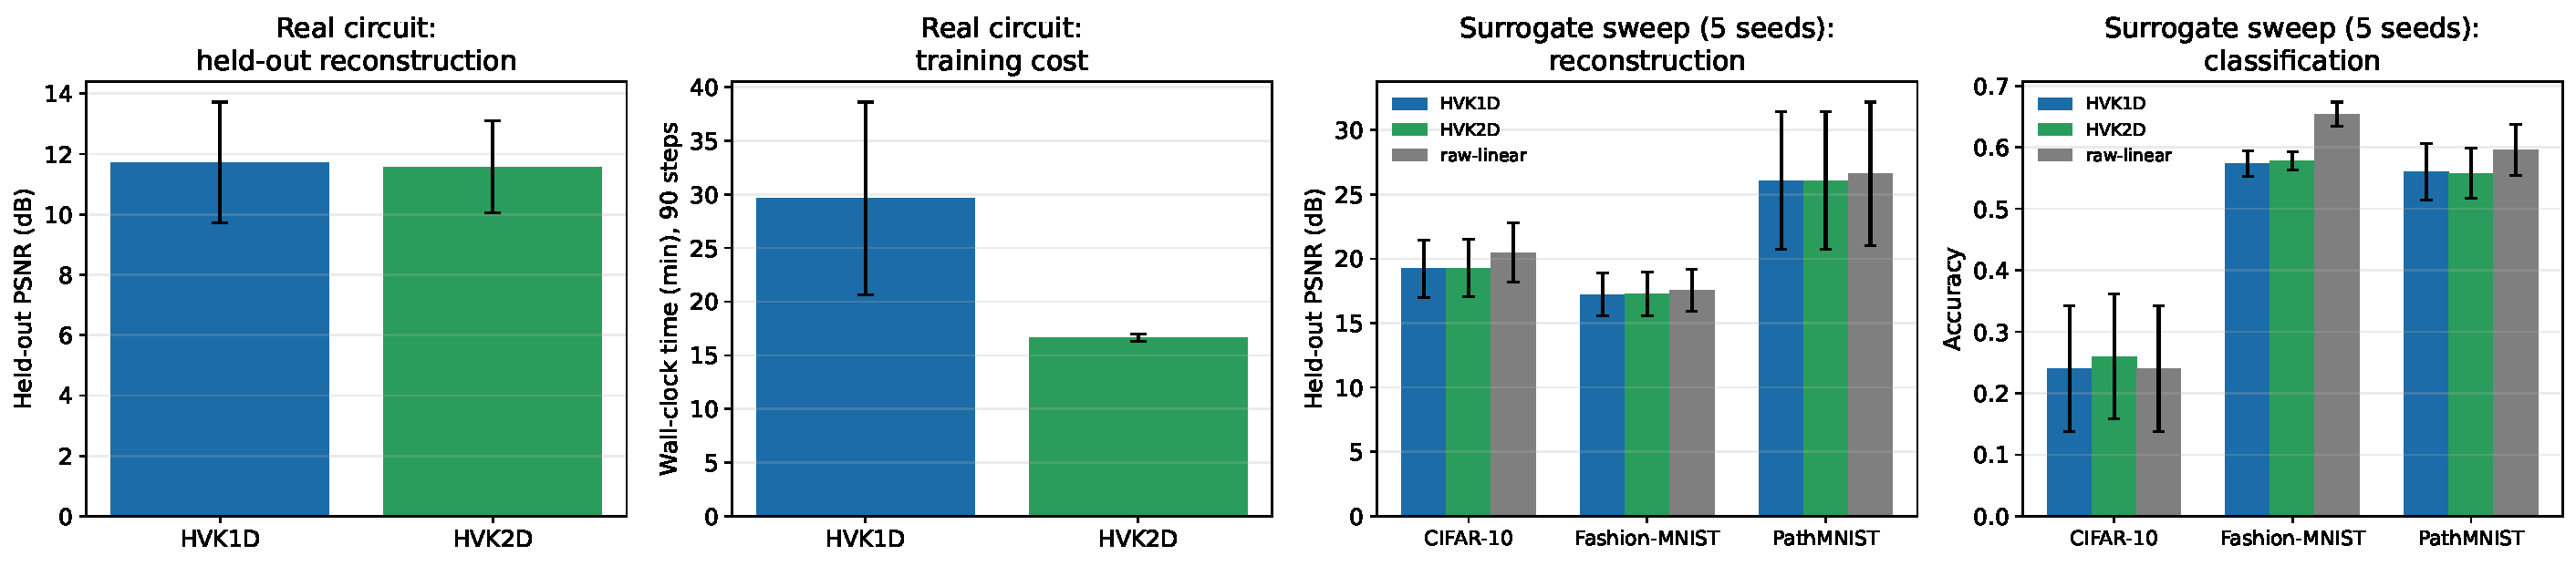
\includegraphics[width=0.95\textwidth]{figures/topology_comparison_summary.pdf}
\caption{HVK1D vs.\ HVK2D across both evidence bases. Left two panels: real-circuit held-out PSNR and per-run wall-clock time (90-step budget, 3 seeds, error bars = std). Right two panels: surrogate-sweep held-out reconstruction PSNR and classification accuracy across three datasets (5 seeds), both topologies plotted against the strongest classical control (raw-linear).}
\label{fig:topology_comparison_summary}
\end{figure*}

The broader surrogate sweep reproduces the real-circuit pattern: HVK1D-pair and HVK2D-pair track each other closely on every dataset and metric (PSNR differs by at most $0.07$~dB, accuracy by at most $2$ percentage points), and both sit slightly below the raw-linear control. For inference, held-out image differences are first averaged within each split seed so that images sharing a fitted readout are not treated as independent replicates. The seed-level HVK1D-minus-HVK2D PSNR differences are $-0.070$~dB on CIFAR-10 (bootstrap 95\% CI $[-0.151,0.024]$, Wilcoxon $p=0.3125$), $-0.021$~dB on Fashion-MNIST (CI $[-0.033,-0.006]$, $p=0.125$), and $0.003$~dB on PathMNIST (CI $[-0.012,0.015]$, $p=0.625$), all at $n=5$ seeds. The Fashion-MNIST percentile interval excludes zero, but the discrete seed-level signed-rank test does not resolve the difference; we therefore describe it as numerically small rather than statistically established. Neither topology shows a general reconstruction/classification advantage over simple classical baselines, and the evidence supports treating topology as a resource-cost choice at the tested scale. Section~\ref{sec:restricted_ablation}'s restricted, leakage-audited diagnostic remains the setting where entanglement structure matters within the tested feature/readout class.

\section{Held-Out Output-Level \texorpdfstring{$D_4$}{D4} Symmetry Evaluation}
\label{sec:d4_symmetry_experiment}
The main paper's $D_4$-equivariance claim (pooled HVK2D observable map, equivariance error $9.57\times10^{-17}$) was previously demonstrated at feature-grid level on 1,000 cached CIFAR-10 images, giving 7,000 image--nonidentity-transform evaluations. That large numerical check did not use a fitted readout, a held-out reconstruction protocol, or a classical baseline sharing the same pooling construction, and therefore did not measure what equivariance costs or buys at the output level. This section closes those gaps with a held-out, multi-seed (5 seeds, 20 train / 10 held-out images per seed, disjoint CIFAR-10 splits) experiment across five modes: the provably-equivariant \emph{D4-pooled-HVK2D} map; a new \emph{D4-pooled-classical} baseline applying the identical Reynolds-averaging construction (group-averaging the feature map over the eight $D_4$ transforms) to the purely classical \emph{local-raw} feature map instead of the HVK2D-surrogate one, so the comparison is architecture-matched rather than quantum-vs-nothing; the non-symmetric \emph{HVK2D-positional} control; an \emph{ordinary-augmentation} baseline (\emph{HVK2D-augmented}: the same non-pooled feature map, but with a ridge readout trained on all eight $D_4$-transformed copies of every training image, instead of architectural pooling); and the non-symmetric classical \emph{local-raw} control. For every mode we measure both \emph{feature-equivariance error} (as before) and, new here, \emph{output consistency}: for each held-out image we predict a reconstruction from every one of its 8 $D_4$-transformed copies, rotate/reflect each prediction back to canonical orientation, and measure the pairwise mean-squared disagreement between the 8 canonicalized predictions, together with reconstruction accuracy (PSNR) against ground truth.

\begin{table}[H]
\centering
\caption{Held-out output-level $D_4$ symmetry evaluation (5 seeds, 10 held-out images/seed). Feature-equivariance error and output-consistency MSE are reported at $\pm$std over seeds; both span many orders of magnitude between pooled and non-pooled modes.}
\label{tab:d4_symmetry_experiment}
\scriptsize
\begin{tabular}{lccc}
\toprule
Mode & Equivariance error & Output consistency (MSE) & Accuracy PSNR (dB) \\
\midrule
D4-pooled (HVK2D) & $(9.47\pm0.25)\times10^{-17}$ & $(3.19\pm1.66)\times10^{-21}$ & $14.97\pm0.53$ \\
D4-pooled (classical) & $(8.94\pm0.22)\times10^{-17}$ & $(1.37\pm0.96)\times10^{-23}$ & $15.12\pm0.52$ \\
HVK2D (non-symmetric) & $0.8163\pm0.0070$ & $0.01149\pm0.00213$ & $15.12\pm0.59$ \\
HVK2D (ordinary aug.) & $0.8163\pm0.0070$ & $0.01055\pm0.00226$ & $15.30\pm0.56$ \\
local-raw (classical) & $0.8380\pm0.0067$ & $0.01202\pm0.00245$ & $15.16\pm0.68$ \\
\bottomrule
\end{tabular}
\end{table}

\begin{figure*}[t]
\centering
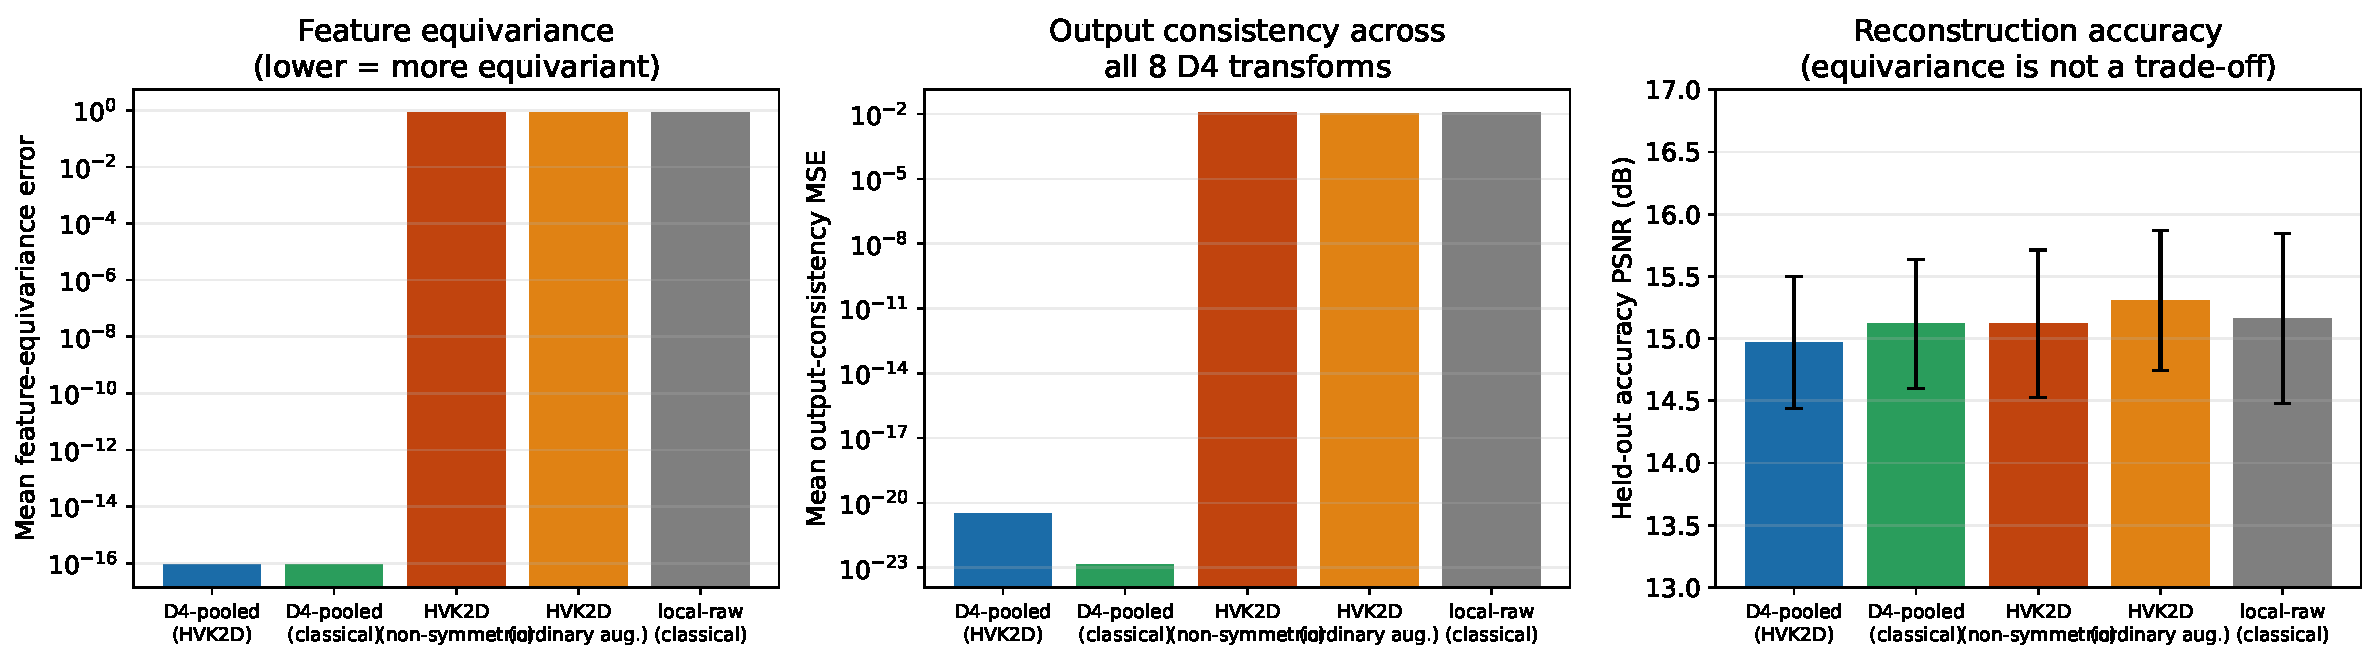
\includegraphics[width=0.95\textwidth]{figures/d4_symmetry_experiment_summary.pdf}
\caption{Held-out output-level $D_4$ symmetry evaluation, 5 seeds. Left: feature-equivariance error (log scale) --- both pooled modes sit at floating-point precision, roughly 16 orders of magnitude below every non-pooled control. Center: output-consistency MSE across all 8 $D_4$ transforms (log scale) --- the same separation persists at the reconstruction-output level, not just the feature level. Right: held-out accuracy PSNR (linear scale, error bars = std) --- the five mean values are close relative to their between-seed variation; no formal equivalence claim is made.}
\label{fig:d4_symmetry_experiment_summary}
\end{figure*}

Four findings follow. First, the Reynolds-averaging construction that gives HVK2D its provable equivariance is not specific to the quantum-surrogate feature map: applying the identical pooling operation to a purely classical local-observable map produces the same floating-point-precision equivariance ($8.94\times10^{-17}$ vs.\ $9.47\times10^{-17}$), confirming the guarantee is a property of the group-averaging construction itself, not of anything intrinsically quantum. Second, the separation between pooled and non-pooled modes is not an artifact of measuring features in isolation: it persists essentially unchanged at reconstruction output (output-consistency MSE $\sim10^{-21}$--$10^{-23}$ for pooled modes vs.\ $\sim0.010$--$0.012$ for non-pooled controls). Third, ordinary augmentation cannot change feature-equivariance error, but it reduces output-consistency MSE by roughly $8\%$ ($0.01055$ vs.\ $0.01149$). Fourth, exact pooling has a small accuracy trade-off relative to ordinary augmentation: pooled HVK2D is lower by $0.336$~dB on average across the five paired seeds (seed-bootstrap 95\% CI $[-0.441,-0.231]$~dB; two-sided Wilcoxon $p=0.0625$, the smallest attainable nonzero two-sided value at $n=5$). The symmetry guarantee is decisive, while the available sample supports a modest rather than zero accuracy cost.

\subsection{Real-Circuit Confirmation}
\label{sec:d4_real_circuit}
Everything above is measured on the closed-form analytic surrogate. This subsection repeats the pooled-vs-non-pooled equivariance and output-consistency comparison on the \emph{actual trained quantum circuit} --- the same four already-trained HVK2D checkpoints used for the main paper's real IBM-hardware pilot (\textit{cat}, \textit{ship/hydrofoil}, \textit{ship/sea boat}, \textit{airplane}), replayed with no retraining. For each image we run the trained model's real PennyLane forward pass (exact statevector simulation of the trained weights, not the surrogate formula) on all eight $D_4$-transformed copies of the full image, and compute the same feature-equivariance error and output-consistency MSE as above, both without pooling and with the identical Reynolds-averaging construction applied to the real circuit's own output grid.

\begin{table}[H]
\centering
\caption{Real-trained-circuit $D_4$ confirmation: exact PennyLane forward pass on four already-trained HVK2D hardware-pilot checkpoints, no retraining.}
\label{tab:d4_real_circuit}
\scriptsize
\begin{tabular}{lccc}
\toprule
Image & Mode & Equivariance error & Output consistency (MSE) \\
\midrule
cat & non-pooled & $0.0760$ & $0.01869$ \\
cat & D4-pooled & $5.50\times10^{-8}$ & $9.78\times10^{-16}$ \\
ship (hydrofoil) & non-pooled & $0.3905$ & $0.06437$ \\
ship (hydrofoil) & D4-pooled & $5.25\times10^{-8}$ & $1.83\times10^{-15}$ \\
ship (sea boat) & non-pooled & $0.4054$ & $0.05451$ \\
ship (sea boat) & D4-pooled & $5.65\times10^{-8}$ & $1.24\times10^{-15}$ \\
airplane & non-pooled & $0.2387$ & $0.03662$ \\
airplane & D4-pooled & $5.16\times10^{-8}$ & $1.80\times10^{-15}$ \\
\midrule
Mean & non-pooled & $0.2777$ & $0.04355$ \\
Mean & D4-pooled & $5.39\times10^{-8}$ & $1.46\times10^{-15}$ \\
\bottomrule
\end{tabular}
\end{table}

The real-circuit result confirms the surrogate's finding directly: pooling collapses the equivariance error from $\mathcal{O}(10^{-1})$ to $\mathcal{O}(10^{-8})$ and output-consistency MSE from $\mathcal{O}(10^{-2})$ to $\mathcal{O}(10^{-15})$, an 8--13 order-of-magnitude gap on every one of the four images, with no exceptions. The pooled real circuit's residual error ($\sim\!5\times10^{-8}$) is larger than the surrogate's floating-point-precision result ($\sim\!10^{-17}$) because the real circuit involves a full statevector simulation of the trained gates plus a fresh per-transform feature-standardization step, both of which accumulate ordinary floating-point noise that the closed-form surrogate formula does not --- the pooled result is exact up to numerical precision, not exact to the same sixteen digits as a symbolic identity, which is the expected and unremarkable difference between an analytic proxy and an actual simulated circuit.

\section{Exact Circuit and Hamiltonian Definitions}
\label{sec:supp_exact_circuits}
For a one-dimensional chain of $n_{\text{bonds}}$ bonds indexed by $i$ and sites $(i,i+1)$, the anisotropic Heisenberg Hamiltonian is
\begin{align}
H_{\text{Heis}}=\sum_{i=0}^{n_{\text{bonds}}-1}\Bigl(
J_x^{(i)}X_iX_{i+1}+J_y^{(i)}Y_iY_{i+1}\nonumber\\
{}+J_z^{(i)}Z_iZ_{i+1}\Bigr).
\end{align}
Here $X,Y,Z$ are Pauli operators and $J_\alpha^{(i)}$ are bond-resolved couplings. HVK1D fixes six sites and treats the 15 coefficients on its five bonds as learnable parameters initialized independently from a zero-mean Gaussian with standard deviation $0.1$. Given patch $n$'s measured observables, its energy diagnostic is
\begin{equation}
\mathcal{E}_n(\theta,J) = \sum_{i=0}^{4}\sum_{\alpha\in\{x,y,z\}} J_\alpha^{(i)}\langle\sigma_\alpha^{(i)}\sigma_\alpha^{(i+1)}\rangle_n.
\end{equation}
HVK2D instead uses the seven edges $\mathcal{G}_{2D}$ of its $2\times3$ circuit graph and the implemented grid-Ising diagnostic $\mathcal{E}^{2D}_n=\sum_{(u,v)\in\mathcal{G}_{2D}}j_{uv}\langle Z_uZ_v\rangle_n$. Thus ``Hamiltonian diagnostic'' refers to the full $XX/YY/ZZ$ chain energy for HVK1D and the learned $ZZ$ graph energy for HVK2D. In either case, the patch-averaged term is $\mathcal{L}_{\text{energy}}=\frac{1}{N}\sum_n \mathcal{E}_n$, and the total objective is
\begin{align}
\mathcal{L}_{\text{total}}&=\mathcal{L}_{\text{rec}}
+\lambda\,\mathcal{L}_{\text{energy}},\\
\mathcal{L}_{\text{rec}}&=\frac{1}{N}\sum_{n=1}^{N}
\bigl\|D(o_n,e_n)-P_n\bigr\|_F^2.
\end{align}
with $D$ the classical decoder and $P_n$ the ground-truth patch.

\begin{sloppypar}
Per-patch coordinates $(r_i,c_j)$ are mapped to Fourier features $e_{4k}=\sin(\omega_k\pi r_i)$, $e_{4k+1}=\cos(\omega_k\pi r_i)$, $e_{4k+2}=\sin(\omega_k\pi c_j)$, and $e_{4k+3}=\cos(\omega_k\pi c_j)$ \cite{Xu2021}. HVK1D uses $k\in\{0,1\}$ (8-D), whereas the native-resolution HVK2D implementation uses one frequency (4-D); a learned linear map projects either vector to six $R_Y$ angles. Both six-qubit circuits first apply $U_{\text{enc}}(x_n)=\bigotimes_{i=0}^{5}R_X(x_n^{(i)})$ and $U_{\text{pos}}=\bigotimes_{i=0}^{5}R_Y(\theta_{\text{position}}^{(i)})$. Each of two HVK1D layers then applies per-qubit $\mathrm{Rot}$ gates followed by the strongly-entangling CNOT ring. Each HVK2D layer applies CNOTs over the four horizontal and three vertical grid edges followed by per-qubit $\mathrm{Rot}$ gates, matching the executed source and hardware-replay circuits.

HVK1D returns local $Z/X$ measurements and the three nearest-neighbor pair sectors $ZZ/XX/YY$ (27 values); HVK2D returns local $Z/X$ measurements and grid-edge $ZZ$ correlations (19 values). Positional rotations and fixed graph connectivity distinguish circuit sites, so neither unpooled map is asserted to be permutation- or $D_4$-equivariant. The $D_4$ action in the main paper is instead the explicit permutation action on the $4\times4$ patch grid, and equivariance follows only after the stated Reynolds average over its eight transformations.
\end{sloppypar}

\section{Hardware Pilot Methodology}
\label{sec:hardware_methodology}
The main paper reports a real IBM Quantum hardware reconstruction pilot (five images: \textit{Monalisa} and four CIFAR-10 images, each optimized per-image, hardware PSNR $25.90$--$31.52$~dB against $36.56$--$46.79$~dB in noiseless simulation). This section gives the complete methodology.

\subsection{Reused Checkpoints}
No model was retrained for this pilot. Two pre-existing artifacts were reused directly. The first was the ``shared VQC baseline'' Monalisa checkpoint under
\begin{quote}
\small\path{main2/newHVK/results/ablation_study/legacy_hvk_controls/eval_controls/}\newline\path{shared-baseline-seed-42/}.
\end{quote}
This is the run underlying the ``Legacy baseline, signed energy'' row of Table~\ref{tab:hamiltonian_controls_supp} ($32.24$~dB simulator PSNR). The second set comprised four fresh HVK2D checkpoints trained for 200 steps with Adam ($\eta=0.004$) on an NVIDIA GTX~1050. Each checkpoint corresponds to one native-resolution $32\times32$ CIFAR-10 image optimized directly on its own target, following the same per-image protocol as \textit{Monalisa} rather than the held-out suite of Section~\ref{sec:holdout_headline}. Non-overlapping $8\times8$ patches give 16 patches per image, matching the Monalisa pilot's patch count and keeping the hardware circuit budget predictable.

\subsection{Circuit Reconstruction}
The trained HVK1D forward pass applies, per patch: $R_X$ angle embedding, $R_Y$ positional modulation, then two \texttt{StronglyEntanglingLayers} (per-wire $R_Z$-$R_Y$-$R_Z$ rotations with a CNOT ring whose range increments by layer). We rebuilt this gate-for-gate in Qiskit. Because the trained circuit measures $Z$, $X$, $ZZ$, $XX$, and $YY$ (27 observables), and pairwise correlators are recoverable as joint parities of the \emph{same} all-$Z$/all-$X$/all-$Y$ basis measurements that already give the single-qubit marginals, only three measurement circuits per patch are needed. For 16 Monalisa patches this is $16\times3=48$ circuits. The HVK2D grid circuit is simpler (two layers of fixed grid-edge CNOTs then per-qubit rotations) and measures only $Z$, $X$, $ZZ$ (19 observables, no $XX$/$YY$), so only two measurement circuits per patch are needed: for four CIFAR images at 16 patches each, $4\times16\times2=128$ circuits.

\begin{figure}[H]
\centering
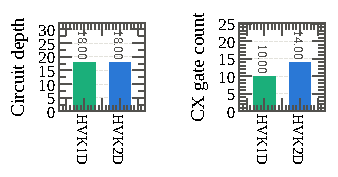
\includegraphics[width=0.75\linewidth]{figures/ibm_circuit_summary.pdf}
\caption{Transpiled circuit resource comparison between the HVK1D (\textit{Monalisa}) and HVK2D (CIFAR) per-patch circuits at \texttt{optimization\_level=1} on \texttt{ibm\_fez}: circuit depth (left) and CX-gate count (right). Both circuits have depth 18 and use 10--14 CX gates. These resource counts document the executed circuits; they do not by themselves attribute the observed hardware--simulator PSNR gap to a particular noise source.}
\label{fig:ibm_circuit_summary}
\end{figure}

\subsection{Local Validation Before Any Hardware Submission}
Every circuit was validated against the cached, training-time observable vectors via an exact Qiskit statevector simulation, \emph{before} any job was submitted to real hardware.

\begin{table}[H]
\centering
\caption{Local validation: Qiskit statevector reconstruction vs.\ cached PennyLane training-time observables.}
\begin{tabular}{lcc}
\toprule
Checkpoint & Patches validated & Max abs.\ error \\
\midrule
Monalisa (HVK1D) & 16 & $7.89\times10^{-4}$ \\
CIFAR cat (HVK2D) & 16 & $9.42\times10^{-6}$ \\
CIFAR ship, hydrofoil (HVK2D) & 16 & $7.76\times10^{-6}$ \\
CIFAR ship, sea boat (HVK2D) & 16 & $7.89\times10^{-6}$ \\
CIFAR airplane (HVK2D) & 16 & $7.14\times10^{-6}$ \\
\bottomrule
\end{tabular}
\end{table}

All translation discrepancies are small relative to the observable perturbations induced by finite-shot device execution: across the five checkpoints, the hardware--statevector mean absolute observable deviation is $0.096$--$0.125$ (maximum $0.218$--$0.340$), versus a maximum translation discrepancy of $7.89\times10^{-4}$ for Monalisa and $9.42\times10^{-6}$ for CIFAR. They therefore rule out a gate-translation mismatch of the measured magnitude as the primary explanation for the hardware--simulator PSNR gap. This pilot does not separate sampling noise, gate/readout errors, drift, and transpilation effects.

\subsection{IBM Quantum Account, Backend, and Job Identifiers}
Jobs were submitted via \texttt{qiskit-ibm-runtime} (channel \texttt{ibm\_quantum\_platform}) under a free/open-plan instance. Both pilots ran on \texttt{ibm\_fez}, a 156-qubit Heron-class processor. Transpilation used \texttt{optimization\_level=1}; each job used \texttt{SamplerV2} with 256 shots per circuit.

\begin{table}[H]
\centering
\caption{IBM Quantum job identifiers (backend: \texttt{ibm\_fez}, 256 shots/circuit).}
\scriptsize
\begin{tabular}{llcc}
\toprule
Image & Job ID & Circuits & Bases \\
\midrule
Monalisa & \texttt{d9ecu34inv1c73aq3qt0} & 48 & Z, X, Y \\
CIFAR cat & \texttt{d9edfo2neu4c739ob2ig} & 32 & Z, X \\
CIFAR ship (hydrofoil) & \texttt{d9edg5cjeosc73filhng} & 32 & Z, X \\
CIFAR ship (sea boat) & \texttt{d9edgakjeosc73filhug} & 32 & Z, X \\
CIFAR airplane & \texttt{d9edgdphtsac739e4kdg} & 32 & Z, X \\
\bottomrule
\end{tabular}
\end{table}

Total: 176 circuits across 5 jobs. Quota consumption, read from \texttt{QiskitRuntimeService.}\allowbreak\texttt{usage()} immediately before and after the pilot, changed from $19$ to $35$ seconds against a $600$-second monthly free-plan allowance. Thus the account meter indicated 16 seconds of billed quantum-processor time and 565 seconds remaining afterward, at an observed rate of $\approx\!0.09$--$0.13$~s/circuit. The readings were recorded contemporaneously, but the raw service-response object was not serialized; unlike the job identifiers and reconstruction outputs, this quota figure is therefore an execution-log record rather than a repository-recomputable artifact.

\subsection{IonQ Ideal Cloud-Simulator Replay}
The main paper's cross-platform check used IonQ Quantum Cloud's ideal simulator through the Qiskit provider, with no device-noise model. It therefore tests circuit translation, submission, count retrieval, bit-order handling, and estimator reproducibility, but is not an IonQ-QPU experiment. Each order-parameter job contained 48 circuits: two images (\textit{Monalisa}, CIFAR-10 \textit{cat}), three widths $N\in\{4,6,8\}$, and eight checkpoint epochs. Counts were reduced with the same $M_z$, nearest-neighbor $ZZ$, and proxy-loss estimators as the IBM replay.

\begin{table}[H]
\centering
\caption{IonQ ideal cloud-simulator order-parameter replay. Deviations use the independently sampled 1024-shot IonQ trace at matched image, width, and epoch as the reference.}
\scriptsize
\resizebox{\linewidth}{!}{%
\begin{tabular}{lcccl}
\toprule
Shots & Circuits & Mean $|{\Delta M_z}|$ & Max $|{\Delta M_z}|$ & Job ID \\
\midrule
256  & 48 & 0.0257 & 0.0902 & \texttt{019f903b-62c0-74db-adec-a33847ae8a1c} \\
512  & 48 & 0.0213 & 0.0581 & \texttt{019f903d-09d4-7548-87f1-2a55185ee9b5} \\
1024 & 48 & Reference & Reference & \texttt{019f903e-cac2-708f-911f-67b2b6d7471c} \\
\bottomrule
\end{tabular}
}
\end{table}

A second IonQ ideal-simulator job (\texttt{019f9046-7ba6-7320-9766-552d88d490bf}) executed the 48 three-basis circuits required for the energy-to-entanglement ratio at 1024 shots. It reproduced the decreasing $R_{ES}(t)$ trajectory shape for both images. Because these are ideal finite-shot simulations, the numerical differences above describe sampling and cross-stack agreement only; they do not support claims about IonQ hardware noise, QPU quality, or comparative hardware performance.

\subsection{Bond-Dimension Checkpoint Replays}
\label{sec:supp_bond_dimension_hardware}
The main paper's bond-dimension replay fixes $N=6$, varies the MPS bond dimension over $\chi\in\{1,2,4,8\}$, and uses two images, one representative patch, one training seed, and eight checkpoint epochs. At each shot budget, the order-parameter job therefore contains $2\times4\times8=64$ circuits. We executed the same circuit set on real IBM hardware (\texttt{ibm\_marrakesh}) and the IonQ ideal cloud simulator at 256, 512, and 1024 shots. This is an execution and portability check across trained checkpoints; one seed per $\chi$ cannot confirm the simulator study's cross-seed variance pattern.

\begin{figure}[H]
\centering
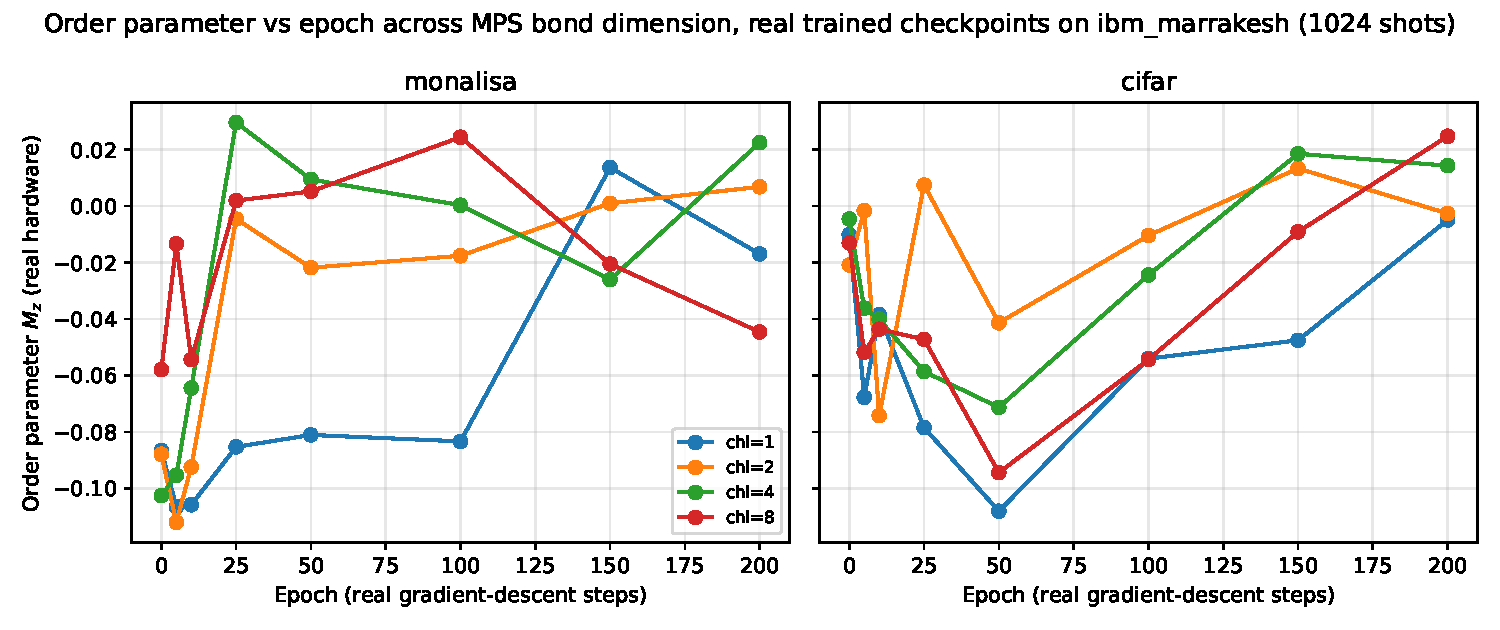
\includegraphics[width=0.9\linewidth]{figures/checkpoint_hardware_bond_dimension_order_parameter.pdf}
\caption{Bond-dimension checkpoint replay at 1024 shots on real IBM Quantum hardware. The plotted $M_z(t)$ traces use one representative patch and seed per image and $\chi$.}
\label{fig:supp_checkpoint_hardware_bond_dimension}
\end{figure}

\begin{table}[H]
\centering
\caption{Bond-dimension order-parameter replay jobs. Each job contains 64 circuits.}
\scriptsize
\resizebox{\linewidth}{!}{%
\begin{tabular}{llll}
\toprule
Platform & Backend & Shots & Job ID \\
\midrule
IBM hardware & \texttt{ibm\_marrakesh} & 256 & \texttt{d9hqu0jsbqfc73eqgr80} \\
IBM hardware & \texttt{ibm\_marrakesh} & 512 & \texttt{d9hr3d8gk0ls73f3elsg} \\
IBM hardware & \texttt{ibm\_marrakesh} & 1024 & \texttt{d9hr43l0k0jc738il8ug} \\
IonQ ideal simulator & \texttt{ionq\_simulator} & 256 & \texttt{019f9571-21d0-7339-9111-d31a308440a1} \\
IonQ ideal simulator & \texttt{ionq\_simulator} & 512 & \texttt{019f9573-1ed9-768c-9768-465fe75a409b} \\
IonQ ideal simulator & \texttt{ionq\_simulator} & 1024 & \texttt{019f9574-a981-71dd-94b0-9d8fb8968f49} \\
\bottomrule
\end{tabular}
}
\end{table}

\begin{figure}[H]
\centering
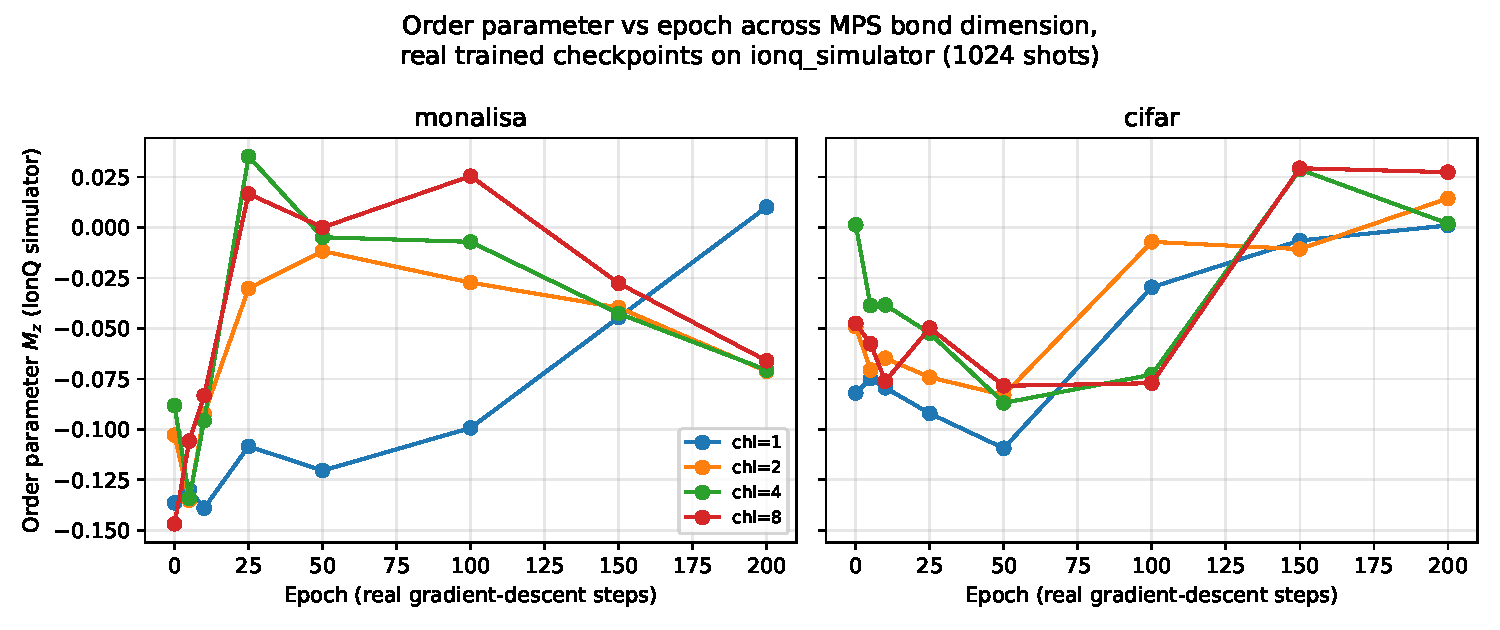
\includegraphics[width=0.9\linewidth]{figures/checkpoint_ionq_bond_dimension_order_parameter.pdf}
\caption{The same bond-dimension checkpoint replay as Figure~\ref{fig:supp_checkpoint_hardware_bond_dimension}, executed instead on the IonQ ideal cloud simulator at 1024 shots.}
\label{fig:supp_checkpoint_ionq_bond_dimension}
\end{figure}

Figure~\ref{fig:supp_checkpoint_ionq_bond_dimension} shows the corresponding IonQ traces: $\chi=1$ remains the most distinct trajectory on both images, the same qualitative pattern as Figure~\ref{fig:supp_checkpoint_hardware_bond_dimension}'s hardware replay, consistent with these being ideal-simulator and real-device executions of the identical checkpoint circuits rather than independent training runs.

We additionally replayed the three-basis energy-to-entanglement estimator for the same checkpoint grid. Each platform/shot job contains $2\times4\times8\times3=192$ circuits. At $\chi=1$, the MPS is a product state and the archived entropy sum is fixed at the numerical floor, $S=5.0\times10^{-6}$, compared with $S=0.014$--$0.045$ for $\chi\geq2$. Consequently, $R_{ES}=H/S$ reaches $O(10^5$--$10^6)$ through division by a near-zero denominator. We retain those rows in the machine-readable archive but exclude them from Figure~\ref{fig:supp_checkpoint_hardware_bond_dimension_res}; this is a construction-limit audit, not a physical divergence.

\begin{figure}[H]
\centering
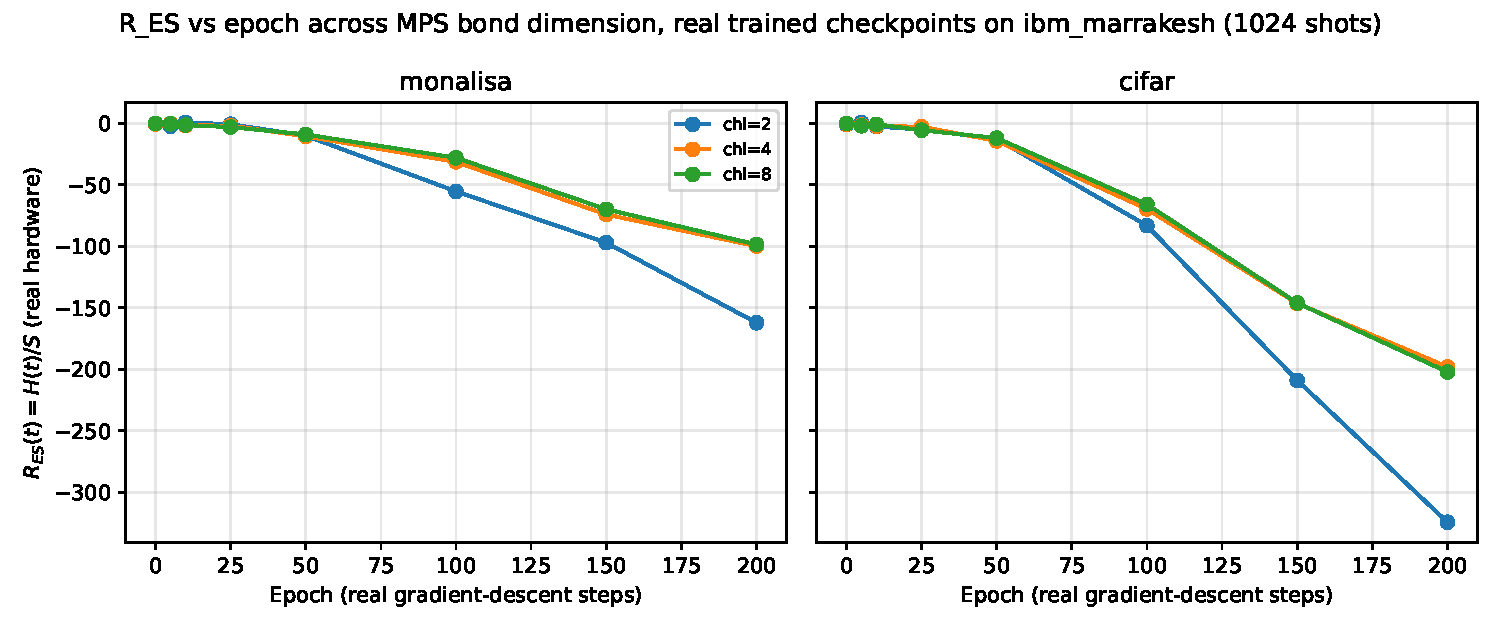
\includegraphics[width=0.9\linewidth]{figures/checkpoint_hardware_bond_dimension_r_es.pdf}
\caption{Energy-to-entanglement ratio across $\chi\in\{2,4,8\}$ at 1024 shots on real IBM Quantum hardware; $\chi=1$ is excluded because its product-state entropy is at the numerical floor.}
\label{fig:supp_checkpoint_hardware_bond_dimension_res}
\end{figure}

\begin{table}[H]
\centering
\caption{Bond-dimension $R_{ES}$ replay jobs. Each job contains 192 circuits over three measurement bases.}
\scriptsize
\resizebox{\linewidth}{!}{%
\begin{tabular}{llll}
\toprule
Platform & Backend & Shots & Job ID \\
\midrule
IBM hardware & \texttt{ibm\_marrakesh} & 256 & \texttt{d9hr44shonhs73adgq40} \\
IBM hardware & \texttt{ibm\_marrakesh} & 512 & \texttt{d9hr5u50k0jc738ilbs0} \\
IBM hardware & \texttt{ibm\_marrakesh} & 1024 & \texttt{d9hrb8shonhs73adh8mg} \\
IonQ ideal simulator & \texttt{ionq\_simulator} & 256 & \texttt{019f957f-dfbe-70fc-b6aa-b2398317f049} \\
IonQ ideal simulator & \texttt{ionq\_simulator} & 512 & \texttt{019f9584-4ba3-7224-ab7b-e81e32e6c1e2} \\
IonQ ideal simulator & \texttt{ionq\_simulator} & 1024 & \texttt{019f9586-4eb6-7596-ba47-dc6132c7f943} \\
\bottomrule
\end{tabular}
}
\end{table}

\begin{figure}[H]
\centering
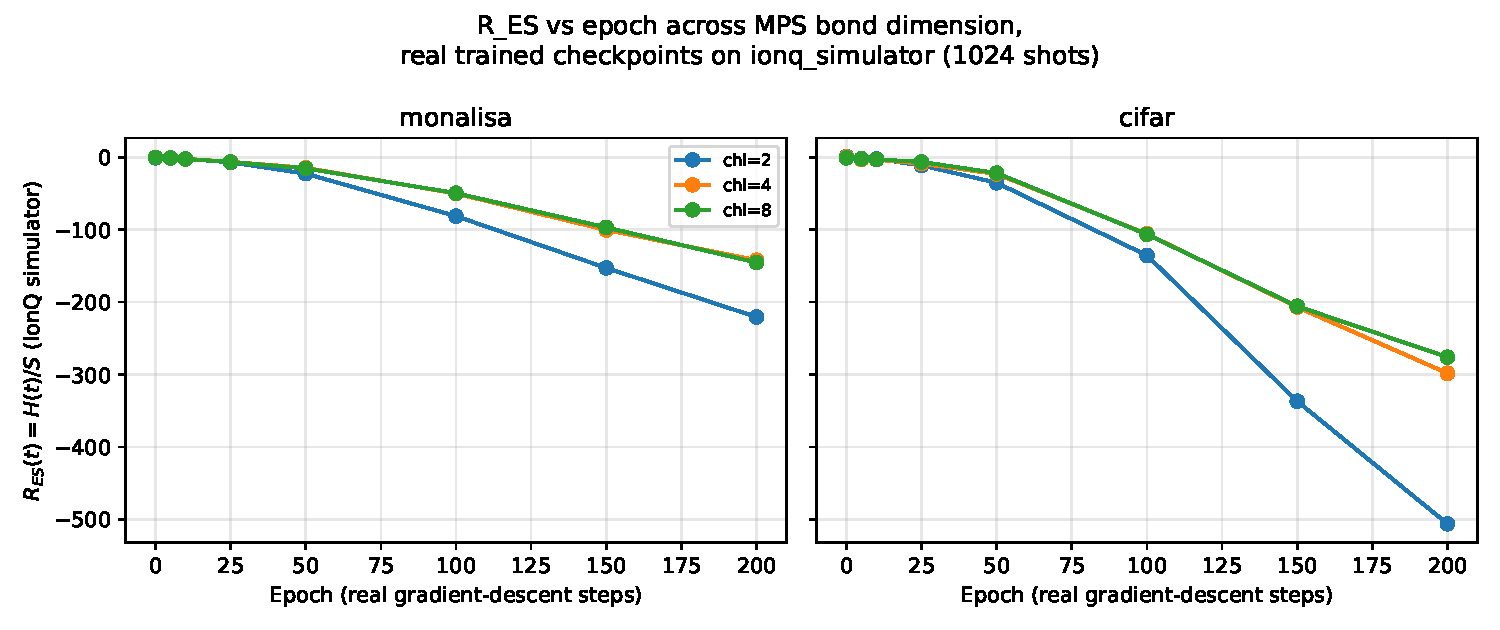
\includegraphics[width=0.9\linewidth]{figures/checkpoint_ionq_bond_dimension_r_es.pdf}
\caption{Energy-to-entanglement ratio across $\chi\in\{2,4,8\}$ at 1024 shots on the IonQ ideal cloud simulator, the same checkpoints and circuits as Figure~\ref{fig:supp_checkpoint_hardware_bond_dimension_res}; $\chi=1$ is excluded for the same numerical-floor reason.}
\label{fig:supp_checkpoint_ionq_bond_dimension_res}
\end{figure}

For $\chi\in\{2,4,8\}$, the $\chi=4$ and $\chi=8$ traces are close on both images, while $\chi=2$ becomes more negative by epoch 200, on both real hardware (Figure~\ref{fig:supp_checkpoint_hardware_bond_dimension_res}) and the IonQ ideal simulator (Figure~\ref{fig:supp_checkpoint_ionq_bond_dimension_res}). This single-patch, single-seed pattern is descriptive. It neither establishes a bond-dimension scaling law nor independently confirms the two-seed simulator observation about initialization sensitivity. The complete per-shot IBM and IonQ summaries are stored under \path{IBM_Cloud/outputs/checkpoint_bond_dimension_hardware_sweep/} and \path{IBM_Cloud/outputs/checkpoint_bond_dimension_temperature_hardware_sweep/}.

\subsection{Reconstruction Decode}
Hardware counts were converted to observable expectation values by the standard parity estimator, $\langle Z_i\rangle = \frac{1}{S}\sum_{\text{shots}} (-1)^{b_i}$ (identically for $X$, $Y$ after basis rotation), with pairwise correlators computed as the shot-weighted mean of $(-1)^{b_i+b_j}$ within the same measurement basis. The resulting observable vector, concatenated with the training-time positional encoding, was passed through the \emph{unmodified} trained decoder. No hardware-specific fine-tuning, error mitigation, or post-hoc calibration was applied.

\section{Reproducibility and Artifact Map}\leavevmode\par
The repository-level experiment drivers set Python, NumPy, and PyTorch random seeds explicitly. Unless a section states otherwise, multi-seed studies use seeds $\{0,1,2,3,4\}$; the reduced real-circuit topology confirmation and six-dataset reconstruction extension use $\{0,1,2\}$. Held-out samples are disjoint from their corresponding fitting samples, and each reported paired test preserves the pairing unit stated in its table or surrounding text (image within split, or seed after within-seed image aggregation). ``Mean $\pm$ std'' denotes the arithmetic mean and population-standard-deviation summary (NumPy \texttt{ddof=0}) over the unit named in the caption. Bootstrap intervals are percentile 95\% intervals; Wilcoxon values are two-sided signed-rank tests. No multiple-comparison correction is applied, so $p$-values should be interpreted as individual-comparison summaries rather than as a family-wise discovery analysis.

The current verification environment uses Python 3.11.9, PyTorch 2.6.0 with CUDA 12.4, PennyLane 0.42.3, Qiskit 2.5.0, NumPy 2.4.6, pandas 3.0.3, scikit-learn 1.9.0, quimb 1.11.2, cotengra 0.7.5, and autoray 0.6.12 on an NVIDIA GeForce GTX 1050. The package constraints are declared in \path{pyproject.toml}; because that file does not pin every dependency to an exact version, the versions above identify the environment used for this verification pass rather than claiming bitwise reproducibility across arbitrary future installations.

\begin{sloppypar}
The principal artifact map is as follows. The lowercase driver \path{main2/newHVK/run_newhvk_suite.py} generates the synthetic restricted-pair diagnostic under \path{main2/newHVK/results/full_ablation_suite/} and the held-out CIFAR-10 controls under \path{main2/newHVK/results/q1_validation/}; the six-dataset extension is generated by \path{main2/newHVK/run_multi_dataset_validation.py} and stored under \path{main2/newHVK/results/multi_dataset_validation/}. The newer experiment drivers use the repository's historically uppercase path: \path{Main2/newHVK/run_topology_comparison.py}, \path{Main2/newHVK/run_d4_symmetry_experiment.py}, and \path{Main2/newHVK/run_phase_transition_multi_dataset.py}, with outputs respectively under \path{Main2/newHVK/results/topology_comparison/}, \path{Main2/newHVK/results/d4_symmetry_experiment/}, and \path{Main2/newHVK/results/phase_transition_multi_dataset/}. The topology directory includes raw per-run JSON, summaries, paired statistics, and a surrogate manifest. Excluded legacy training-mode traces and any future deterministic evaluation-mode traces have distinct filenames and provenance fields. Path case is intentional and must be preserved on case-sensitive systems. Hardware-pilot result metadata and measured observable arrays are stored under \path{IBM_Cloud/outputs/hardware_reconstruction/} and \path{IBM_Cloud/outputs/hvk2d_cifar_hardware_reconstruction/}; bond-dimension hardware replays use the two output directories listed in Section~\ref{sec:supp_bond_dimension_hardware}. Raw and summary artifacts are retained separately so that manuscript means and uncertainty intervals can be recomputed without reading values from figures.
\end{sloppypar}

\section{Discussion}

\subsection{Task-Dependent Representational Scope}
The tie-with-classical outcome in Section~\ref{sec:holdout_headline} is consistent with a broader pattern in quantum machine learning: whether a quantum feature map or kernel offers an advantage over a classical model depends on the data, target, and comparison class rather than on the model label alone. At the resolution and patch size tested here, the empirical result is that local and raw-linear maps already capture the reconstruction signal available to the shared readout; we do not infer an entanglement property of the image distribution from that observation. The restricted diagnostic of Section~\ref{sec:restricted_ablation} is the contrasting case: its target is constructed around a distant-element product that the tested raw or local features cannot represent under the fixed linear readout, and the entangling channel separates in that setting. Together, the results delimit the tested operating regime: entangling observables are necessary within the restricted feature/readout class, but are not isolated as necessary for ordinary held-out reconstruction under the evaluated protocol.

\subsection{Design and Evaluation Guidelines}
We distill this ablation study into concrete guidance for evaluating hybrid quantum--classical vision models: (1) \emph{resource-match} every classical control to the quantum model's feature width and readout parameter count; (2) \emph{freeze-isolate} each trainable component independently before crediting any one of them with an observed gain; (3) \emph{audit every favorable diagnostic for target--feature leakage} by tracing target- and feature-construction code for shared subexpressions; (4) \emph{report held-out, not same-set, performance} as the primary evidence for a representation-learning claim; (5) \emph{report multiple seeds with error bars} on any comparison intended to support a quantitative claim.

\section{Conclusion}
The resource-matched, multi-seed study delineates the tested operating regime of HVK. Under a shared fitted readout, simple local/raw maps match or exceed the HVK2D pair-observable map on ordinary held-out reconstruction. The entangling observable channel separates on the restricted target constructed to require nonlocal correlations; separately, $D_4$ pooling enforces equivariance to numerical precision but does not improve held-out reconstruction accuracy in the tested experiment. On held-out CIFAR-10, local-observable and raw-linear controls reach $18.80\pm1.42$~dB compared with HVK2D's $18.12\pm1.54$~dB; seed-level inference gives a $-0.68$~dB HVK2D-minus-control difference (bootstrap 95\% CI $[-0.91,-0.46]$~dB; Wilcoxon $p=0.0625$, $n=5$). The same numerical direction appears on five further real datasets. These results motivate task-aligned HVK variants and strengthen the framework's evidentiary scope. The leakage and provenance audits contribute a transferable validation protocol, and Section~\ref{sec:hardware_methodology} provides the complete hardware-pilot methodology.

\part{References}
\addcontentsline{toc}{part}{References}
\begin{thebibliography}{99}
\bibitem{Araz2022} J. Y. Araz and M. Spannowsky, ``Classical versus quantum: Comparing tensor-network-based quantum circuits on Large Hadron Collider data,'' \textit{Physical Review A}, vol. 106, no. 6, p. 062423, 2022.
\bibitem{Bauer2020} B. Bauer, S. Bravyi, M. Motta, and G. K.-L. Chan, ``Quantum Algorithms for Quantum Chemistry and Quantum Materials Science,'' \textit{Chemical Reviews}, vol. 120, no. 22, pp. 12685--12717, 2020.
\bibitem{Bharti2022} K. Bharti, A. Cervera-Lierta, T. H. Kyaw, et al., ``Noisy intermediate-scale quantum (NISQ) algorithms,'' \textit{Reviews of Modern Physics}, vol. 94, p. 015004, 2022. arXiv:2101.08448.
\bibitem{Bronstein2021} M. M. Bronstein, J. Bruna, T. Cohen, and P. Veli\v{c}kovi\'c, ``Geometric Deep Learning: Grids, Groups, Graphs, Geodesics, and Gauges,'' 2021. arXiv:2104.13478.
\bibitem{Cerezo2021} M. Cerezo et al., ``Variational quantum algorithms,'' \textit{Nature Reviews Physics}, vol. 3, no. 9, pp. 625--644, 2021. arXiv:2012.09265.
\bibitem{Chakraborty2018} S. Chakraborty, S. B. Mandal, and S. H. Shaikh, ``Quantum image processing: challenges and future research issues,'' \textit{International Journal of Information Technology}, vol. 14, no. 1, pp. 475--489, 2022.
\bibitem{Chinni2023} L. K. Castelano, I. Cunha, F. S. Luiz, M. V. de Souza Prado, and F. F. Fanchini, ``Physics Informed Neural Networks Learning a Two-Qubit Hamiltonian,'' 2023. arXiv:2310.15148.
\bibitem{Cirac2021} J. I. Cirac, D. P\'erez-Garc\'ia, N. Schuch, and F. Verstraete, ``Matrix product states and projected entangled pair states: Concepts, symmetries, theorems,'' \textit{Reviews of Modern Physics}, vol. 93, no. 4, p. 045003, 2021.
\bibitem{Cohen2016} T. Cohen and M. Welling, ``Group Equivariant Convolutional Networks,'' in \textit{Proceedings of the 33rd International Conference on Machine Learning}, PMLR, vol. 48, 2016, pp. 2990--2999. arXiv:1602.07576.
\bibitem{Cong2019} I. Cong, S. Choi, and M. D. Lukin, ``Quantum Convolutional Neural Networks,'' \textit{Nature Physics}, vol. 15, pp. 1273--1278, 2019. arXiv:1810.03787.
\bibitem{Cotler2021} J. Cotler, H.-Y. Huang, and J. R. McClean, ``Revisiting dequantization and quantum advantage in learning tasks,'' 2021. arXiv:2112.00811.
\bibitem{Craps2024} B. Craps, M. De Clerck, O. Evnin, and P. Hacker, ``Integrability and complexity in quantum spin chains,'' \textit{SciPost Physics}, vol. 16, no. 2, p. 041, 2024.
\bibitem{Cunningham2024} J. Cunningham and J. Zhuang, ``Investigating and Mitigating Barren Plateaus in Variational Quantum Circuits: A Survey,'' \textit{Quantum Information Processing}, vol. 24, art. 48, 2025. arXiv:2407.17706.
\bibitem{Deshpande2024} A. Deshpande, M. Hinsche, K. Najafi, K. Sharma, R. Sweke, and C. Zoufal, ``Dynamic parameterized quantum circuits: expressive and barren-plateau free,'' 2024 (rev.\ 2025). arXiv:2411.05760.
\bibitem{Fei2021} S. M. Fei, ``Compressed Sensing Based on Tensor Network Machine Learning,'' \textit{Physical Science \& Biophysics Journal}, vol. 5, no. 1, Art. no. 000174, 2021, doi: 10.23880/psbj-16000174.
\bibitem{Franchini2017} F. Franchini, \textit{An Introduction to Integrable Techniques for One-Dimensional Quantum Systems}, Lecture Notes in Physics, vol. 940. Springer, 2017. arXiv:1609.02100.
\bibitem{Guala2023} D. Guala, S. Zhang, E. Cruz, C. A. Riofr\'io, J. Klepsch, and J. M. Arrazola, ``A Practical Overview of Image Classification with Variational Tensor-Network Quantum Circuits,'' \textit{Scientific Reports}, vol. 13, no. 1, p. 4427, 2023. arXiv:2209.11058.
\bibitem{Gyurik2023} C. Gyurik and V. Dunjko, ``Exponential separations between classical and quantum learners,'' 2023. arXiv:2306.16028.
\bibitem{Haga2024} A. Haga, ``Quantum annealing-based computed tomography using variational approach for a real-number image reconstruction,'' \textit{Physics in Medicine and Biology}, vol. 69, no. 4, Art. no. 04NT02, 2024, doi: 10.1088/1361-6560/ad2155.
\bibitem{Han2018} Z.-Y. Han, J. Wang, H. Fan, L. Wang, and P. Zhang, ``Unsupervised Generative Modeling Using Matrix Product States,'' \textit{Physical Review X}, vol. 8, no. 3, p. 031012, 2018. arXiv:1709.01662.
\bibitem{Havlicek2019} V. Havl{\'i}{\v c}ek, A. D. C{\'o}rcoles, K. Temme, A. W. Harrow, A. Kandala, J. M. Chow, and J. M. Gambetta, ``Supervised learning with quantum-enhanced feature spaces,'' \textit{Nature}, vol. 567, no. 7747, pp. 209--212, 2019. arXiv:1804.11326.
\bibitem{Huang2020Shadows} H.-Y. Huang, R. Kueng, and J. Preskill, ``Predicting many properties of a quantum system from very few measurements,'' \textit{Nature Physics}, vol. 16, pp. 1050--1057, 2020.
\bibitem{Huang2021PowerData} H.-Y. Huang, M. Broughton, M. Mohseni, R. Babbush, S. Boixo, H. Neven, and J. R. McClean, ``Power of data in quantum machine learning,'' \textit{Nature Communications}, vol. 12, no. 1, p. 2631, 2021. arXiv:2011.01938.
\bibitem{HuangExpGAN2020} H.-L. Huang et al., ``Experimental Quantum Generative Adversarial Networks for Image Generation,'' \textit{Physical Review Applied}, vol. 16, p. 024051, 2021. arXiv:2010.06201.
\bibitem{Hur2022} T. Hur, L. Kim, and D. K. Park, ``Quantum convolutional neural network for classical data classification,'' \textit{Quantum Machine Intelligence}, vol. 4, art. 3, 2022. arXiv:2108.00661.
\bibitem{HybridGANHighRes2022} S. L. Tsang, M. T. West, S. M. Erfani, and M. Usman, ``Hybrid Quantum-Classical Generative Adversarial Network for High Resolution Image Generation,'' \textit{IEEE Transactions on Quantum Engineering}, 2023. arXiv:2212.11614.
\bibitem{HybridLatentDiffusion2025} K. Yeter-Aydeniz, N. M. Bauer, P. Jain, and M. Masnick, ``Hybrid Quantum-Classical Latent Diffusion Models for Medical Image Generation,'' 2025. arXiv:2508.09903.
\bibitem{IonQBackends} IonQ, ``Backends,'' \textit{IonQ Quantum Cloud Documentation}. [Online]. Available: \url{https://docs.ionq.com/user-manual/backends}. Accessed: Jul. 24, 2026.
\bibitem{Jobst2024} B. Jobst, K. Shen, C. A. Riofr\'io, E. Shishenina, and F. Pollmann, ``Efficient MPS representations and quantum circuits from the Fourier modes of classical image data,'' \textit{Quantum}, vol. 8, p. 1544, 2024. arXiv:2311.07666.
\bibitem{Krizhevsky2009} A. Krizhevsky, ``Learning multiple layers of features from tiny images,'' University of Toronto, Technical Report, 2009.
\bibitem{Larocca2025} M. Larocca, S. Thanasilp, S. Wang, K. Sharma, J. Biamonte, P. J. Coles, L. Cincio, J. R. McClean, Z. Holmes, and M. Cerezo, ``Barren plateaus in variational quantum computing,'' \textit{Nature Reviews Physics}, vol. 7, pp. 174--189, 2025. arXiv:2405.00781.
\bibitem{Latorre2005} J. I. Latorre, ``Image compression and entanglement,'' 2005. arXiv:quant-ph/0510031.
\bibitem{Le2011} P. Q. Le, F. Dong, and K. Hirota, ``A flexible representation of quantum images for polynomial preparation, image compression, and processing operations,'' \textit{Quantum Information Processing}, vol. 10, pp. 63--84, 2011.
\bibitem{LeCun1998} Y. LeCun, L. Bottou, Y. Bengio, and P. Haffner, ``Gradient-based learning applied to document recognition,'' \textit{Proceedings of the IEEE}, vol. 86, no. 11, pp. 2278--2324, 1998, doi: 10.1109/5.726791.
\bibitem{Liu2021} Y. Liu, W.-J. Li, X. Zhang, M. Lewenstein, G. Su, and S.-J. Ran, ``Entanglement-Based Feature Extraction by Tensor Network Machine Learning,'' \textit{Frontiers in Applied Mathematics and Statistics}, 2021.
\bibitem{Liu2022} Z. Liu, P.-X. Shen, W. Li, L.-M. Duan, and D.-L. Deng, ``Quantum capsule networks,'' \textit{Quantum Science and Technology}, vol. 8, no. 1, p. 015016, 2022.
\bibitem{Mari2020} A. Mari, T. R. Bromley, J. Izaac, M. Schuld, and N. Killoran, ``Transfer learning in hybrid classical-quantum neural networks,'' \textit{Quantum}, vol. 4, p. 340, 2020. arXiv:1912.08278.
\bibitem{McClean2018} J. R. McClean, S. Boixo, V. N. Smelyanskiy, R. Babbush, and H. Neven, ``Barren plateaus in quantum neural network training landscapes,'' \textit{Nature Communications}, vol. 9, no. 1, p. 4812, 2018. arXiv:1803.11173.
\bibitem{Meyer2023} J. J. Meyer, M. Mularski, E. Gil-Fuster, A. A. Mele, F. Arzani, A. Wilms, and J. Eisert, ``Exploiting Symmetry in Variational Quantum Machine Learning,'' \textit{PRX Quantum}, vol. 4, p. 010328, 2023. arXiv:2205.06217.
\bibitem{MosaiQ2023} D. Silver, T. Patel, W. Cutler, A. Ranjan, H. Gandhi, and D. Tiwari, ``MosaiQ: Quantum Generative Adversarial Networks for Image Generation on NISQ Computers,'' in \textit{Proc. IEEE/CVF International Conference on Computer Vision (ICCV)}, 2023. arXiv:2308.11096.
\bibitem{Nau2023} M. A. Nau, A. H. Vija, W. Gohn, M. P. Reymann, and A. Maier, ``Exploring the Limitations of Hybrid Adiabatic Quantum Computing for Emission Tomography Reconstruction,'' \textit{Journal of Imaging}, vol. 9, no. 10, p. 221, 2023.
\bibitem{Nguyen2024EQNN} Q. T. Nguyen, L. Schatzki, P. Braccia, M. Ragone, P. J. Coles, F. Sauvage, M. Larocca, and M. Cerezo, ``Theory for Equivariant Quantum Neural Networks,'' \textit{PRX Quantum}, vol. 5, p. 020328, 2024. arXiv:2210.08566.
\bibitem{Park2024} C.-Y. Park and N. Killoran, ``Hamiltonian variational ansatz without barren plateaus,'' \textit{Quantum}, vol. 8, p. 1239, 2024. arXiv:2302.08529.
\bibitem{Peruzzo2014} A. Peruzzo, J. McClean, P. Shadbolt, et al., ``A variational eigenvalue solver on a quantum processor,'' \textit{Nature Communications}, vol. 5, p. 4213, 2014. arXiv:1304.3061.
\bibitem{Pesah2021} A. Pesah, M. Cerezo, S. Wang, T. Volkoff, A. T. Sornborger, and P. J. Coles, ``Absence of Barren Plateaus in Quantum Convolutional Neural Networks,'' \textit{Physical Review X}, vol. 11, p. 041011, 2021. arXiv:2011.02966.
\bibitem{Preskill2018} J. Preskill, ``Quantum Computing in the NISQ era and beyond,'' \textit{Quantum}, vol. 2, p. 79, 2018. arXiv:1801.00862.
\bibitem{QAEClassification2025} H. Asaoka and K. Kudo, ``Quantum autoencoders for image classification,'' \textit{Quantum Machine Intelligence}, vol. 7, p. 71, 2025. arXiv:2502.15254.
\bibitem{QCAE2023} J. Wu, H. Fu, M. Zhu, H. Zhang, W. Xie, and X.-Y. Li, ``Quantum circuit autoencoder,'' \textit{Physical Review A}, vol. 109, p. 032623, 2024. arXiv:2307.08446.
\bibitem{QIPSystematicReview2025} U. Farooq, P. Singh, and A. Kumar, ``A systematic review of quantum image processing: Representation, applications and future perspectives,'' \textit{Computer Science Review}, vol. 57, p. 100763, 2025.
\bibitem{QuantumDiffusion2024} M. K\"olle, G. Stenzel, J. Stein, S. Zielinski, B. Ommer, and C. Linnhoff-Popien, ``Quantum Denoising Diffusion Models,'' 2024. arXiv:2401.07049.
\bibitem{QuantumImageRepClassification2025} M. Parigi, M. Khosrojerdi, F. Caruso, and L. Banchi, ``Analysis of quantum image representations for supervised classification,'' \textit{AVS Quantum Science}, vol. 8, no. 1, p. 013801, 2026. arXiv:2507.22039.
\bibitem{QuantumKernelDefect2022} D. Beaulieu, D. Miracle, A. Pham, and W. Scherr, ``Quantum Kernel for Image Classification of Real World Manufacturing Defects,'' 2022. arXiv:2212.08693.
\bibitem{Romero2017} J. Romero, J. P. Olson, and A. Aspuru-Guzik, ``Quantum autoencoders for efficient compression of quantum data,'' \textit{Quantum Science and Technology}, vol. 2, p. 045001, 2017. arXiv:1612.02806.
\bibitem{Sauvage2024} F. Sauvage, M. Larocca, P. J. Coles, and M. Cerezo, ``Building Spatial Symmetries into Parameterized Quantum Circuits for Faster Training,'' \textit{Quantum Science and Technology}, vol. 9, p. 015029, 2024. arXiv:2207.14413.
\bibitem{Schatzki2024} L. Schatzki, M. Larocca, Q. T. Nguyen, F. Sauvage, and M. Cerezo, ``Theoretical Guarantees for Permutation-Equivariant Quantum Neural Networks,'' \textit{npj Quantum Information}, vol. 10, p. 12, 2024. arXiv:2210.09974.
\bibitem{Shi2022} J. Shi, W. Wang, X. Lou, S. Zhang, and X. Li, ``Parameterized Hamiltonian Learning With Quantum Circuit,'' \textit{IEEE Transactions on Pattern Analysis and Machine Intelligence}, vol. 45, no. 5, pp. 6086--6095, 2023.
\bibitem{Skolik2023} A. Skolik, M. Cattelan, S. Yarkoni, T. B\"ack, and V. Dunjko, ``Equivariant Quantum Circuits for Learning on Weighted Graphs,'' \textit{npj Quantum Information}, vol. 9, p. 47, 2023. arXiv:2205.06109.
\bibitem{Slabbert2024} D. Slabbert and F. Petruccione, ``Hybrid Quantum-Classical Feature Extraction approach for Image Classification using Autoencoders and Quantum SVMs,'' 2024. arXiv:2410.18814.
\bibitem{Stoudenmire2016} E. M. Stoudenmire and D. J. Schwab, ``Supervised Learning with Quantum-Inspired Tensor Networks,'' in \textit{Advances in Neural Information Processing Systems}, vol. 29, 2016. arXiv:1605.05775.
\bibitem{Tang2019} E. Tang, ``A quantum-inspired classical algorithm for recommendation systems,'' in \textit{Proceedings of the 51st Annual ACM SIGACT Symposium on Theory of Computing (STOC)}, 2019. arXiv:1807.04271.
\bibitem{Tilly2022} J. Tilly et al., ``The Variational Quantum Eigensolver: A review of methods and best practices,'' \textit{Physics Reports}, vol. 986, pp. 1--128, 2022.
\bibitem{Wang2023TN} M. Wang, Y. Pan, Z. Xu, G. Li, X. Yang, D. Mandic, and A. Cichocki, ``Tensor Networks Meet Neural Networks: A Survey and Future Perspectives,'' 2023. arXiv:2302.09019.
\bibitem{Wang2024QML} Y. Wang and J. Liu, ``A comprehensive review of Quantum Machine Learning: from NISQ to Fault Tolerance,'' \textit{Reports on Progress in Physics}, vol. 87, p. 116402, 2024. arXiv:2401.11351.
\bibitem{WangQAECompression2024} H. Wang, J. Tan, Y. Huang, and W. Zheng, ``Quantum image compression with autoencoders based on parameterized quantum circuits,'' \textit{Quantum Information Processing}, vol. 23, p. 41, 2024.
\bibitem{Weiler2019} M. Weiler and G. Cesa, ``General E(2)-Equivariant Steerable CNNs,'' in \textit{Advances in Neural Information Processing Systems}, vol. 32, 2019. arXiv:1911.08251.
\bibitem{West2023} M. West, M. Sevior, and M. Usman, ``Reflection Equivariant Quantum Neural Networks for Enhanced Image Classification,'' \textit{Machine Learning: Science and Technology}, vol. 4, p. 035027, 2023. arXiv:2212.00264.
\bibitem{West2024} M. West, J. Heredge, M. Sevior, and M. Usman, ``Provably Trainable Rotationally Equivariant Quantum Machine Learning,'' \textit{PRX Quantum}, vol. 5, p. 030320, 2024. arXiv:2311.05873. Erratum: \textit{PRX Quantum}, vol. 6, p. 020902, 2025; see also Z. Xiao and T. Li, ``Comment on `Provably Trainable Rotationally Equivariant Quantum Machine Learning','' arXiv:2504.16950, 2025.
\bibitem{West2025} P. San Sebastian, M. Ca\~{n}izo, and R. Or\'us, ``Image Classification with Rotation-Invariant Variational Quantum Circuits,'' \textit{Physical Review Research}, vol. 7, p. 013082, 2025. arXiv:2403.15031.
\bibitem{Wolberg1993} W. Wolberg, O. Mangasarian, N. Street, and W. Street, ``Breast Cancer Wisconsin (Diagnostic),'' UCI Machine Learning Repository, 1993, doi: 10.24432/C5DW2B.
\bibitem{Xiao2017} H. Xiao, K. Rasul, and R. Vollgraf, ``Fashion-MNIST: A novel image dataset for benchmarking machine learning algorithms,'' arXiv:1708.07747, 2017.
\bibitem{Xu2021} R. Xu, X. Wang, K. Chen, B. Zhou, and C. C. Loy, ``Positional Encoding as Spatial Inductive Bias in GANs,'' in \textit{Proceedings of the IEEE/CVF Conference on Computer Vision and Pattern Recognition (CVPR)}, 2021, pp. 13564--13573.
\bibitem{Yang2023} J. Yang et al., ``MedMNIST v2---A large-scale lightweight benchmark for 2D and 3D biomedical image classification,'' \textit{Scientific Data}, vol. 10, Art. no. 41, 2023, doi: 10.1038/s41597-022-01721-8.
\bibitem{Yao2017} X. Yao et al., ``Quantum Image Processing and Its Application to Edge Detection: Theory and Experiment,'' \textit{Physical Review X}, vol. 7, no. 3, p. 031041, 2017.
\bibitem{Zaman2023} K. Zaman, A. Marchisio, M. A. Hanif, and M. Shafique, ``A Survey on Quantum Machine Learning: Current Trends, Challenges, Opportunities, and the Road Ahead,'' 2023. arXiv:2310.10315.
\bibitem{Zhai2025} X. Zhai, T. Xiao, J. Huang, J. Fan, and G. Zeng, ``Quantum neural compressive sensing for ghost imaging,'' \textit{Physical Review Applied}, vol. 23, no. 1, p. 014018, 2025.
\bibitem{Zhang2013} Y. Zhang, K. Lu, Y. Gao, and M. Wang, ``NEQR: A novel enhanced quantum representation of digital images,'' \textit{Quantum Information Processing}, vol. 12, no. 8, pp. 2833--2860, 2013.
\bibitem{Zhou2017} R. Zhou, W. Hu, P. Fan, and H. Ian, ``Quantum realization of the bilinear interpolation method for NEQR,'' \textit{Scientific Reports}, vol. 7, no. 1, p. 2511, 2017.
\bibitem{Zoufal2019} C. Zoufal, A. Lucchi, and S. Woerner, ``Quantum Generative Adversarial Networks for Learning and Loading Random Distributions,'' \textit{npj Quantum Information}, vol. 5, p. 103, 2019. arXiv:1904.00043.
\end{thebibliography}

\end{document}
